% !TEX TS-program = pdflatex
% !TEX encoding = UTF-8 Unicode

\documentclass[a4paper,
    11pt,
    normalheadings,
%   parskip,
    parindent,
%   draft,
%   final,
%   bibgerm,
%   german,
    UKenglish,
%   twoside,
%   twocolum,
%   openright,  % Kap.beginn immer rechts! (fkt. nur bei report, nicht bei article)
    abstracton,
    ]{scrartcl}
\usepackage[english]{babel}
\usepackage[utf8]{inputenc} % set input encoding (not needed with XeLaTeX)

%%% Examples of Article customizations
% These packages are optional, depending whether you want the features they provide.
% See the LaTeX Companion or other references for full information.

%%% PAGE DIMENSIONS
\usepackage{geometry} % to change the page dimensions
\geometry{a4paper} % or letterpaper (US) or a5paper or....
% \geometry{margins=2in} % for example, change the margins to 2 inches all round
% \geometry{landscape} % set up the page for landscape
%   read geometry.pdf for detailed page layout information

\usepackage{graphicx} % support the \includegraphics command and options

\usepackage[parfill]{parskip} % Activate to begin paragraphs with an empty line rather than an indent

%%% PACKAGES
\usepackage{booktabs} % for much better looking tables
\usepackage{alltt} % provides alltt enviroment which allows \emph{}ed text
\usepackage{array} % for better arrays (eg matrices) in maths
\usepackage{paralist} % very flexible & customisable lists (eg. enumerate/itemize, etc.)
\usepackage{verbatim} % adds environment for commenting out blocks of text & for better verbatim
\usepackage{subfig} % make it possible to include more than one captioned figure/table in a single float
% These packages are all incorporated in the memoir class to one degree or another...


\usepackage[colorlinks,urlcolor=blue,plainpages=false]{hyperref}
\usepackage{embedfile}        % Provides \embedfile[filename=foo, desc={bar}]{file}
\usepackage{hyperxmp}         % To be have an XMP Data Stream f.e. to include the license

% \usepackage{newcent}  % Different Font, looks bigger

\usepackage{ifthen}

\usepackage[
    T1, % this is good for Umlauts
%   OT1 % This breaks Umlauts
       ]{fontenc}

%%% HEADERS & FOOTERS
\usepackage{fancyhdr} % This should be set AFTER setting up the page geometry
\pagestyle{fancy} % options: empty , plain , fancy
\renewcommand{\headrulewidth}{0pt} % customise the layout...
\lhead{}\chead{}\rhead{}
\lfoot{}\cfoot{\thepage}\rfoot{}

%%% SECTION TITLE APPEARANCE
\usepackage{sectsty}
\allsectionsfont{\sffamily\mdseries\upshape} % (See the fntguide.pdf for font help)
% (This matches ConTeXt defaults)

%%% ToC (table of contents) APPEARANCE
\usepackage[nottoc,notlof,notlot]{tocbibind} % Put the bibliography in the ToC
\usepackage[titles,subfigure]{tocloft} % Alter the style of the Table of Contents
\renewcommand{\cftsecfont}{\rmfamily\mdseries\upshape}
\renewcommand{\cftsecpagefont}{\rmfamily\mdseries\upshape} % No bold!

\usepackage{listings}

\usepackage{movie15}


%%% END Article customizations

%%% The "real" document content comes below...

% Title Page
\newcommand{\mytitle}{Lab07.5: Honeypot Network Analysis}
\subject{Report\\%
    Forensics\\%
    Summersemester 2010\\%
    CA643\\%
    Charlie Daly}
\title{\mytitle{}}
%\subtitle{}
\author{
    cand. Dipl. Inf. Tobias Müller <\href{mailto:muellet2@computing.dcu.ie?subject=ss10-forensic-lab08}{muellet2@}>, 59212333 \and
    BSc. Anthony Walters <\href{mailto:waltera3@computing.dcu.ie?subject=ss10-forensic-lab08}{waltera3@}>, 59213102 \and Conor Lynch <\href{mailto:conor.lynch36@mail.dcu.ie}{lynchc36@}>, 55619599}
% \institute[Mathe - UniHH]{Fachbereich Mathematik\\
%         Universit\"at Hamburg}
% \logo{\includegraphics[height=0.5cm]{cinsects-blue}}
% \titlegraphic{\includegraphics[width=1.5cm]{fsr-logo}}
\date{\today}


\hypersetup{
        pdftitle={\mytitle{}},
        pdfauthor={Tobias Mueller, Anthony Walters, Conor Lynch},
        pdfsubject={Forensics},
        pdfkeywords={uni, linux, windows, ca643, forensics, binary, data, vis},
        pdflang=en,
        pdfcopyright={This work is licensed to the public under the Creative Commons Attribution-Non-Commercial-Share Alike 3.0 Germany License.},
        pdflicenseurl={http://creativecommons.org/licenses/by-nc-sa/3.0/de/}
}

\hyphenation{Infor-mations-sys-teme}
\hyphenation{\"{o}ko-logischen}

\newcommand{\note}[1]{#1}
\renewcommand{\comment}[1]{}
\newcommand{\inlinequote}[1]{``\textit{#1}''}
\newcommand{\FIXME}[1]{\mbox{}\marginpar{\footnotesize\raggedright\hspace{0pt}\color{red}\emph{#1}}}

\begin{document}
\selectlanguage{english}
\maketitle


\section{Introduction} \label{sec:intro}
In this Lab report, we will examine recorded traffic and console in- and output of a honeypot that has been ``hacked''.
The network traffic was recorded into a file in the well known pcap (\emph{p}acket \emph{cap}ture) format\footnote{\url{http://www.tcpdump.org/pcap3_man.html}}.
Serial I/O was saved in a SQLite3 database along with a timestamp.

Using Wireshark on the pcap file, we can see, by selecting Statistics$\rightarrow$Summary, that the capture file identifies itself as being taken at 2009-01-14 16:24:07 and the capture lasts 11.5 days until 2009-01-26 10:05:01.
In total, 4323191 IP packets, which sum up to 673023355 bytes (more than 0.6GB),   were sent.


\begin{figure}
\begin{alltt}
===================================================================
Protocol Hierarchy Statistics
Filter: frame

frame                                    frames:4323191 bytes:673023355
  eth                                    frames:4323191 bytes:673023355
    ip                                   frames:4323191 bytes:673023355
      icmp                               frames:22450 bytes:3949050
      tcp                                frames:4114918 bytes:650584934
        ssh                              frames:53424 bytes:12207167
          malformed                      frames:337 bytes:33770
        http                             frames:40 bytes:8896
        tcp.segments                     frames:1428 bytes:231235
          ipdc                           frames:1344 bytes:214833
            malformed                    frames:1344 bytes:214833
              ipdc                       frames:3 bytes:462
                malformed                frames:3 bytes:462
          gryphon                        frames:12 bytes:1604
        irc                              frames:457287 bytes:51115233
        data                             frames:27230 bytes:3161813
      udp                                frames:185823 bytes:18489371
        dns                              frames:185432 bytes:18411089
          malformed                      frames:2 bytes:120
===================================================================
\end{alltt}
  \caption{Traffic by Protocol, generated with \texttt{tshark -q -r capture.cap -z io,phs}}
  \label{protocol-hierachy}
\end{figure}

A breakdown of the traffic by protocol can be found in
\hyperref[protocol-hierachy]{figure \ref*{protocol-hierachy}}
(which is stripped to weed out unnecessary information).
Interesting facts that can be read are:
\begin{itemize}
    \item Most of the data (51MB) was trasferred using Internet Relay Chat (\emph{IRC}), followed by 18MB via Domain Name Service (\emph{DNS}), followed by 12MB Secure Shell (\emph{SSH}).
    \item That matches the total number of packets: $\sim$500k for IRC and $\sim$180 DNS. SSH was used very efficiently: only $\sim$50k packets were sent.
\end{itemize}
Further analysis will thus focus on the reason for these  packets, i.e.\, whether they were used for an attack or to do actual communication.


To get an idea of the distribution of traffic over time, i.e. if an IRC server was attacked constantly or one time with a huge number of packets, a timeline of the traffic can be seen in
\hyperref[pic:traffic-packets-over-time]{figure \ref*{pic:traffic-packets-over-time}}.

We can see one big peak near the beginning of the capture indicating many packets being sent.
The following peaks are not nearly as big as the first one but still indicate a lot of packets.

\begin{figure}
  \begin{center}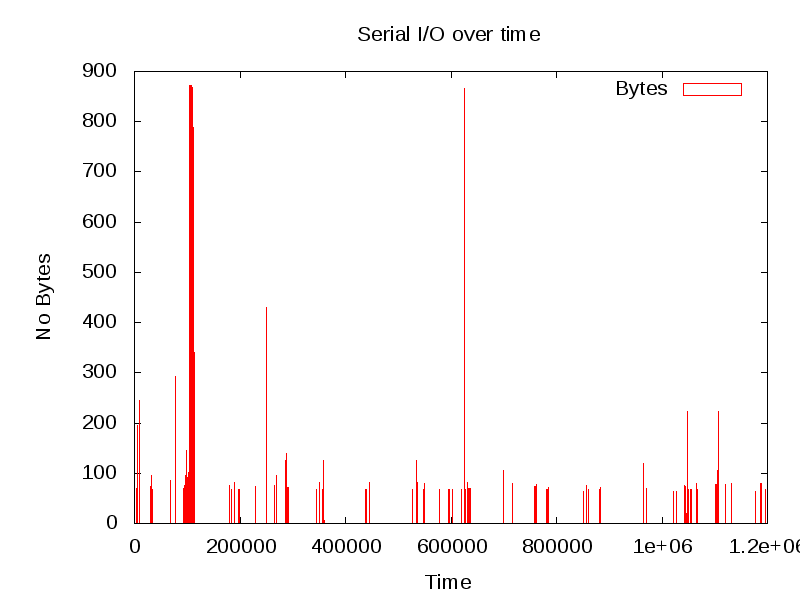
\includegraphics[width=0.8\textwidth]{bin/serial-io-over-time.png}\end{center}
  \caption{Serial in/output over time, we see when the attacker connected} %FIXME: Better interpretation
  \label{pic:serial-io-over-time}
\end{figure}
The captured in- and output of the serial console can be graphed over time as well.
We see in
\hyperref[pic:serial-io-over-time]{figure \ref*{pic:serial-io-over-time}}
that the attackers caused serial I/O regularly with a few noteworthy exceptions.
Two peaks, which happen to match the traffic I/O shown in
 \hyperref[pic:traffic-packets-over-time]{figure \ref*{pic:traffic-packets-over-time}}
indicate heavy usage, i.e.\, an attack.
It does not come as a big surprise that the figure for the serial I/O matches the  figure for the traffic I/O, because at least the serial in- or ouput needs to be transferred to the attacker which is connected to the honeypot via SSH.




% \section{Visualising Network Traffic}
To aid analysis of the given 700MB network dump, we tried to use visualisation techniques.
Unfortunately, good visualisation tools which are easy to use, scale well with our big amount of data and are free, do not exist.
Or if they do, they are very well hidden.
But if tools existed, they can be expected to become known and famous within a short time because they would be announced and praised on visualisation hotspots on the Internet\footnote{\url{http://vizsec.org/} or \url{http://secviz.org/}}.



\begin{figure}
    \begin{center}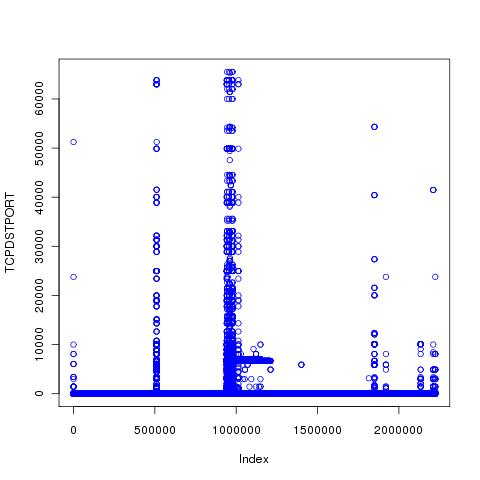
\includegraphics[width=\textwidth]{bin/lab07-tcpdstport_syn1_ack0.png}\end{center}
    \caption{Destination Ports over time}
    \label{pic:dest-ports-over-time} %FIXME: Make the background transparent.
\end{figure}
\hyperref[pic:dest-ports-over-time]{Figure \ref*{pic:dest-ports-over-time}}
shows the TCP destination ports over time.
We can see constant traffic on port 22, a few port scans over every port and a lot of IRC traffic to port 6667 in the middle of the observed traffic.
This is particularly interesting, because as IRC traffic, as in \autoref{sec:intro}, is one of the most present protocols in the capture.





In the rest of this report, we will first evaluate a set of tools that we used or tried to use in \autoref{sec:evaluating-tools}.
In \autoref{sec:http-traffic} we will identify and discuss packets that were related to HTTP traffic, including a set of tools that were later used to launch attacks on other networks.
\autoref{sec:ssh-traffic} then will investigate on the third most spoken protocol in the packet capture: SSH.
This will lead to \autoref{sec:slammer} which discusses an attack launched on other network using a vulnerability in MSSQL which was patched mid 2002 with MS02-039.
In \autoref{sec:davix} we will discuss our methods of analysing the network traffic and find new insights.
These will then be used in \autoref{sec:irc-traffic} to find information about the most dominantly used service in capture: IRC.
Finally, we will conclude our findings in \autoref{sec:conclusion}.



\section{Evaluating Tools} \label{sec:evaluating-tools}
A consiberable amount of time was spent on researching and evaluating tools that are capable of visualising a massive amount of data and networking data in particular.

We tried the following tools:
\begin{description}
    \item[\href{http://sourceforge.net/projects/safemap/}{Safe Mapping and Reporting Tool (SMART)}]
        is written in PERL and depends on many other PERL packages.
        Some of them are not packaged for Ubuntu which makes installation of these dependencies hard.
        Although there is the Comprehensive PERL Archive Network (CPAN) which is supposed to ease installation of dependencies, it is not really easy to use, because it firstly requires elevated privileges and secondly does not know about the needed modules.
        Although these problems are not unsolvable, we decided to not further try to get SMART up and running.

    \item[\href{http://www.grotto-group.com/~gulfie/projects/analysis/tcpdump2dot/gallery/}{tcpdump2dot}]
        looks solid but not as beautiful as the using tcpdump, afterglow and GraphViz so we did not consider it as an alternative.
        It's feature is, though, that it does the analysis and rendering automatically.
        There is no wrapper around afterglow and friends, that just renders a picture in an automated manner.


    \item[\href{http://www.parseerror.com/pizza/lanmap/}{lanmap}]
        Unfortunately, this project does not exist anymore.
        But its successor is called \emph{lanmap2} and will be described below.

    \item[\href{http://github.com/pizza/lanmap2}{lanmap2}]
        While this tools looks interesting, it expects the data to be present in a SQL database.
        It does not allow data to be obtained using the PCap file format.
        Again, we could have parsed the PCap file and entered every packet into the SQL database, but due to timecontraints we did not.

    \item[\href{http://www.doxpara.com}{Xovi}]
        Dan Kaminsky, who is a well known and respected member of the computer security community, has released a network visualisation tool during the 22nd annual Chaos Communication Conference (22C3) held by the German Chaos Computer Club (CCC)\footnote{cmp. \url{http://events.ccc.de/congress/2005/fahrplan/events/1108.de.html}}.
        Dan is also very well known for his attacks on DNS in summer 2008.
        Interestingly enough, his own DNS zone is configured to return a link local IP address\footnote{\url{http://tools.ietf.org/html/rfc5735}}, namely 169.254.0.0.
        This is very worrying given that Dan Kaminsky was hacked (pwned) himself\footnote{cmp. the eZine which is well worth a read: \url{http://seclists.org/fulldisclosure/2009/Jul/att-495/zf05.txt}} in summer 2009.
        But a personal communication reveals that the DNS setup is indeed a deliberatly chosen configuration and the intention is to bring correct DNS information back up soon.
        Anyway, the tool is not available at the moment.

    \item[\href{http://www.rumint.org/}{RUMINT}]
        is very interesting, because it is written in Visual Basic.
        \begin{figure}
            \begin{center}\includemovie[autoplay,label=csimovie,controls=true]{0.7\textwidth}{15em}{bin/CSI-Miami-VB-GUI.mp4}\end{center}
            \caption{Snippet of a CSI Miami episode using VisualBasic to trace an IP address}
        \end{figure}
        Although (or better: because) CSI Miami uses VisualBasic, as shown in \movieref{csimovie}{figure 4}, we immediately stopped considering it to be a useful tool.


    \item[\href{http://www.gephi.org}{Gephi}]
        ``is an open source software for graph and network analysis. It uses a 3D render engine to display large networks in real-time and to speed up the exploration. A flexible and multi-task architecture brings new possibilities to work with complex data sets and produce valuable visual results.''

        At least these are the claims made by the paper introducing Gephi\footnote{\url{http://www.aaai.org/ocs/index.php/ICWSM/09/paper/view/154}}.
        It is a Free Software tool made by an academic, written in Java and looks very promising.
        Sadly, we could not use it because it does not import data from anything else except a MySQL database.
        It also consumes a considerable amount of resources of our working machines.
        But more confunsingly: We were not able to create graphs!
        We do consider ourselves to be technically savvy, but the tool did not allow us to modify out created node or connect them with an edge.
        But even if it did, we would not have clicked the graph together manually anyway.
        So although Gephi looks very promising, we had to search for different tools.

    \item[\href{http://www.wallinfire.net/picviz/screenshots/index.html}{picviz}]
        looked promising, especially since it is a project with strong focus on networks and auditing.
        We tried to use it to visualise multidimensional data such as packets (time, source IP, destination IP, ...) but we had limited success.
        While the produced images are generally visually appealing and transferred the information in a smart way, we were not able to render a picture with a resolution good enough for a report.
    \begin{table}
        \begin{center}
            \begin{tabular}{r@{: }l}
            \hline
            CPU & Intel Core 2 Duo, 2x 2.6GHz\\
            RAM & 8GB\\
            Swap & 150GB\\\hline
        \end{tabular}
        \end{center}
        \caption{Data of the machine that tried to run picviz}
        \label{table:machinedata}
    \end{table}
        Higher quality images were tried to be rendered on the machine with the specs given in  \autoref{table:machinedata}, but even of that rather beefy computer, PicViz did not create an image but rather ran out of memory.
\end{description}



\begin{figure}
% % CSV file created with pcapaggregate.py jubrowska-capture_1.dump 600
% % rendered with gnuplot:
% %
% % set title "Packets over time"
% % set xlabel "Time"
% % set ylabel "No Packets"
% % set datafile separator ","
% % plot "/tmp/jubrowska-capture_1.dump.aggregate-600.csv" using ($1-1231950247):2 title "Packets" with linespoint
%% Hmpf. this is really annoying because Gobby does't let me fold it away.
% GNUPLOT: LaTeX picture
\setlength{\unitlength}{0.240900pt}
\ifx\plotpoint\undefined\newsavebox{\plotpoint}\fi
\sbox{\plotpoint}{\rule[-0.200pt]{0.400pt}{0.400pt}}%
\begin{picture}(1500,900)(0,0)
\sbox{\plotpoint}{\rule[-0.200pt]{0.400pt}{0.400pt}}%
\put(271.0,131.0){\rule[-0.200pt]{4.818pt}{0.400pt}}
\put(251,131){\makebox(0,0)[r]{ 0}}
\put(1430.0,131.0){\rule[-0.200pt]{4.818pt}{0.400pt}}
\put(271.0,239.0){\rule[-0.200pt]{4.818pt}{0.400pt}}
\put(251,239){\makebox(0,0)[r]{ 100000}}
\put(1430.0,239.0){\rule[-0.200pt]{4.818pt}{0.400pt}}
\put(271.0,346.0){\rule[-0.200pt]{4.818pt}{0.400pt}}
\put(251,346){\makebox(0,0)[r]{ 200000}}
\put(1430.0,346.0){\rule[-0.200pt]{4.818pt}{0.400pt}}
\put(271.0,454.0){\rule[-0.200pt]{4.818pt}{0.400pt}}
\put(251,454){\makebox(0,0)[r]{ 300000}}
\put(1430.0,454.0){\rule[-0.200pt]{4.818pt}{0.400pt}}
\put(271.0,562.0){\rule[-0.200pt]{4.818pt}{0.400pt}}
\put(251,562){\makebox(0,0)[r]{ 400000}}
\put(1430.0,562.0){\rule[-0.200pt]{4.818pt}{0.400pt}}
\put(271.0,669.0){\rule[-0.200pt]{4.818pt}{0.400pt}}
\put(251,669){\makebox(0,0)[r]{ 500000}}
\put(1430.0,669.0){\rule[-0.200pt]{4.818pt}{0.400pt}}
\put(271.0,777.0){\rule[-0.200pt]{4.818pt}{0.400pt}}
\put(251,777){\makebox(0,0)[r]{ 600000}}
\put(1430.0,777.0){\rule[-0.200pt]{4.818pt}{0.400pt}}
\put(271.0,131.0){\rule[-0.200pt]{0.400pt}{4.818pt}}
\put(271,90){\makebox(0,0){ 0}}
\put(271.0,757.0){\rule[-0.200pt]{0.400pt}{4.818pt}}
\put(468.0,131.0){\rule[-0.200pt]{0.400pt}{4.818pt}}
\put(468,90){\makebox(0,0){ 200000}}
\put(468.0,757.0){\rule[-0.200pt]{0.400pt}{4.818pt}}
\put(664.0,131.0){\rule[-0.200pt]{0.400pt}{4.818pt}}
\put(664,90){\makebox(0,0){ 400000}}
\put(664.0,757.0){\rule[-0.200pt]{0.400pt}{4.818pt}}
\put(861.0,131.0){\rule[-0.200pt]{0.400pt}{4.818pt}}
\put(861,90){\makebox(0,0){ 600000}}
\put(861.0,757.0){\rule[-0.200pt]{0.400pt}{4.818pt}}
\put(1057.0,131.0){\rule[-0.200pt]{0.400pt}{4.818pt}}
\put(1057,90){\makebox(0,0){ 800000}}
\put(1057.0,757.0){\rule[-0.200pt]{0.400pt}{4.818pt}}
\put(1254.0,131.0){\rule[-0.200pt]{0.400pt}{4.818pt}}
\put(1254,90){\makebox(0,0){ 1e+06}}
\put(1254.0,757.0){\rule[-0.200pt]{0.400pt}{4.818pt}}
\put(1450.0,131.0){\rule[-0.200pt]{0.400pt}{4.818pt}}
\put(1450,90){\makebox(0,0){ 1.2e+06}}
\put(1450.0,757.0){\rule[-0.200pt]{0.400pt}{4.818pt}}
\put(271.0,131.0){\rule[-0.200pt]{0.400pt}{155.621pt}}
\put(271.0,131.0){\rule[-0.200pt]{284.021pt}{0.400pt}}
\put(1450.0,131.0){\rule[-0.200pt]{0.400pt}{155.621pt}}
\put(271.0,777.0){\rule[-0.200pt]{284.021pt}{0.400pt}}
% \put(70,454){\makebox(0,0){No Packets}}
\put(860,29){\makebox(0,0){Time}}
\put(860,839){\makebox(0,0){Packets over time}}
\put(1290,737){\makebox(0,0)[r]{Packets}}
\put(1310.0,737.0){\rule[-0.200pt]{24.090pt}{0.400pt}}
\put(271,131){\usebox{\plotpoint}}
\put(274.67,131){\rule{0.400pt}{0.964pt}}
\multiput(274.17,131.00)(1.000,2.000){2}{\rule{0.400pt}{0.482pt}}
\put(275.67,131){\rule{0.400pt}{0.964pt}}
\multiput(275.17,133.00)(1.000,-2.000){2}{\rule{0.400pt}{0.482pt}}
\put(271.0,131.0){\rule[-0.200pt]{0.964pt}{0.400pt}}
\put(277,131){\usebox{\plotpoint}}
\put(295,130.67){\rule{0.241pt}{0.400pt}}
\multiput(295.00,130.17)(0.500,1.000){2}{\rule{0.120pt}{0.400pt}}
\put(296,130.67){\rule{0.241pt}{0.400pt}}
\multiput(296.00,131.17)(0.500,-1.000){2}{\rule{0.120pt}{0.400pt}}
\put(296.67,131){\rule{0.400pt}{1.204pt}}
\multiput(296.17,131.00)(1.000,2.500){2}{\rule{0.400pt}{0.602pt}}
\put(297.67,131){\rule{0.400pt}{1.204pt}}
\multiput(297.17,133.50)(1.000,-2.500){2}{\rule{0.400pt}{0.602pt}}
\put(277.0,131.0){\rule[-0.200pt]{4.336pt}{0.400pt}}
\put(299,131){\usebox{\plotpoint}}
\put(298.67,131){\rule{0.400pt}{137.795pt}}
\multiput(298.17,131.00)(1.000,286.000){2}{\rule{0.400pt}{68.897pt}}
\put(299.67,131){\rule{0.400pt}{137.795pt}}
\multiput(299.17,417.00)(1.000,-286.000){2}{\rule{0.400pt}{68.897pt}}
\put(301,131){\usebox{\plotpoint}}
\put(301.0,131.0){\rule[-0.200pt]{13.490pt}{0.400pt}}
\put(356.67,133){\rule{0.400pt}{0.723pt}}
\multiput(356.17,133.00)(1.000,1.500){2}{\rule{0.400pt}{0.361pt}}
\put(357.0,131.0){\rule[-0.200pt]{0.400pt}{0.482pt}}
\put(358.0,136.0){\rule[-0.200pt]{0.482pt}{0.400pt}}
\put(359.67,135){\rule{0.400pt}{0.964pt}}
\multiput(359.17,137.00)(1.000,-2.000){2}{\rule{0.400pt}{0.482pt}}
\put(360.67,132){\rule{0.400pt}{0.723pt}}
\multiput(360.17,133.50)(1.000,-1.500){2}{\rule{0.400pt}{0.361pt}}
\put(360.0,136.0){\rule[-0.200pt]{0.400pt}{0.723pt}}
\put(362.0,131.0){\usebox{\plotpoint}}
\put(362.0,131.0){\rule[-0.200pt]{0.482pt}{0.400pt}}
\put(363.67,132){\rule{0.400pt}{1.445pt}}
\multiput(363.17,132.00)(1.000,3.000){2}{\rule{0.400pt}{0.723pt}}
\put(364.67,138){\rule{0.400pt}{0.482pt}}
\multiput(364.17,138.00)(1.000,1.000){2}{\rule{0.400pt}{0.241pt}}
\put(364.0,131.0){\usebox{\plotpoint}}
\put(366,140){\usebox{\plotpoint}}
\put(365.67,138){\rule{0.400pt}{0.482pt}}
\multiput(365.17,139.00)(1.000,-1.000){2}{\rule{0.400pt}{0.241pt}}
\put(367.0,138.0){\usebox{\plotpoint}}
\put(367.0,139.0){\rule[-0.200pt]{0.482pt}{0.400pt}}
\put(369.0,138.0){\usebox{\plotpoint}}
\put(369.0,138.0){\usebox{\plotpoint}}
\put(370,137.67){\rule{0.241pt}{0.400pt}}
\multiput(370.00,138.17)(0.500,-1.000){2}{\rule{0.120pt}{0.400pt}}
\put(370.0,138.0){\usebox{\plotpoint}}
\put(371.0,138.0){\rule[-0.200pt]{1.445pt}{0.400pt}}
\put(377,137.67){\rule{0.241pt}{0.400pt}}
\multiput(377.00,138.17)(0.500,-1.000){2}{\rule{0.120pt}{0.400pt}}
\put(378,137.67){\rule{0.241pt}{0.400pt}}
\multiput(378.00,137.17)(0.500,1.000){2}{\rule{0.120pt}{0.400pt}}
\put(377.0,138.0){\usebox{\plotpoint}}
\put(379,139){\usebox{\plotpoint}}
\put(379,137.67){\rule{0.241pt}{0.400pt}}
\multiput(379.00,138.17)(0.500,-1.000){2}{\rule{0.120pt}{0.400pt}}
\put(380,138){\usebox{\plotpoint}}
\put(380.0,138.0){\rule[-0.200pt]{2.891pt}{0.400pt}}
\put(392,137.67){\rule{0.241pt}{0.400pt}}
\multiput(392.00,138.17)(0.500,-1.000){2}{\rule{0.120pt}{0.400pt}}
\put(392.0,138.0){\usebox{\plotpoint}}
\put(393,138){\usebox{\plotpoint}}
\put(393.0,138.0){\rule[-0.200pt]{1.445pt}{0.400pt}}
\put(398.67,131){\rule{0.400pt}{1.204pt}}
\multiput(398.17,133.50)(1.000,-2.500){2}{\rule{0.400pt}{0.602pt}}
\put(399.0,136.0){\rule[-0.200pt]{0.400pt}{0.482pt}}
\put(400.0,131.0){\rule[-0.200pt]{8.431pt}{0.400pt}}
\put(435,130.67){\rule{0.241pt}{0.400pt}}
\multiput(435.00,131.17)(0.500,-1.000){2}{\rule{0.120pt}{0.400pt}}
\put(435.0,131.0){\usebox{\plotpoint}}
\put(442,130.67){\rule{0.241pt}{0.400pt}}
\multiput(442.00,130.17)(0.500,1.000){2}{\rule{0.120pt}{0.400pt}}
\put(436.0,131.0){\rule[-0.200pt]{1.445pt}{0.400pt}}
\put(443,132){\usebox{\plotpoint}}
\put(443,130.67){\rule{0.241pt}{0.400pt}}
\multiput(443.00,131.17)(0.500,-1.000){2}{\rule{0.120pt}{0.400pt}}
\put(457,130.67){\rule{0.241pt}{0.400pt}}
\multiput(457.00,130.17)(0.500,1.000){2}{\rule{0.120pt}{0.400pt}}
\put(444.0,131.0){\rule[-0.200pt]{3.132pt}{0.400pt}}
\put(458.0,131.0){\usebox{\plotpoint}}
\put(459,130.67){\rule{0.241pt}{0.400pt}}
\multiput(459.00,130.17)(0.500,1.000){2}{\rule{0.120pt}{0.400pt}}
\put(458.0,131.0){\usebox{\plotpoint}}
\put(461,130.67){\rule{0.241pt}{0.400pt}}
\multiput(461.00,131.17)(0.500,-1.000){2}{\rule{0.120pt}{0.400pt}}
\put(460.0,132.0){\usebox{\plotpoint}}
\put(462,131){\usebox{\plotpoint}}
\put(470,130.67){\rule{0.241pt}{0.400pt}}
\multiput(470.00,130.17)(0.500,1.000){2}{\rule{0.120pt}{0.400pt}}
\put(462.0,131.0){\rule[-0.200pt]{1.927pt}{0.400pt}}
\put(471.0,131.0){\usebox{\plotpoint}}
\put(471.0,131.0){\usebox{\plotpoint}}
\put(472,130.67){\rule{0.241pt}{0.400pt}}
\multiput(472.00,131.17)(0.500,-1.000){2}{\rule{0.120pt}{0.400pt}}
\put(472.0,131.0){\usebox{\plotpoint}}
\put(473.0,131.0){\rule[-0.200pt]{4.577pt}{0.400pt}}
\put(491.67,131){\rule{0.400pt}{0.482pt}}
\multiput(491.17,132.00)(1.000,-1.000){2}{\rule{0.400pt}{0.241pt}}
\put(492.0,131.0){\rule[-0.200pt]{0.400pt}{0.482pt}}
\put(493,131){\usebox{\plotpoint}}
\put(510.67,131){\rule{0.400pt}{0.482pt}}
\multiput(510.17,131.00)(1.000,1.000){2}{\rule{0.400pt}{0.241pt}}
\put(493.0,131.0){\rule[-0.200pt]{4.336pt}{0.400pt}}
\put(511.67,131){\rule{0.400pt}{1.686pt}}
\multiput(511.17,134.50)(1.000,-3.500){2}{\rule{0.400pt}{0.843pt}}
\put(512.0,133.0){\rule[-0.200pt]{0.400pt}{1.204pt}}
\put(524,130.67){\rule{0.241pt}{0.400pt}}
\multiput(524.00,130.17)(0.500,1.000){2}{\rule{0.120pt}{0.400pt}}
\put(513.0,131.0){\rule[-0.200pt]{2.650pt}{0.400pt}}
\put(525.0,131.0){\usebox{\plotpoint}}
\put(526,130.67){\rule{0.241pt}{0.400pt}}
\multiput(526.00,130.17)(0.500,1.000){2}{\rule{0.120pt}{0.400pt}}
\put(525.0,131.0){\usebox{\plotpoint}}
\put(527.0,131.0){\usebox{\plotpoint}}
\put(530,130.67){\rule{0.241pt}{0.400pt}}
\multiput(530.00,130.17)(0.500,1.000){2}{\rule{0.120pt}{0.400pt}}
\put(527.0,131.0){\rule[-0.200pt]{0.723pt}{0.400pt}}
\put(531.0,132.0){\usebox{\plotpoint}}
\put(532.0,131.0){\usebox{\plotpoint}}
\put(533,130.67){\rule{0.241pt}{0.400pt}}
\multiput(533.00,130.17)(0.500,1.000){2}{\rule{0.120pt}{0.400pt}}
\put(532.0,131.0){\usebox{\plotpoint}}
\put(534.0,132.0){\usebox{\plotpoint}}
\put(535.0,131.0){\usebox{\plotpoint}}
\put(537,130.67){\rule{0.241pt}{0.400pt}}
\multiput(537.00,130.17)(0.500,1.000){2}{\rule{0.120pt}{0.400pt}}
\put(535.0,131.0){\rule[-0.200pt]{0.482pt}{0.400pt}}
\put(538,132){\usebox{\plotpoint}}
\put(538,130.67){\rule{0.241pt}{0.400pt}}
\multiput(538.00,131.17)(0.500,-1.000){2}{\rule{0.120pt}{0.400pt}}
\put(539,131){\usebox{\plotpoint}}
\put(541,130.67){\rule{0.241pt}{0.400pt}}
\multiput(541.00,130.17)(0.500,1.000){2}{\rule{0.120pt}{0.400pt}}
\put(539.0,131.0){\rule[-0.200pt]{0.482pt}{0.400pt}}
\put(542.0,131.0){\usebox{\plotpoint}}
\put(542.0,131.0){\rule[-0.200pt]{1.204pt}{0.400pt}}
\put(547.0,131.0){\usebox{\plotpoint}}
\put(548,130.67){\rule{0.241pt}{0.400pt}}
\multiput(548.00,131.17)(0.500,-1.000){2}{\rule{0.120pt}{0.400pt}}
\put(547.0,132.0){\usebox{\plotpoint}}
\put(549,131){\usebox{\plotpoint}}
\put(549.0,131.0){\usebox{\plotpoint}}
\put(549.67,170){\rule{0.400pt}{15.658pt}}
\multiput(549.17,170.00)(1.000,32.500){2}{\rule{0.400pt}{7.829pt}}
\put(551,233.67){\rule{0.241pt}{0.400pt}}
\multiput(551.00,234.17)(0.500,-1.000){2}{\rule{0.120pt}{0.400pt}}
\put(550.0,131.0){\rule[-0.200pt]{0.400pt}{9.395pt}}
\put(552,234){\usebox{\plotpoint}}
\put(552,233.67){\rule{0.241pt}{0.400pt}}
\multiput(552.00,233.17)(0.500,1.000){2}{\rule{0.120pt}{0.400pt}}
\put(553.17,131){\rule{0.400pt}{2.700pt}}
\multiput(552.17,138.40)(2.000,-7.396){2}{\rule{0.400pt}{1.350pt}}
\put(553.0,144.0){\rule[-0.200pt]{0.400pt}{21.922pt}}
\put(555,131){\usebox{\plotpoint}}
\put(617,130.67){\rule{0.241pt}{0.400pt}}
\multiput(617.00,130.17)(0.500,1.000){2}{\rule{0.120pt}{0.400pt}}
\put(618,130.67){\rule{0.241pt}{0.400pt}}
\multiput(618.00,131.17)(0.500,-1.000){2}{\rule{0.120pt}{0.400pt}}
\put(555.0,131.0){\rule[-0.200pt]{14.936pt}{0.400pt}}
\put(619,131){\usebox{\plotpoint}}
\put(619.0,131.0){\rule[-0.200pt]{19.031pt}{0.400pt}}
\put(698,130.67){\rule{0.241pt}{0.400pt}}
\multiput(698.00,131.17)(0.500,-1.000){2}{\rule{0.120pt}{0.400pt}}
\put(698.0,131.0){\usebox{\plotpoint}}
\put(699,131){\usebox{\plotpoint}}
\put(702,130.67){\rule{0.241pt}{0.400pt}}
\multiput(702.00,130.17)(0.500,1.000){2}{\rule{0.120pt}{0.400pt}}
\put(699.0,131.0){\rule[-0.200pt]{0.723pt}{0.400pt}}
\put(703.0,132.0){\usebox{\plotpoint}}
\put(704.0,131.0){\usebox{\plotpoint}}
\put(704.0,131.0){\rule[-0.200pt]{2.409pt}{0.400pt}}
\put(714.0,131.0){\usebox{\plotpoint}}
\put(714.0,132.0){\rule[-0.200pt]{0.964pt}{0.400pt}}
\put(718.0,131.0){\usebox{\plotpoint}}
\put(778,130.67){\rule{0.241pt}{0.400pt}}
\multiput(778.00,130.17)(0.500,1.000){2}{\rule{0.120pt}{0.400pt}}
\put(718.0,131.0){\rule[-0.200pt]{14.454pt}{0.400pt}}
\put(779,132){\usebox{\plotpoint}}
\put(779,130.67){\rule{0.241pt}{0.400pt}}
\multiput(779.00,131.17)(0.500,-1.000){2}{\rule{0.120pt}{0.400pt}}
\put(780,131){\usebox{\plotpoint}}
\put(790.67,131){\rule{0.400pt}{1.445pt}}
\multiput(790.17,131.00)(1.000,3.000){2}{\rule{0.400pt}{0.723pt}}
\put(780.0,131.0){\rule[-0.200pt]{2.650pt}{0.400pt}}
\put(791.67,131){\rule{0.400pt}{0.964pt}}
\multiput(791.17,133.00)(1.000,-2.000){2}{\rule{0.400pt}{0.482pt}}
\put(792.0,135.0){\rule[-0.200pt]{0.400pt}{0.482pt}}
\put(793,132.67){\rule{0.241pt}{0.400pt}}
\multiput(793.00,133.17)(0.500,-1.000){2}{\rule{0.120pt}{0.400pt}}
\put(793.67,131){\rule{0.400pt}{0.482pt}}
\multiput(793.17,132.00)(1.000,-1.000){2}{\rule{0.400pt}{0.241pt}}
\put(793.0,131.0){\rule[-0.200pt]{0.400pt}{0.723pt}}
\put(795,131){\usebox{\plotpoint}}
\put(797,130.67){\rule{0.241pt}{0.400pt}}
\multiput(797.00,130.17)(0.500,1.000){2}{\rule{0.120pt}{0.400pt}}
\put(795.0,131.0){\rule[-0.200pt]{0.482pt}{0.400pt}}
\put(798.0,132.0){\usebox{\plotpoint}}
\put(799.0,131.0){\usebox{\plotpoint}}
\put(804.67,131){\rule{0.400pt}{0.723pt}}
\multiput(804.17,131.00)(1.000,1.500){2}{\rule{0.400pt}{0.361pt}}
\put(799.0,131.0){\rule[-0.200pt]{1.445pt}{0.400pt}}
\put(805.67,134){\rule{0.400pt}{0.482pt}}
\multiput(805.17,135.00)(1.000,-1.000){2}{\rule{0.400pt}{0.241pt}}
\put(807,133.67){\rule{0.241pt}{0.400pt}}
\multiput(807.00,133.17)(0.500,1.000){2}{\rule{0.120pt}{0.400pt}}
\put(806.0,134.0){\rule[-0.200pt]{0.400pt}{0.482pt}}
\put(808,135){\usebox{\plotpoint}}
\put(809,133.67){\rule{0.241pt}{0.400pt}}
\multiput(809.00,134.17)(0.500,-1.000){2}{\rule{0.120pt}{0.400pt}}
\put(808.0,135.0){\usebox{\plotpoint}}
\put(810.0,134.0){\rule[-0.200pt]{4.336pt}{0.400pt}}
\put(828,132.67){\rule{0.241pt}{0.400pt}}
\multiput(828.00,132.17)(0.500,1.000){2}{\rule{0.120pt}{0.400pt}}
\put(828.0,133.0){\usebox{\plotpoint}}
\put(829,134){\usebox{\plotpoint}}
\put(835,133.67){\rule{0.241pt}{0.400pt}}
\multiput(835.00,133.17)(0.500,1.000){2}{\rule{0.120pt}{0.400pt}}
\put(835.67,133){\rule{0.400pt}{0.482pt}}
\multiput(835.17,134.00)(1.000,-1.000){2}{\rule{0.400pt}{0.241pt}}
\put(829.0,134.0){\rule[-0.200pt]{1.445pt}{0.400pt}}
\put(837.0,133.0){\usebox{\plotpoint}}
\put(843.67,134){\rule{0.400pt}{1.204pt}}
\multiput(843.17,134.00)(1.000,2.500){2}{\rule{0.400pt}{0.602pt}}
\put(837.0,134.0){\rule[-0.200pt]{1.686pt}{0.400pt}}
\put(845.0,134.0){\rule[-0.200pt]{0.400pt}{1.204pt}}
\put(850.67,134){\rule{0.400pt}{1.204pt}}
\multiput(850.17,134.00)(1.000,2.500){2}{\rule{0.400pt}{0.602pt}}
\put(851.67,134){\rule{0.400pt}{1.204pt}}
\multiput(851.17,136.50)(1.000,-2.500){2}{\rule{0.400pt}{0.602pt}}
\put(845.0,134.0){\rule[-0.200pt]{1.445pt}{0.400pt}}
\put(853,134){\usebox{\plotpoint}}
\put(853,133.67){\rule{0.241pt}{0.400pt}}
\multiput(853.00,133.17)(0.500,1.000){2}{\rule{0.120pt}{0.400pt}}
\put(854,132.67){\rule{0.241pt}{0.400pt}}
\multiput(854.00,132.17)(0.500,1.000){2}{\rule{0.120pt}{0.400pt}}
\put(854.0,133.0){\rule[-0.200pt]{0.400pt}{0.482pt}}
\put(855,132.67){\rule{0.241pt}{0.400pt}}
\multiput(855.00,132.17)(0.500,1.000){2}{\rule{0.120pt}{0.400pt}}
\put(856,133.67){\rule{0.241pt}{0.400pt}}
\multiput(856.00,133.17)(0.500,1.000){2}{\rule{0.120pt}{0.400pt}}
\put(855.0,133.0){\usebox{\plotpoint}}
\put(857,133.67){\rule{0.241pt}{0.400pt}}
\multiput(857.00,133.17)(0.500,1.000){2}{\rule{0.120pt}{0.400pt}}
\put(857.0,134.0){\usebox{\plotpoint}}
\put(857.67,135){\rule{0.400pt}{1.204pt}}
\multiput(857.17,137.50)(1.000,-2.500){2}{\rule{0.400pt}{0.602pt}}
\put(858.0,135.0){\rule[-0.200pt]{0.400pt}{1.204pt}}
\put(859.0,135.0){\rule[-0.200pt]{1.204pt}{0.400pt}}
\put(864.0,134.0){\usebox{\plotpoint}}
\put(865,133.67){\rule{0.241pt}{0.400pt}}
\multiput(865.00,133.17)(0.500,1.000){2}{\rule{0.120pt}{0.400pt}}
\put(864.0,134.0){\usebox{\plotpoint}}
\put(866,135){\usebox{\plotpoint}}
\put(867,134.67){\rule{0.241pt}{0.400pt}}
\multiput(867.00,134.17)(0.500,1.000){2}{\rule{0.120pt}{0.400pt}}
\put(868,134.67){\rule{0.241pt}{0.400pt}}
\multiput(868.00,135.17)(0.500,-1.000){2}{\rule{0.120pt}{0.400pt}}
\put(866.0,135.0){\usebox{\plotpoint}}
\put(869,135){\usebox{\plotpoint}}
\put(870,134.67){\rule{0.241pt}{0.400pt}}
\multiput(870.00,134.17)(0.500,1.000){2}{\rule{0.120pt}{0.400pt}}
\put(869.0,135.0){\usebox{\plotpoint}}
\put(871,136){\usebox{\plotpoint}}
\put(872,134.67){\rule{0.241pt}{0.400pt}}
\multiput(872.00,135.17)(0.500,-1.000){2}{\rule{0.120pt}{0.400pt}}
\put(871.0,136.0){\usebox{\plotpoint}}
\put(873,135){\usebox{\plotpoint}}
\put(873.0,135.0){\usebox{\plotpoint}}
\put(874,134.67){\rule{0.241pt}{0.400pt}}
\multiput(874.00,135.17)(0.500,-1.000){2}{\rule{0.120pt}{0.400pt}}
\put(874.0,135.0){\usebox{\plotpoint}}
\put(875.0,135.0){\rule[-0.200pt]{1.204pt}{0.400pt}}
\put(880,134.67){\rule{0.241pt}{0.400pt}}
\multiput(880.00,135.17)(0.500,-1.000){2}{\rule{0.120pt}{0.400pt}}
\put(880.67,135){\rule{0.400pt}{0.723pt}}
\multiput(880.17,135.00)(1.000,1.500){2}{\rule{0.400pt}{0.361pt}}
\put(880.0,135.0){\usebox{\plotpoint}}
\put(882,142.67){\rule{0.241pt}{0.400pt}}
\multiput(882.00,142.17)(0.500,1.000){2}{\rule{0.120pt}{0.400pt}}
\put(882.0,138.0){\rule[-0.200pt]{0.400pt}{1.204pt}}
\put(882.67,143){\rule{0.400pt}{0.482pt}}
\multiput(882.17,143.00)(1.000,1.000){2}{\rule{0.400pt}{0.241pt}}
\put(883.0,143.0){\usebox{\plotpoint}}
\put(884.0,144.0){\usebox{\plotpoint}}
\put(885,142.67){\rule{0.241pt}{0.400pt}}
\multiput(885.00,143.17)(0.500,-1.000){2}{\rule{0.120pt}{0.400pt}}
\put(884.0,144.0){\usebox{\plotpoint}}
\put(886.0,143.0){\usebox{\plotpoint}}
\put(886.0,144.0){\usebox{\plotpoint}}
\put(886.67,149){\rule{0.400pt}{0.964pt}}
\multiput(886.17,151.00)(1.000,-2.000){2}{\rule{0.400pt}{0.482pt}}
\put(887.67,144){\rule{0.400pt}{1.204pt}}
\multiput(887.17,146.50)(1.000,-2.500){2}{\rule{0.400pt}{0.602pt}}
\put(887.0,144.0){\rule[-0.200pt]{0.400pt}{2.168pt}}
\put(889.0,144.0){\rule[-0.200pt]{0.400pt}{0.964pt}}
\put(889.0,148.0){\usebox{\plotpoint}}
\put(890,143.67){\rule{0.241pt}{0.400pt}}
\multiput(890.00,143.17)(0.500,1.000){2}{\rule{0.120pt}{0.400pt}}
\put(890.0,144.0){\rule[-0.200pt]{0.400pt}{0.964pt}}
\put(891.0,145.0){\usebox{\plotpoint}}
\put(892.0,144.0){\usebox{\plotpoint}}
\put(894.67,141){\rule{0.400pt}{0.723pt}}
\multiput(894.17,142.50)(1.000,-1.500){2}{\rule{0.400pt}{0.361pt}}
\put(892.0,144.0){\rule[-0.200pt]{0.723pt}{0.400pt}}
\put(896,141){\usebox{\plotpoint}}
\put(896,139.67){\rule{0.241pt}{0.400pt}}
\multiput(896.00,140.17)(0.500,-1.000){2}{\rule{0.120pt}{0.400pt}}
\put(897,140.67){\rule{0.241pt}{0.400pt}}
\multiput(897.00,140.17)(0.500,1.000){2}{\rule{0.120pt}{0.400pt}}
\put(897.0,140.0){\usebox{\plotpoint}}
\put(898.0,142.0){\usebox{\plotpoint}}
\put(899,140.67){\rule{0.241pt}{0.400pt}}
\multiput(899.00,140.17)(0.500,1.000){2}{\rule{0.120pt}{0.400pt}}
\put(899.0,141.0){\usebox{\plotpoint}}
\put(900,142){\usebox{\plotpoint}}
\put(899.67,140){\rule{0.400pt}{0.482pt}}
\multiput(899.17,141.00)(1.000,-1.000){2}{\rule{0.400pt}{0.241pt}}
\put(901,139.67){\rule{0.241pt}{0.400pt}}
\multiput(901.00,139.17)(0.500,1.000){2}{\rule{0.120pt}{0.400pt}}
\put(902,141){\usebox{\plotpoint}}
\put(902,139.67){\rule{0.241pt}{0.400pt}}
\multiput(902.00,140.17)(0.500,-1.000){2}{\rule{0.120pt}{0.400pt}}
\put(903.0,140.0){\usebox{\plotpoint}}
\put(903.0,141.0){\rule[-0.200pt]{0.723pt}{0.400pt}}
\put(906,140.67){\rule{0.241pt}{0.400pt}}
\multiput(906.00,141.17)(0.500,-1.000){2}{\rule{0.120pt}{0.400pt}}
\put(907,140.67){\rule{0.241pt}{0.400pt}}
\multiput(907.00,140.17)(0.500,1.000){2}{\rule{0.120pt}{0.400pt}}
\put(906.0,141.0){\usebox{\plotpoint}}
\put(908,142){\usebox{\plotpoint}}
\put(908.0,142.0){\rule[-0.200pt]{0.482pt}{0.400pt}}
\put(910,144.67){\rule{0.241pt}{0.400pt}}
\multiput(910.00,145.17)(0.500,-1.000){2}{\rule{0.120pt}{0.400pt}}
\put(910.67,142){\rule{0.400pt}{0.723pt}}
\multiput(910.17,143.50)(1.000,-1.500){2}{\rule{0.400pt}{0.361pt}}
\put(910.0,142.0){\rule[-0.200pt]{0.400pt}{0.964pt}}
\put(912,142){\usebox{\plotpoint}}
\put(912,140.67){\rule{0.241pt}{0.400pt}}
\multiput(912.00,141.17)(0.500,-1.000){2}{\rule{0.120pt}{0.400pt}}
\put(913,141){\usebox{\plotpoint}}
\put(914,140.67){\rule{0.241pt}{0.400pt}}
\multiput(914.00,140.17)(0.500,1.000){2}{\rule{0.120pt}{0.400pt}}
\put(913.0,141.0){\usebox{\plotpoint}}
\put(915.0,141.0){\usebox{\plotpoint}}
\put(915.0,141.0){\usebox{\plotpoint}}
\put(916,140.67){\rule{0.241pt}{0.400pt}}
\multiput(916.00,141.17)(0.500,-1.000){2}{\rule{0.120pt}{0.400pt}}
\put(917,140.67){\rule{0.241pt}{0.400pt}}
\multiput(917.00,140.17)(0.500,1.000){2}{\rule{0.120pt}{0.400pt}}
\put(916.0,141.0){\usebox{\plotpoint}}
\put(918,142){\usebox{\plotpoint}}
\put(918.0,142.0){\usebox{\plotpoint}}
\put(919,140.67){\rule{0.241pt}{0.400pt}}
\multiput(919.00,140.17)(0.500,1.000){2}{\rule{0.120pt}{0.400pt}}
\put(920,140.67){\rule{0.241pt}{0.400pt}}
\multiput(920.00,141.17)(0.500,-1.000){2}{\rule{0.120pt}{0.400pt}}
\put(919.0,141.0){\usebox{\plotpoint}}
\put(921,140.67){\rule{0.241pt}{0.400pt}}
\multiput(921.00,141.17)(0.500,-1.000){2}{\rule{0.120pt}{0.400pt}}
\put(921.0,141.0){\usebox{\plotpoint}}
\put(922,141){\usebox{\plotpoint}}
\put(922,140.67){\rule{0.241pt}{0.400pt}}
\multiput(922.00,140.17)(0.500,1.000){2}{\rule{0.120pt}{0.400pt}}
\put(923.0,141.0){\usebox{\plotpoint}}
\put(926,140.67){\rule{0.241pt}{0.400pt}}
\multiput(926.00,140.17)(0.500,1.000){2}{\rule{0.120pt}{0.400pt}}
\put(923.0,141.0){\rule[-0.200pt]{0.723pt}{0.400pt}}
\put(927.0,142.0){\usebox{\plotpoint}}
\put(928,140.67){\rule{0.241pt}{0.400pt}}
\multiput(928.00,140.17)(0.500,1.000){2}{\rule{0.120pt}{0.400pt}}
\put(928.0,141.0){\usebox{\plotpoint}}
\put(929.0,141.0){\usebox{\plotpoint}}
\put(929.0,141.0){\rule[-0.200pt]{0.482pt}{0.400pt}}
\put(931,140.67){\rule{0.241pt}{0.400pt}}
\multiput(931.00,141.17)(0.500,-1.000){2}{\rule{0.120pt}{0.400pt}}
\put(931.0,141.0){\usebox{\plotpoint}}
\put(932,141){\usebox{\plotpoint}}
\put(932.0,141.0){\rule[-0.200pt]{0.964pt}{0.400pt}}
\put(936.0,139.0){\rule[-0.200pt]{0.400pt}{0.482pt}}
\put(940,137.67){\rule{0.241pt}{0.400pt}}
\multiput(940.00,138.17)(0.500,-1.000){2}{\rule{0.120pt}{0.400pt}}
\put(936.0,139.0){\rule[-0.200pt]{0.964pt}{0.400pt}}
\put(941,137.67){\rule{0.241pt}{0.400pt}}
\multiput(941.00,138.17)(0.500,-1.000){2}{\rule{0.120pt}{0.400pt}}
\put(941.0,138.0){\usebox{\plotpoint}}
\put(942.0,138.0){\usebox{\plotpoint}}
\put(945,138.67){\rule{0.241pt}{0.400pt}}
\multiput(945.00,138.17)(0.500,1.000){2}{\rule{0.120pt}{0.400pt}}
\put(942.0,139.0){\rule[-0.200pt]{0.723pt}{0.400pt}}
\put(946.0,139.0){\usebox{\plotpoint}}
\put(946.0,139.0){\rule[-0.200pt]{1.445pt}{0.400pt}}
\put(952,137.67){\rule{0.241pt}{0.400pt}}
\multiput(952.00,137.17)(0.500,1.000){2}{\rule{0.120pt}{0.400pt}}
\put(952.0,138.0){\usebox{\plotpoint}}
\put(953.0,139.0){\usebox{\plotpoint}}
\put(953.67,131){\rule{0.400pt}{0.723pt}}
\multiput(953.17,132.50)(1.000,-1.500){2}{\rule{0.400pt}{0.361pt}}
\put(954.0,134.0){\rule[-0.200pt]{0.400pt}{1.204pt}}
\put(955.0,131.0){\rule[-0.200pt]{0.964pt}{0.400pt}}
\put(958.67,131){\rule{0.400pt}{0.482pt}}
\multiput(958.17,132.00)(1.000,-1.000){2}{\rule{0.400pt}{0.241pt}}
\put(959.0,131.0){\rule[-0.200pt]{0.400pt}{0.482pt}}
\put(960.0,131.0){\rule[-0.200pt]{2.650pt}{0.400pt}}
\put(970.67,138){\rule{0.400pt}{0.964pt}}
\multiput(970.17,138.00)(1.000,2.000){2}{\rule{0.400pt}{0.482pt}}
\put(971.0,131.0){\rule[-0.200pt]{0.400pt}{1.686pt}}
\put(971.67,131){\rule{0.400pt}{16.140pt}}
\multiput(971.17,164.50)(1.000,-33.500){2}{\rule{0.400pt}{8.070pt}}
\put(972.0,142.0){\rule[-0.200pt]{0.400pt}{13.490pt}}
\put(1010.67,131){\rule{0.400pt}{23.367pt}}
\multiput(1010.17,131.00)(1.000,48.500){2}{\rule{0.400pt}{11.684pt}}
\put(973.0,131.0){\rule[-0.200pt]{9.154pt}{0.400pt}}
\put(1011.67,213){\rule{0.400pt}{8.672pt}}
\multiput(1011.17,213.00)(1.000,18.000){2}{\rule{0.400pt}{4.336pt}}
\put(1012.0,213.0){\rule[-0.200pt]{0.400pt}{3.613pt}}
\put(1012.67,196){\rule{0.400pt}{11.322pt}}
\multiput(1012.17,219.50)(1.000,-23.500){2}{\rule{0.400pt}{5.661pt}}
\put(1013.67,196){\rule{0.400pt}{12.527pt}}
\multiput(1013.17,196.00)(1.000,26.000){2}{\rule{0.400pt}{6.263pt}}
\put(1013.0,243.0){\rule[-0.200pt]{0.400pt}{1.445pt}}
\put(1014.67,200){\rule{0.400pt}{6.504pt}}
\multiput(1014.17,213.50)(1.000,-13.500){2}{\rule{0.400pt}{3.252pt}}
\put(1015.0,227.0){\rule[-0.200pt]{0.400pt}{5.059pt}}
\put(1016.0,131.0){\rule[-0.200pt]{0.400pt}{16.622pt}}
\put(1035.67,131){\rule{0.400pt}{18.790pt}}
\multiput(1035.17,131.00)(1.000,39.000){2}{\rule{0.400pt}{9.395pt}}
\put(1036.67,131){\rule{0.400pt}{18.790pt}}
\multiput(1036.17,170.00)(1.000,-39.000){2}{\rule{0.400pt}{9.395pt}}
\put(1016.0,131.0){\rule[-0.200pt]{4.818pt}{0.400pt}}
\multiput(1058.61,131.00)(0.447,24.351){3}{\rule{0.108pt}{14.767pt}}
\multiput(1057.17,131.00)(3.000,79.351){2}{\rule{0.400pt}{7.383pt}}
\put(1060.67,172){\rule{0.400pt}{16.622pt}}
\multiput(1060.17,206.50)(1.000,-34.500){2}{\rule{0.400pt}{8.311pt}}
\put(1061.67,172){\rule{0.400pt}{10.600pt}}
\multiput(1061.17,172.00)(1.000,22.000){2}{\rule{0.400pt}{5.300pt}}
\put(1038.0,131.0){\rule[-0.200pt]{4.818pt}{0.400pt}}
\put(1063.17,131){\rule{0.400pt}{1.900pt}}
\multiput(1062.17,136.06)(2.000,-5.056){2}{\rule{0.400pt}{0.950pt}}
\put(1063.0,140.0){\rule[-0.200pt]{0.400pt}{18.308pt}}
\put(1132.67,131){\rule{0.400pt}{12.286pt}}
\multiput(1132.17,131.00)(1.000,25.500){2}{\rule{0.400pt}{6.143pt}}
\put(1065.0,131.0){\rule[-0.200pt]{16.381pt}{0.400pt}}
\put(1133.67,131){\rule{0.400pt}{9.636pt}}
\multiput(1133.17,151.00)(1.000,-20.000){2}{\rule{0.400pt}{4.818pt}}
\put(1134.0,171.0){\rule[-0.200pt]{0.400pt}{2.650pt}}
\put(1219.67,131){\rule{0.400pt}{3.373pt}}
\multiput(1219.17,131.00)(1.000,7.000){2}{\rule{0.400pt}{1.686pt}}
\put(1220.67,131){\rule{0.400pt}{3.373pt}}
\multiput(1220.17,138.00)(1.000,-7.000){2}{\rule{0.400pt}{1.686pt}}
\put(1135.0,131.0){\rule[-0.200pt]{20.476pt}{0.400pt}}
\put(1222,131){\usebox{\plotpoint}}
\put(271,131){\raisebox{-.8pt}{\makebox(0,0){$\diamond$}}}
\put(272,131){\raisebox{-.8pt}{\makebox(0,0){$\diamond$}}}
\put(272,131){\raisebox{-.8pt}{\makebox(0,0){$\diamond$}}}
\put(273,131){\raisebox{-.8pt}{\makebox(0,0){$\diamond$}}}
\put(274,131){\raisebox{-.8pt}{\makebox(0,0){$\diamond$}}}
\put(274,131){\raisebox{-.8pt}{\makebox(0,0){$\diamond$}}}
\put(275,131){\raisebox{-.8pt}{\makebox(0,0){$\diamond$}}}
\put(276,135){\raisebox{-.8pt}{\makebox(0,0){$\diamond$}}}
\put(277,131){\raisebox{-.8pt}{\makebox(0,0){$\diamond$}}}
\put(277,131){\raisebox{-.8pt}{\makebox(0,0){$\diamond$}}}
\put(279,131){\raisebox{-.8pt}{\makebox(0,0){$\diamond$}}}
\put(279,131){\raisebox{-.8pt}{\makebox(0,0){$\diamond$}}}
\put(280,131){\raisebox{-.8pt}{\makebox(0,0){$\diamond$}}}
\put(281,131){\raisebox{-.8pt}{\makebox(0,0){$\diamond$}}}
\put(281,131){\raisebox{-.8pt}{\makebox(0,0){$\diamond$}}}
\put(283,131){\raisebox{-.8pt}{\makebox(0,0){$\diamond$}}}
\put(283,131){\raisebox{-.8pt}{\makebox(0,0){$\diamond$}}}
\put(284,131){\raisebox{-.8pt}{\makebox(0,0){$\diamond$}}}
\put(285,131){\raisebox{-.8pt}{\makebox(0,0){$\diamond$}}}
\put(286,131){\raisebox{-.8pt}{\makebox(0,0){$\diamond$}}}
\put(287,131){\raisebox{-.8pt}{\makebox(0,0){$\diamond$}}}
\put(289,131){\raisebox{-.8pt}{\makebox(0,0){$\diamond$}}}
\put(289,131){\raisebox{-.8pt}{\makebox(0,0){$\diamond$}}}
\put(291,131){\raisebox{-.8pt}{\makebox(0,0){$\diamond$}}}
\put(292,131){\raisebox{-.8pt}{\makebox(0,0){$\diamond$}}}
\put(293,131){\raisebox{-.8pt}{\makebox(0,0){$\diamond$}}}
\put(293,131){\raisebox{-.8pt}{\makebox(0,0){$\diamond$}}}
\put(294,131){\raisebox{-.8pt}{\makebox(0,0){$\diamond$}}}
\put(295,131){\raisebox{-.8pt}{\makebox(0,0){$\diamond$}}}
\put(296,132){\raisebox{-.8pt}{\makebox(0,0){$\diamond$}}}
\put(297,131){\raisebox{-.8pt}{\makebox(0,0){$\diamond$}}}
\put(298,136){\raisebox{-.8pt}{\makebox(0,0){$\diamond$}}}
\put(299,131){\raisebox{-.8pt}{\makebox(0,0){$\diamond$}}}
\put(299,131){\raisebox{-.8pt}{\makebox(0,0){$\diamond$}}}
\put(300,703){\raisebox{-.8pt}{\makebox(0,0){$\diamond$}}}
\put(301,131){\raisebox{-.8pt}{\makebox(0,0){$\diamond$}}}
\put(301,131){\raisebox{-.8pt}{\makebox(0,0){$\diamond$}}}
\put(302,131){\raisebox{-.8pt}{\makebox(0,0){$\diamond$}}}
\put(302,131){\raisebox{-.8pt}{\makebox(0,0){$\diamond$}}}
\put(303,131){\raisebox{-.8pt}{\makebox(0,0){$\diamond$}}}
\put(304,131){\raisebox{-.8pt}{\makebox(0,0){$\diamond$}}}
\put(304,131){\raisebox{-.8pt}{\makebox(0,0){$\diamond$}}}
\put(305,131){\raisebox{-.8pt}{\makebox(0,0){$\diamond$}}}
\put(306,131){\raisebox{-.8pt}{\makebox(0,0){$\diamond$}}}
\put(308,131){\raisebox{-.8pt}{\makebox(0,0){$\diamond$}}}
\put(308,131){\raisebox{-.8pt}{\makebox(0,0){$\diamond$}}}
\put(309,131){\raisebox{-.8pt}{\makebox(0,0){$\diamond$}}}
\put(310,131){\raisebox{-.8pt}{\makebox(0,0){$\diamond$}}}
\put(311,131){\raisebox{-.8pt}{\makebox(0,0){$\diamond$}}}
\put(312,131){\raisebox{-.8pt}{\makebox(0,0){$\diamond$}}}
\put(314,131){\raisebox{-.8pt}{\makebox(0,0){$\diamond$}}}
\put(315,131){\raisebox{-.8pt}{\makebox(0,0){$\diamond$}}}
\put(316,131){\raisebox{-.8pt}{\makebox(0,0){$\diamond$}}}
\put(317,131){\raisebox{-.8pt}{\makebox(0,0){$\diamond$}}}
\put(318,131){\raisebox{-.8pt}{\makebox(0,0){$\diamond$}}}
\put(319,131){\raisebox{-.8pt}{\makebox(0,0){$\diamond$}}}
\put(320,131){\raisebox{-.8pt}{\makebox(0,0){$\diamond$}}}
\put(320,131){\raisebox{-.8pt}{\makebox(0,0){$\diamond$}}}
\put(322,131){\raisebox{-.8pt}{\makebox(0,0){$\diamond$}}}
\put(323,131){\raisebox{-.8pt}{\makebox(0,0){$\diamond$}}}
\put(325,131){\raisebox{-.8pt}{\makebox(0,0){$\diamond$}}}
\put(325,131){\raisebox{-.8pt}{\makebox(0,0){$\diamond$}}}
\put(326,131){\raisebox{-.8pt}{\makebox(0,0){$\diamond$}}}
\put(327,131){\raisebox{-.8pt}{\makebox(0,0){$\diamond$}}}
\put(328,131){\raisebox{-.8pt}{\makebox(0,0){$\diamond$}}}
\put(329,131){\raisebox{-.8pt}{\makebox(0,0){$\diamond$}}}
\put(329,131){\raisebox{-.8pt}{\makebox(0,0){$\diamond$}}}
\put(330,131){\raisebox{-.8pt}{\makebox(0,0){$\diamond$}}}
\put(331,131){\raisebox{-.8pt}{\makebox(0,0){$\diamond$}}}
\put(332,131){\raisebox{-.8pt}{\makebox(0,0){$\diamond$}}}
\put(333,131){\raisebox{-.8pt}{\makebox(0,0){$\diamond$}}}
\put(334,131){\raisebox{-.8pt}{\makebox(0,0){$\diamond$}}}
\put(334,131){\raisebox{-.8pt}{\makebox(0,0){$\diamond$}}}
\put(335,131){\raisebox{-.8pt}{\makebox(0,0){$\diamond$}}}
\put(336,131){\raisebox{-.8pt}{\makebox(0,0){$\diamond$}}}
\put(337,131){\raisebox{-.8pt}{\makebox(0,0){$\diamond$}}}
\put(338,131){\raisebox{-.8pt}{\makebox(0,0){$\diamond$}}}
\put(339,131){\raisebox{-.8pt}{\makebox(0,0){$\diamond$}}}
\put(340,131){\raisebox{-.8pt}{\makebox(0,0){$\diamond$}}}
\put(340,131){\raisebox{-.8pt}{\makebox(0,0){$\diamond$}}}
\put(341,131){\raisebox{-.8pt}{\makebox(0,0){$\diamond$}}}
\put(342,131){\raisebox{-.8pt}{\makebox(0,0){$\diamond$}}}
\put(343,131){\raisebox{-.8pt}{\makebox(0,0){$\diamond$}}}
\put(344,131){\raisebox{-.8pt}{\makebox(0,0){$\diamond$}}}
\put(344,131){\raisebox{-.8pt}{\makebox(0,0){$\diamond$}}}
\put(345,131){\raisebox{-.8pt}{\makebox(0,0){$\diamond$}}}
\put(346,131){\raisebox{-.8pt}{\makebox(0,0){$\diamond$}}}
\put(346,131){\raisebox{-.8pt}{\makebox(0,0){$\diamond$}}}
\put(348,131){\raisebox{-.8pt}{\makebox(0,0){$\diamond$}}}
\put(348,131){\raisebox{-.8pt}{\makebox(0,0){$\diamond$}}}
\put(349,131){\raisebox{-.8pt}{\makebox(0,0){$\diamond$}}}
\put(350,131){\raisebox{-.8pt}{\makebox(0,0){$\diamond$}}}
\put(350,131){\raisebox{-.8pt}{\makebox(0,0){$\diamond$}}}
\put(351,131){\raisebox{-.8pt}{\makebox(0,0){$\diamond$}}}
\put(352,131){\raisebox{-.8pt}{\makebox(0,0){$\diamond$}}}
\put(353,131){\raisebox{-.8pt}{\makebox(0,0){$\diamond$}}}
\put(353,131){\raisebox{-.8pt}{\makebox(0,0){$\diamond$}}}
\put(354,131){\raisebox{-.8pt}{\makebox(0,0){$\diamond$}}}
\put(355,131){\raisebox{-.8pt}{\makebox(0,0){$\diamond$}}}
\put(356,131){\raisebox{-.8pt}{\makebox(0,0){$\diamond$}}}
\put(357,131){\raisebox{-.8pt}{\makebox(0,0){$\diamond$}}}
\put(357,133){\raisebox{-.8pt}{\makebox(0,0){$\diamond$}}}
\put(358,136){\raisebox{-.8pt}{\makebox(0,0){$\diamond$}}}
\put(359,136){\raisebox{-.8pt}{\makebox(0,0){$\diamond$}}}
\put(359,136){\raisebox{-.8pt}{\makebox(0,0){$\diamond$}}}
\put(360,136){\raisebox{-.8pt}{\makebox(0,0){$\diamond$}}}
\put(360,139){\raisebox{-.8pt}{\makebox(0,0){$\diamond$}}}
\put(361,135){\raisebox{-.8pt}{\makebox(0,0){$\diamond$}}}
\put(362,132){\raisebox{-.8pt}{\makebox(0,0){$\diamond$}}}
\put(362,131){\raisebox{-.8pt}{\makebox(0,0){$\diamond$}}}
\put(363,131){\raisebox{-.8pt}{\makebox(0,0){$\diamond$}}}
\put(364,131){\raisebox{-.8pt}{\makebox(0,0){$\diamond$}}}
\put(364,132){\raisebox{-.8pt}{\makebox(0,0){$\diamond$}}}
\put(365,138){\raisebox{-.8pt}{\makebox(0,0){$\diamond$}}}
\put(366,140){\raisebox{-.8pt}{\makebox(0,0){$\diamond$}}}
\put(366,140){\raisebox{-.8pt}{\makebox(0,0){$\diamond$}}}
\put(367,138){\raisebox{-.8pt}{\makebox(0,0){$\diamond$}}}
\put(367,139){\raisebox{-.8pt}{\makebox(0,0){$\diamond$}}}
\put(368,139){\raisebox{-.8pt}{\makebox(0,0){$\diamond$}}}
\put(369,139){\raisebox{-.8pt}{\makebox(0,0){$\diamond$}}}
\put(369,138){\raisebox{-.8pt}{\makebox(0,0){$\diamond$}}}
\put(370,138){\raisebox{-.8pt}{\makebox(0,0){$\diamond$}}}
\put(370,139){\raisebox{-.8pt}{\makebox(0,0){$\diamond$}}}
\put(371,138){\raisebox{-.8pt}{\makebox(0,0){$\diamond$}}}
\put(372,138){\raisebox{-.8pt}{\makebox(0,0){$\diamond$}}}
\put(372,138){\raisebox{-.8pt}{\makebox(0,0){$\diamond$}}}
\put(373,138){\raisebox{-.8pt}{\makebox(0,0){$\diamond$}}}
\put(373,138){\raisebox{-.8pt}{\makebox(0,0){$\diamond$}}}
\put(374,138){\raisebox{-.8pt}{\makebox(0,0){$\diamond$}}}
\put(374,138){\raisebox{-.8pt}{\makebox(0,0){$\diamond$}}}
\put(375,138){\raisebox{-.8pt}{\makebox(0,0){$\diamond$}}}
\put(376,138){\raisebox{-.8pt}{\makebox(0,0){$\diamond$}}}
\put(376,138){\raisebox{-.8pt}{\makebox(0,0){$\diamond$}}}
\put(377,138){\raisebox{-.8pt}{\makebox(0,0){$\diamond$}}}
\put(377,139){\raisebox{-.8pt}{\makebox(0,0){$\diamond$}}}
\put(378,138){\raisebox{-.8pt}{\makebox(0,0){$\diamond$}}}
\put(379,139){\raisebox{-.8pt}{\makebox(0,0){$\diamond$}}}
\put(379,139){\raisebox{-.8pt}{\makebox(0,0){$\diamond$}}}
\put(380,138){\raisebox{-.8pt}{\makebox(0,0){$\diamond$}}}
\put(380,138){\raisebox{-.8pt}{\makebox(0,0){$\diamond$}}}
\put(381,138){\raisebox{-.8pt}{\makebox(0,0){$\diamond$}}}
\put(382,138){\raisebox{-.8pt}{\makebox(0,0){$\diamond$}}}
\put(382,138){\raisebox{-.8pt}{\makebox(0,0){$\diamond$}}}
\put(383,138){\raisebox{-.8pt}{\makebox(0,0){$\diamond$}}}
\put(383,138){\raisebox{-.8pt}{\makebox(0,0){$\diamond$}}}
\put(384,138){\raisebox{-.8pt}{\makebox(0,0){$\diamond$}}}
\put(385,138){\raisebox{-.8pt}{\makebox(0,0){$\diamond$}}}
\put(385,138){\raisebox{-.8pt}{\makebox(0,0){$\diamond$}}}
\put(386,138){\raisebox{-.8pt}{\makebox(0,0){$\diamond$}}}
\put(386,138){\raisebox{-.8pt}{\makebox(0,0){$\diamond$}}}
\put(387,138){\raisebox{-.8pt}{\makebox(0,0){$\diamond$}}}
\put(387,138){\raisebox{-.8pt}{\makebox(0,0){$\diamond$}}}
\put(388,138){\raisebox{-.8pt}{\makebox(0,0){$\diamond$}}}
\put(389,138){\raisebox{-.8pt}{\makebox(0,0){$\diamond$}}}
\put(389,138){\raisebox{-.8pt}{\makebox(0,0){$\diamond$}}}
\put(390,138){\raisebox{-.8pt}{\makebox(0,0){$\diamond$}}}
\put(390,138){\raisebox{-.8pt}{\makebox(0,0){$\diamond$}}}
\put(391,138){\raisebox{-.8pt}{\makebox(0,0){$\diamond$}}}
\put(392,138){\raisebox{-.8pt}{\makebox(0,0){$\diamond$}}}
\put(392,139){\raisebox{-.8pt}{\makebox(0,0){$\diamond$}}}
\put(393,138){\raisebox{-.8pt}{\makebox(0,0){$\diamond$}}}
\put(393,138){\raisebox{-.8pt}{\makebox(0,0){$\diamond$}}}
\put(394,138){\raisebox{-.8pt}{\makebox(0,0){$\diamond$}}}
\put(395,138){\raisebox{-.8pt}{\makebox(0,0){$\diamond$}}}
\put(395,138){\raisebox{-.8pt}{\makebox(0,0){$\diamond$}}}
\put(396,138){\raisebox{-.8pt}{\makebox(0,0){$\diamond$}}}
\put(396,138){\raisebox{-.8pt}{\makebox(0,0){$\diamond$}}}
\put(397,138){\raisebox{-.8pt}{\makebox(0,0){$\diamond$}}}
\put(397,138){\raisebox{-.8pt}{\makebox(0,0){$\diamond$}}}
\put(398,138){\raisebox{-.8pt}{\makebox(0,0){$\diamond$}}}
\put(399,138){\raisebox{-.8pt}{\makebox(0,0){$\diamond$}}}
\put(399,136){\raisebox{-.8pt}{\makebox(0,0){$\diamond$}}}
\put(400,131){\raisebox{-.8pt}{\makebox(0,0){$\diamond$}}}
\put(401,131){\raisebox{-.8pt}{\makebox(0,0){$\diamond$}}}
\put(401,131){\raisebox{-.8pt}{\makebox(0,0){$\diamond$}}}
\put(402,131){\raisebox{-.8pt}{\makebox(0,0){$\diamond$}}}
\put(402,131){\raisebox{-.8pt}{\makebox(0,0){$\diamond$}}}
\put(403,131){\raisebox{-.8pt}{\makebox(0,0){$\diamond$}}}
\put(404,131){\raisebox{-.8pt}{\makebox(0,0){$\diamond$}}}
\put(404,131){\raisebox{-.8pt}{\makebox(0,0){$\diamond$}}}
\put(405,131){\raisebox{-.8pt}{\makebox(0,0){$\diamond$}}}
\put(405,131){\raisebox{-.8pt}{\makebox(0,0){$\diamond$}}}
\put(406,131){\raisebox{-.8pt}{\makebox(0,0){$\diamond$}}}
\put(407,131){\raisebox{-.8pt}{\makebox(0,0){$\diamond$}}}
\put(407,131){\raisebox{-.8pt}{\makebox(0,0){$\diamond$}}}
\put(408,131){\raisebox{-.8pt}{\makebox(0,0){$\diamond$}}}
\put(408,131){\raisebox{-.8pt}{\makebox(0,0){$\diamond$}}}
\put(409,131){\raisebox{-.8pt}{\makebox(0,0){$\diamond$}}}
\put(410,131){\raisebox{-.8pt}{\makebox(0,0){$\diamond$}}}
\put(410,131){\raisebox{-.8pt}{\makebox(0,0){$\diamond$}}}
\put(411,131){\raisebox{-.8pt}{\makebox(0,0){$\diamond$}}}
\put(412,131){\raisebox{-.8pt}{\makebox(0,0){$\diamond$}}}
\put(412,131){\raisebox{-.8pt}{\makebox(0,0){$\diamond$}}}
\put(413,131){\raisebox{-.8pt}{\makebox(0,0){$\diamond$}}}
\put(413,131){\raisebox{-.8pt}{\makebox(0,0){$\diamond$}}}
\put(414,131){\raisebox{-.8pt}{\makebox(0,0){$\diamond$}}}
\put(415,131){\raisebox{-.8pt}{\makebox(0,0){$\diamond$}}}
\put(415,131){\raisebox{-.8pt}{\makebox(0,0){$\diamond$}}}
\put(416,131){\raisebox{-.8pt}{\makebox(0,0){$\diamond$}}}
\put(416,131){\raisebox{-.8pt}{\makebox(0,0){$\diamond$}}}
\put(417,131){\raisebox{-.8pt}{\makebox(0,0){$\diamond$}}}
\put(418,131){\raisebox{-.8pt}{\makebox(0,0){$\diamond$}}}
\put(418,131){\raisebox{-.8pt}{\makebox(0,0){$\diamond$}}}
\put(419,131){\raisebox{-.8pt}{\makebox(0,0){$\diamond$}}}
\put(419,131){\raisebox{-.8pt}{\makebox(0,0){$\diamond$}}}
\put(420,131){\raisebox{-.8pt}{\makebox(0,0){$\diamond$}}}
\put(421,131){\raisebox{-.8pt}{\makebox(0,0){$\diamond$}}}
\put(421,131){\raisebox{-.8pt}{\makebox(0,0){$\diamond$}}}
\put(422,131){\raisebox{-.8pt}{\makebox(0,0){$\diamond$}}}
\put(423,131){\raisebox{-.8pt}{\makebox(0,0){$\diamond$}}}
\put(423,131){\raisebox{-.8pt}{\makebox(0,0){$\diamond$}}}
\put(424,131){\raisebox{-.8pt}{\makebox(0,0){$\diamond$}}}
\put(424,131){\raisebox{-.8pt}{\makebox(0,0){$\diamond$}}}
\put(425,131){\raisebox{-.8pt}{\makebox(0,0){$\diamond$}}}
\put(426,131){\raisebox{-.8pt}{\makebox(0,0){$\diamond$}}}
\put(426,131){\raisebox{-.8pt}{\makebox(0,0){$\diamond$}}}
\put(427,131){\raisebox{-.8pt}{\makebox(0,0){$\diamond$}}}
\put(427,131){\raisebox{-.8pt}{\makebox(0,0){$\diamond$}}}
\put(428,131){\raisebox{-.8pt}{\makebox(0,0){$\diamond$}}}
\put(429,131){\raisebox{-.8pt}{\makebox(0,0){$\diamond$}}}
\put(429,131){\raisebox{-.8pt}{\makebox(0,0){$\diamond$}}}
\put(430,131){\raisebox{-.8pt}{\makebox(0,0){$\diamond$}}}
\put(431,131){\raisebox{-.8pt}{\makebox(0,0){$\diamond$}}}
\put(431,131){\raisebox{-.8pt}{\makebox(0,0){$\diamond$}}}
\put(432,131){\raisebox{-.8pt}{\makebox(0,0){$\diamond$}}}
\put(432,131){\raisebox{-.8pt}{\makebox(0,0){$\diamond$}}}
\put(433,131){\raisebox{-.8pt}{\makebox(0,0){$\diamond$}}}
\put(434,131){\raisebox{-.8pt}{\makebox(0,0){$\diamond$}}}
\put(434,131){\raisebox{-.8pt}{\makebox(0,0){$\diamond$}}}
\put(435,131){\raisebox{-.8pt}{\makebox(0,0){$\diamond$}}}
\put(435,132){\raisebox{-.8pt}{\makebox(0,0){$\diamond$}}}
\put(436,131){\raisebox{-.8pt}{\makebox(0,0){$\diamond$}}}
\put(437,131){\raisebox{-.8pt}{\makebox(0,0){$\diamond$}}}
\put(437,131){\raisebox{-.8pt}{\makebox(0,0){$\diamond$}}}
\put(438,131){\raisebox{-.8pt}{\makebox(0,0){$\diamond$}}}
\put(439,131){\raisebox{-.8pt}{\makebox(0,0){$\diamond$}}}
\put(439,131){\raisebox{-.8pt}{\makebox(0,0){$\diamond$}}}
\put(440,131){\raisebox{-.8pt}{\makebox(0,0){$\diamond$}}}
\put(440,131){\raisebox{-.8pt}{\makebox(0,0){$\diamond$}}}
\put(441,131){\raisebox{-.8pt}{\makebox(0,0){$\diamond$}}}
\put(442,131){\raisebox{-.8pt}{\makebox(0,0){$\diamond$}}}
\put(442,131){\raisebox{-.8pt}{\makebox(0,0){$\diamond$}}}
\put(443,132){\raisebox{-.8pt}{\makebox(0,0){$\diamond$}}}
\put(443,132){\raisebox{-.8pt}{\makebox(0,0){$\diamond$}}}
\put(444,131){\raisebox{-.8pt}{\makebox(0,0){$\diamond$}}}
\put(445,131){\raisebox{-.8pt}{\makebox(0,0){$\diamond$}}}
\put(445,131){\raisebox{-.8pt}{\makebox(0,0){$\diamond$}}}
\put(446,131){\raisebox{-.8pt}{\makebox(0,0){$\diamond$}}}
\put(446,131){\raisebox{-.8pt}{\makebox(0,0){$\diamond$}}}
\put(447,131){\raisebox{-.8pt}{\makebox(0,0){$\diamond$}}}
\put(448,131){\raisebox{-.8pt}{\makebox(0,0){$\diamond$}}}
\put(448,131){\raisebox{-.8pt}{\makebox(0,0){$\diamond$}}}
\put(449,131){\raisebox{-.8pt}{\makebox(0,0){$\diamond$}}}
\put(450,131){\raisebox{-.8pt}{\makebox(0,0){$\diamond$}}}
\put(450,131){\raisebox{-.8pt}{\makebox(0,0){$\diamond$}}}
\put(451,131){\raisebox{-.8pt}{\makebox(0,0){$\diamond$}}}
\put(451,131){\raisebox{-.8pt}{\makebox(0,0){$\diamond$}}}
\put(452,131){\raisebox{-.8pt}{\makebox(0,0){$\diamond$}}}
\put(453,131){\raisebox{-.8pt}{\makebox(0,0){$\diamond$}}}
\put(453,131){\raisebox{-.8pt}{\makebox(0,0){$\diamond$}}}
\put(454,131){\raisebox{-.8pt}{\makebox(0,0){$\diamond$}}}
\put(454,131){\raisebox{-.8pt}{\makebox(0,0){$\diamond$}}}
\put(455,131){\raisebox{-.8pt}{\makebox(0,0){$\diamond$}}}
\put(456,131){\raisebox{-.8pt}{\makebox(0,0){$\diamond$}}}
\put(456,131){\raisebox{-.8pt}{\makebox(0,0){$\diamond$}}}
\put(457,131){\raisebox{-.8pt}{\makebox(0,0){$\diamond$}}}
\put(458,132){\raisebox{-.8pt}{\makebox(0,0){$\diamond$}}}
\put(458,131){\raisebox{-.8pt}{\makebox(0,0){$\diamond$}}}
\put(459,131){\raisebox{-.8pt}{\makebox(0,0){$\diamond$}}}
\put(459,131){\raisebox{-.8pt}{\makebox(0,0){$\diamond$}}}
\put(460,132){\raisebox{-.8pt}{\makebox(0,0){$\diamond$}}}
\put(461,132){\raisebox{-.8pt}{\makebox(0,0){$\diamond$}}}
\put(461,132){\raisebox{-.8pt}{\makebox(0,0){$\diamond$}}}
\put(462,131){\raisebox{-.8pt}{\makebox(0,0){$\diamond$}}}
\put(462,131){\raisebox{-.8pt}{\makebox(0,0){$\diamond$}}}
\put(463,131){\raisebox{-.8pt}{\makebox(0,0){$\diamond$}}}
\put(464,131){\raisebox{-.8pt}{\makebox(0,0){$\diamond$}}}
\put(464,131){\raisebox{-.8pt}{\makebox(0,0){$\diamond$}}}
\put(465,131){\raisebox{-.8pt}{\makebox(0,0){$\diamond$}}}
\put(466,131){\raisebox{-.8pt}{\makebox(0,0){$\diamond$}}}
\put(466,131){\raisebox{-.8pt}{\makebox(0,0){$\diamond$}}}
\put(467,131){\raisebox{-.8pt}{\makebox(0,0){$\diamond$}}}
\put(467,131){\raisebox{-.8pt}{\makebox(0,0){$\diamond$}}}
\put(468,131){\raisebox{-.8pt}{\makebox(0,0){$\diamond$}}}
\put(469,131){\raisebox{-.8pt}{\makebox(0,0){$\diamond$}}}
\put(469,131){\raisebox{-.8pt}{\makebox(0,0){$\diamond$}}}
\put(470,131){\raisebox{-.8pt}{\makebox(0,0){$\diamond$}}}
\put(471,132){\raisebox{-.8pt}{\makebox(0,0){$\diamond$}}}
\put(471,131){\raisebox{-.8pt}{\makebox(0,0){$\diamond$}}}
\put(472,131){\raisebox{-.8pt}{\makebox(0,0){$\diamond$}}}
\put(472,132){\raisebox{-.8pt}{\makebox(0,0){$\diamond$}}}
\put(473,131){\raisebox{-.8pt}{\makebox(0,0){$\diamond$}}}
\put(474,131){\raisebox{-.8pt}{\makebox(0,0){$\diamond$}}}
\put(474,131){\raisebox{-.8pt}{\makebox(0,0){$\diamond$}}}
\put(475,131){\raisebox{-.8pt}{\makebox(0,0){$\diamond$}}}
\put(475,131){\raisebox{-.8pt}{\makebox(0,0){$\diamond$}}}
\put(476,131){\raisebox{-.8pt}{\makebox(0,0){$\diamond$}}}
\put(477,131){\raisebox{-.8pt}{\makebox(0,0){$\diamond$}}}
\put(477,131){\raisebox{-.8pt}{\makebox(0,0){$\diamond$}}}
\put(478,131){\raisebox{-.8pt}{\makebox(0,0){$\diamond$}}}
\put(479,131){\raisebox{-.8pt}{\makebox(0,0){$\diamond$}}}
\put(479,131){\raisebox{-.8pt}{\makebox(0,0){$\diamond$}}}
\put(480,131){\raisebox{-.8pt}{\makebox(0,0){$\diamond$}}}
\put(480,131){\raisebox{-.8pt}{\makebox(0,0){$\diamond$}}}
\put(481,131){\raisebox{-.8pt}{\makebox(0,0){$\diamond$}}}
\put(482,131){\raisebox{-.8pt}{\makebox(0,0){$\diamond$}}}
\put(482,131){\raisebox{-.8pt}{\makebox(0,0){$\diamond$}}}
\put(483,131){\raisebox{-.8pt}{\makebox(0,0){$\diamond$}}}
\put(484,131){\raisebox{-.8pt}{\makebox(0,0){$\diamond$}}}
\put(484,131){\raisebox{-.8pt}{\makebox(0,0){$\diamond$}}}
\put(485,131){\raisebox{-.8pt}{\makebox(0,0){$\diamond$}}}
\put(485,131){\raisebox{-.8pt}{\makebox(0,0){$\diamond$}}}
\put(486,131){\raisebox{-.8pt}{\makebox(0,0){$\diamond$}}}
\put(487,131){\raisebox{-.8pt}{\makebox(0,0){$\diamond$}}}
\put(487,131){\raisebox{-.8pt}{\makebox(0,0){$\diamond$}}}
\put(488,131){\raisebox{-.8pt}{\makebox(0,0){$\diamond$}}}
\put(488,131){\raisebox{-.8pt}{\makebox(0,0){$\diamond$}}}
\put(489,131){\raisebox{-.8pt}{\makebox(0,0){$\diamond$}}}
\put(490,131){\raisebox{-.8pt}{\makebox(0,0){$\diamond$}}}
\put(490,131){\raisebox{-.8pt}{\makebox(0,0){$\diamond$}}}
\put(491,131){\raisebox{-.8pt}{\makebox(0,0){$\diamond$}}}
\put(492,131){\raisebox{-.8pt}{\makebox(0,0){$\diamond$}}}
\put(492,133){\raisebox{-.8pt}{\makebox(0,0){$\diamond$}}}
\put(493,131){\raisebox{-.8pt}{\makebox(0,0){$\diamond$}}}
\put(493,131){\raisebox{-.8pt}{\makebox(0,0){$\diamond$}}}
\put(494,131){\raisebox{-.8pt}{\makebox(0,0){$\diamond$}}}
\put(495,131){\raisebox{-.8pt}{\makebox(0,0){$\diamond$}}}
\put(495,131){\raisebox{-.8pt}{\makebox(0,0){$\diamond$}}}
\put(496,131){\raisebox{-.8pt}{\makebox(0,0){$\diamond$}}}
\put(496,131){\raisebox{-.8pt}{\makebox(0,0){$\diamond$}}}
\put(497,131){\raisebox{-.8pt}{\makebox(0,0){$\diamond$}}}
\put(498,131){\raisebox{-.8pt}{\makebox(0,0){$\diamond$}}}
\put(498,131){\raisebox{-.8pt}{\makebox(0,0){$\diamond$}}}
\put(499,131){\raisebox{-.8pt}{\makebox(0,0){$\diamond$}}}
\put(500,131){\raisebox{-.8pt}{\makebox(0,0){$\diamond$}}}
\put(500,131){\raisebox{-.8pt}{\makebox(0,0){$\diamond$}}}
\put(501,131){\raisebox{-.8pt}{\makebox(0,0){$\diamond$}}}
\put(501,131){\raisebox{-.8pt}{\makebox(0,0){$\diamond$}}}
\put(502,131){\raisebox{-.8pt}{\makebox(0,0){$\diamond$}}}
\put(503,131){\raisebox{-.8pt}{\makebox(0,0){$\diamond$}}}
\put(503,131){\raisebox{-.8pt}{\makebox(0,0){$\diamond$}}}
\put(504,131){\raisebox{-.8pt}{\makebox(0,0){$\diamond$}}}
\put(505,131){\raisebox{-.8pt}{\makebox(0,0){$\diamond$}}}
\put(505,131){\raisebox{-.8pt}{\makebox(0,0){$\diamond$}}}
\put(506,131){\raisebox{-.8pt}{\makebox(0,0){$\diamond$}}}
\put(506,131){\raisebox{-.8pt}{\makebox(0,0){$\diamond$}}}
\put(507,131){\raisebox{-.8pt}{\makebox(0,0){$\diamond$}}}
\put(508,131){\raisebox{-.8pt}{\makebox(0,0){$\diamond$}}}
\put(508,131){\raisebox{-.8pt}{\makebox(0,0){$\diamond$}}}
\put(509,131){\raisebox{-.8pt}{\makebox(0,0){$\diamond$}}}
\put(509,131){\raisebox{-.8pt}{\makebox(0,0){$\diamond$}}}
\put(510,131){\raisebox{-.8pt}{\makebox(0,0){$\diamond$}}}
\put(511,131){\raisebox{-.8pt}{\makebox(0,0){$\diamond$}}}
\put(511,131){\raisebox{-.8pt}{\makebox(0,0){$\diamond$}}}
\put(512,133){\raisebox{-.8pt}{\makebox(0,0){$\diamond$}}}
\put(512,138){\raisebox{-.8pt}{\makebox(0,0){$\diamond$}}}
\put(513,131){\raisebox{-.8pt}{\makebox(0,0){$\diamond$}}}
\put(514,131){\raisebox{-.8pt}{\makebox(0,0){$\diamond$}}}
\put(514,131){\raisebox{-.8pt}{\makebox(0,0){$\diamond$}}}
\put(515,131){\raisebox{-.8pt}{\makebox(0,0){$\diamond$}}}
\put(515,131){\raisebox{-.8pt}{\makebox(0,0){$\diamond$}}}
\put(516,131){\raisebox{-.8pt}{\makebox(0,0){$\diamond$}}}
\put(517,131){\raisebox{-.8pt}{\makebox(0,0){$\diamond$}}}
\put(517,131){\raisebox{-.8pt}{\makebox(0,0){$\diamond$}}}
\put(518,131){\raisebox{-.8pt}{\makebox(0,0){$\diamond$}}}
\put(519,131){\raisebox{-.8pt}{\makebox(0,0){$\diamond$}}}
\put(519,131){\raisebox{-.8pt}{\makebox(0,0){$\diamond$}}}
\put(520,131){\raisebox{-.8pt}{\makebox(0,0){$\diamond$}}}
\put(520,131){\raisebox{-.8pt}{\makebox(0,0){$\diamond$}}}
\put(521,131){\raisebox{-.8pt}{\makebox(0,0){$\diamond$}}}
\put(522,131){\raisebox{-.8pt}{\makebox(0,0){$\diamond$}}}
\put(522,131){\raisebox{-.8pt}{\makebox(0,0){$\diamond$}}}
\put(523,131){\raisebox{-.8pt}{\makebox(0,0){$\diamond$}}}
\put(523,131){\raisebox{-.8pt}{\makebox(0,0){$\diamond$}}}
\put(524,131){\raisebox{-.8pt}{\makebox(0,0){$\diamond$}}}
\put(525,132){\raisebox{-.8pt}{\makebox(0,0){$\diamond$}}}
\put(525,131){\raisebox{-.8pt}{\makebox(0,0){$\diamond$}}}
\put(526,131){\raisebox{-.8pt}{\makebox(0,0){$\diamond$}}}
\put(527,132){\raisebox{-.8pt}{\makebox(0,0){$\diamond$}}}
\put(527,131){\raisebox{-.8pt}{\makebox(0,0){$\diamond$}}}
\put(528,131){\raisebox{-.8pt}{\makebox(0,0){$\diamond$}}}
\put(528,131){\raisebox{-.8pt}{\makebox(0,0){$\diamond$}}}
\put(529,131){\raisebox{-.8pt}{\makebox(0,0){$\diamond$}}}
\put(530,131){\raisebox{-.8pt}{\makebox(0,0){$\diamond$}}}
\put(530,131){\raisebox{-.8pt}{\makebox(0,0){$\diamond$}}}
\put(531,132){\raisebox{-.8pt}{\makebox(0,0){$\diamond$}}}
\put(532,132){\raisebox{-.8pt}{\makebox(0,0){$\diamond$}}}
\put(532,131){\raisebox{-.8pt}{\makebox(0,0){$\diamond$}}}
\put(533,131){\raisebox{-.8pt}{\makebox(0,0){$\diamond$}}}
\put(533,131){\raisebox{-.8pt}{\makebox(0,0){$\diamond$}}}
\put(534,132){\raisebox{-.8pt}{\makebox(0,0){$\diamond$}}}
\put(535,132){\raisebox{-.8pt}{\makebox(0,0){$\diamond$}}}
\put(535,131){\raisebox{-.8pt}{\makebox(0,0){$\diamond$}}}
\put(536,131){\raisebox{-.8pt}{\makebox(0,0){$\diamond$}}}
\put(536,131){\raisebox{-.8pt}{\makebox(0,0){$\diamond$}}}
\put(537,131){\raisebox{-.8pt}{\makebox(0,0){$\diamond$}}}
\put(538,132){\raisebox{-.8pt}{\makebox(0,0){$\diamond$}}}
\put(538,132){\raisebox{-.8pt}{\makebox(0,0){$\diamond$}}}
\put(539,131){\raisebox{-.8pt}{\makebox(0,0){$\diamond$}}}
\put(539,131){\raisebox{-.8pt}{\makebox(0,0){$\diamond$}}}
\put(540,131){\raisebox{-.8pt}{\makebox(0,0){$\diamond$}}}
\put(541,131){\raisebox{-.8pt}{\makebox(0,0){$\diamond$}}}
\put(541,131){\raisebox{-.8pt}{\makebox(0,0){$\diamond$}}}
\put(542,132){\raisebox{-.8pt}{\makebox(0,0){$\diamond$}}}
\put(542,131){\raisebox{-.8pt}{\makebox(0,0){$\diamond$}}}
\put(543,131){\raisebox{-.8pt}{\makebox(0,0){$\diamond$}}}
\put(544,131){\raisebox{-.8pt}{\makebox(0,0){$\diamond$}}}
\put(544,131){\raisebox{-.8pt}{\makebox(0,0){$\diamond$}}}
\put(545,131){\raisebox{-.8pt}{\makebox(0,0){$\diamond$}}}
\put(546,131){\raisebox{-.8pt}{\makebox(0,0){$\diamond$}}}
\put(546,131){\raisebox{-.8pt}{\makebox(0,0){$\diamond$}}}
\put(547,131){\raisebox{-.8pt}{\makebox(0,0){$\diamond$}}}
\put(547,132){\raisebox{-.8pt}{\makebox(0,0){$\diamond$}}}
\put(548,132){\raisebox{-.8pt}{\makebox(0,0){$\diamond$}}}
\put(549,131){\raisebox{-.8pt}{\makebox(0,0){$\diamond$}}}
\put(549,131){\raisebox{-.8pt}{\makebox(0,0){$\diamond$}}}
\put(550,131){\raisebox{-.8pt}{\makebox(0,0){$\diamond$}}}
\put(550,170){\raisebox{-.8pt}{\makebox(0,0){$\diamond$}}}
\put(551,235){\raisebox{-.8pt}{\makebox(0,0){$\diamond$}}}
\put(552,234){\raisebox{-.8pt}{\makebox(0,0){$\diamond$}}}
\put(552,234){\raisebox{-.8pt}{\makebox(0,0){$\diamond$}}}
\put(553,235){\raisebox{-.8pt}{\makebox(0,0){$\diamond$}}}
\put(553,144){\raisebox{-.8pt}{\makebox(0,0){$\diamond$}}}
\put(555,131){\raisebox{-.8pt}{\makebox(0,0){$\diamond$}}}
\put(555,131){\raisebox{-.8pt}{\makebox(0,0){$\diamond$}}}
\put(556,131){\raisebox{-.8pt}{\makebox(0,0){$\diamond$}}}
\put(558,131){\raisebox{-.8pt}{\makebox(0,0){$\diamond$}}}
\put(559,131){\raisebox{-.8pt}{\makebox(0,0){$\diamond$}}}
\put(562,131){\raisebox{-.8pt}{\makebox(0,0){$\diamond$}}}
\put(564,131){\raisebox{-.8pt}{\makebox(0,0){$\diamond$}}}
\put(564,131){\raisebox{-.8pt}{\makebox(0,0){$\diamond$}}}
\put(567,131){\raisebox{-.8pt}{\makebox(0,0){$\diamond$}}}
\put(568,131){\raisebox{-.8pt}{\makebox(0,0){$\diamond$}}}
\put(568,131){\raisebox{-.8pt}{\makebox(0,0){$\diamond$}}}
\put(569,131){\raisebox{-.8pt}{\makebox(0,0){$\diamond$}}}
\put(570,131){\raisebox{-.8pt}{\makebox(0,0){$\diamond$}}}
\put(571,131){\raisebox{-.8pt}{\makebox(0,0){$\diamond$}}}
\put(572,131){\raisebox{-.8pt}{\makebox(0,0){$\diamond$}}}
\put(573,131){\raisebox{-.8pt}{\makebox(0,0){$\diamond$}}}
\put(573,131){\raisebox{-.8pt}{\makebox(0,0){$\diamond$}}}
\put(574,131){\raisebox{-.8pt}{\makebox(0,0){$\diamond$}}}
\put(574,131){\raisebox{-.8pt}{\makebox(0,0){$\diamond$}}}
\put(575,131){\raisebox{-.8pt}{\makebox(0,0){$\diamond$}}}
\put(578,131){\raisebox{-.8pt}{\makebox(0,0){$\diamond$}}}
\put(579,131){\raisebox{-.8pt}{\makebox(0,0){$\diamond$}}}
\put(580,131){\raisebox{-.8pt}{\makebox(0,0){$\diamond$}}}
\put(580,131){\raisebox{-.8pt}{\makebox(0,0){$\diamond$}}}
\put(581,131){\raisebox{-.8pt}{\makebox(0,0){$\diamond$}}}
\put(583,131){\raisebox{-.8pt}{\makebox(0,0){$\diamond$}}}
\put(584,131){\raisebox{-.8pt}{\makebox(0,0){$\diamond$}}}
\put(585,131){\raisebox{-.8pt}{\makebox(0,0){$\diamond$}}}
\put(586,131){\raisebox{-.8pt}{\makebox(0,0){$\diamond$}}}
\put(586,131){\raisebox{-.8pt}{\makebox(0,0){$\diamond$}}}
\put(587,131){\raisebox{-.8pt}{\makebox(0,0){$\diamond$}}}
\put(588,131){\raisebox{-.8pt}{\makebox(0,0){$\diamond$}}}
\put(589,131){\raisebox{-.8pt}{\makebox(0,0){$\diamond$}}}
\put(590,131){\raisebox{-.8pt}{\makebox(0,0){$\diamond$}}}
\put(590,131){\raisebox{-.8pt}{\makebox(0,0){$\diamond$}}}
\put(591,131){\raisebox{-.8pt}{\makebox(0,0){$\diamond$}}}
\put(592,131){\raisebox{-.8pt}{\makebox(0,0){$\diamond$}}}
\put(593,131){\raisebox{-.8pt}{\makebox(0,0){$\diamond$}}}
\put(594,131){\raisebox{-.8pt}{\makebox(0,0){$\diamond$}}}
\put(594,131){\raisebox{-.8pt}{\makebox(0,0){$\diamond$}}}
\put(595,131){\raisebox{-.8pt}{\makebox(0,0){$\diamond$}}}
\put(595,131){\raisebox{-.8pt}{\makebox(0,0){$\diamond$}}}
\put(596,131){\raisebox{-.8pt}{\makebox(0,0){$\diamond$}}}
\put(597,131){\raisebox{-.8pt}{\makebox(0,0){$\diamond$}}}
\put(597,131){\raisebox{-.8pt}{\makebox(0,0){$\diamond$}}}
\put(598,131){\raisebox{-.8pt}{\makebox(0,0){$\diamond$}}}
\put(599,131){\raisebox{-.8pt}{\makebox(0,0){$\diamond$}}}
\put(600,131){\raisebox{-.8pt}{\makebox(0,0){$\diamond$}}}
\put(600,131){\raisebox{-.8pt}{\makebox(0,0){$\diamond$}}}
\put(601,131){\raisebox{-.8pt}{\makebox(0,0){$\diamond$}}}
\put(602,131){\raisebox{-.8pt}{\makebox(0,0){$\diamond$}}}
\put(603,131){\raisebox{-.8pt}{\makebox(0,0){$\diamond$}}}
\put(603,131){\raisebox{-.8pt}{\makebox(0,0){$\diamond$}}}
\put(604,131){\raisebox{-.8pt}{\makebox(0,0){$\diamond$}}}
\put(605,131){\raisebox{-.8pt}{\makebox(0,0){$\diamond$}}}
\put(605,131){\raisebox{-.8pt}{\makebox(0,0){$\diamond$}}}
\put(606,131){\raisebox{-.8pt}{\makebox(0,0){$\diamond$}}}
\put(607,131){\raisebox{-.8pt}{\makebox(0,0){$\diamond$}}}
\put(608,131){\raisebox{-.8pt}{\makebox(0,0){$\diamond$}}}
\put(609,131){\raisebox{-.8pt}{\makebox(0,0){$\diamond$}}}
\put(609,131){\raisebox{-.8pt}{\makebox(0,0){$\diamond$}}}
\put(610,131){\raisebox{-.8pt}{\makebox(0,0){$\diamond$}}}
\put(611,131){\raisebox{-.8pt}{\makebox(0,0){$\diamond$}}}
\put(612,131){\raisebox{-.8pt}{\makebox(0,0){$\diamond$}}}
\put(613,131){\raisebox{-.8pt}{\makebox(0,0){$\diamond$}}}
\put(614,131){\raisebox{-.8pt}{\makebox(0,0){$\diamond$}}}
\put(615,131){\raisebox{-.8pt}{\makebox(0,0){$\diamond$}}}
\put(616,131){\raisebox{-.8pt}{\makebox(0,0){$\diamond$}}}
\put(617,131){\raisebox{-.8pt}{\makebox(0,0){$\diamond$}}}
\put(617,131){\raisebox{-.8pt}{\makebox(0,0){$\diamond$}}}
\put(618,132){\raisebox{-.8pt}{\makebox(0,0){$\diamond$}}}
\put(619,131){\raisebox{-.8pt}{\makebox(0,0){$\diamond$}}}
\put(619,131){\raisebox{-.8pt}{\makebox(0,0){$\diamond$}}}
\put(620,131){\raisebox{-.8pt}{\makebox(0,0){$\diamond$}}}
\put(620,131){\raisebox{-.8pt}{\makebox(0,0){$\diamond$}}}
\put(621,131){\raisebox{-.8pt}{\makebox(0,0){$\diamond$}}}
\put(622,131){\raisebox{-.8pt}{\makebox(0,0){$\diamond$}}}
\put(622,131){\raisebox{-.8pt}{\makebox(0,0){$\diamond$}}}
\put(623,131){\raisebox{-.8pt}{\makebox(0,0){$\diamond$}}}
\put(624,131){\raisebox{-.8pt}{\makebox(0,0){$\diamond$}}}
\put(624,131){\raisebox{-.8pt}{\makebox(0,0){$\diamond$}}}
\put(625,131){\raisebox{-.8pt}{\makebox(0,0){$\diamond$}}}
\put(625,131){\raisebox{-.8pt}{\makebox(0,0){$\diamond$}}}
\put(626,131){\raisebox{-.8pt}{\makebox(0,0){$\diamond$}}}
\put(627,131){\raisebox{-.8pt}{\makebox(0,0){$\diamond$}}}
\put(627,131){\raisebox{-.8pt}{\makebox(0,0){$\diamond$}}}
\put(628,131){\raisebox{-.8pt}{\makebox(0,0){$\diamond$}}}
\put(629,131){\raisebox{-.8pt}{\makebox(0,0){$\diamond$}}}
\put(629,131){\raisebox{-.8pt}{\makebox(0,0){$\diamond$}}}
\put(630,131){\raisebox{-.8pt}{\makebox(0,0){$\diamond$}}}
\put(630,131){\raisebox{-.8pt}{\makebox(0,0){$\diamond$}}}
\put(631,131){\raisebox{-.8pt}{\makebox(0,0){$\diamond$}}}
\put(632,131){\raisebox{-.8pt}{\makebox(0,0){$\diamond$}}}
\put(632,131){\raisebox{-.8pt}{\makebox(0,0){$\diamond$}}}
\put(633,131){\raisebox{-.8pt}{\makebox(0,0){$\diamond$}}}
\put(634,131){\raisebox{-.8pt}{\makebox(0,0){$\diamond$}}}
\put(634,131){\raisebox{-.8pt}{\makebox(0,0){$\diamond$}}}
\put(635,131){\raisebox{-.8pt}{\makebox(0,0){$\diamond$}}}
\put(635,131){\raisebox{-.8pt}{\makebox(0,0){$\diamond$}}}
\put(636,131){\raisebox{-.8pt}{\makebox(0,0){$\diamond$}}}
\put(637,131){\raisebox{-.8pt}{\makebox(0,0){$\diamond$}}}
\put(637,131){\raisebox{-.8pt}{\makebox(0,0){$\diamond$}}}
\put(638,131){\raisebox{-.8pt}{\makebox(0,0){$\diamond$}}}
\put(638,131){\raisebox{-.8pt}{\makebox(0,0){$\diamond$}}}
\put(639,131){\raisebox{-.8pt}{\makebox(0,0){$\diamond$}}}
\put(640,131){\raisebox{-.8pt}{\makebox(0,0){$\diamond$}}}
\put(640,131){\raisebox{-.8pt}{\makebox(0,0){$\diamond$}}}
\put(641,131){\raisebox{-.8pt}{\makebox(0,0){$\diamond$}}}
\put(642,131){\raisebox{-.8pt}{\makebox(0,0){$\diamond$}}}
\put(642,131){\raisebox{-.8pt}{\makebox(0,0){$\diamond$}}}
\put(643,131){\raisebox{-.8pt}{\makebox(0,0){$\diamond$}}}
\put(643,131){\raisebox{-.8pt}{\makebox(0,0){$\diamond$}}}
\put(644,131){\raisebox{-.8pt}{\makebox(0,0){$\diamond$}}}
\put(645,131){\raisebox{-.8pt}{\makebox(0,0){$\diamond$}}}
\put(645,131){\raisebox{-.8pt}{\makebox(0,0){$\diamond$}}}
\put(646,131){\raisebox{-.8pt}{\makebox(0,0){$\diamond$}}}
\put(646,131){\raisebox{-.8pt}{\makebox(0,0){$\diamond$}}}
\put(647,131){\raisebox{-.8pt}{\makebox(0,0){$\diamond$}}}
\put(648,131){\raisebox{-.8pt}{\makebox(0,0){$\diamond$}}}
\put(648,131){\raisebox{-.8pt}{\makebox(0,0){$\diamond$}}}
\put(649,131){\raisebox{-.8pt}{\makebox(0,0){$\diamond$}}}
\put(650,131){\raisebox{-.8pt}{\makebox(0,0){$\diamond$}}}
\put(650,131){\raisebox{-.8pt}{\makebox(0,0){$\diamond$}}}
\put(651,131){\raisebox{-.8pt}{\makebox(0,0){$\diamond$}}}
\put(651,131){\raisebox{-.8pt}{\makebox(0,0){$\diamond$}}}
\put(652,131){\raisebox{-.8pt}{\makebox(0,0){$\diamond$}}}
\put(653,131){\raisebox{-.8pt}{\makebox(0,0){$\diamond$}}}
\put(653,131){\raisebox{-.8pt}{\makebox(0,0){$\diamond$}}}
\put(654,131){\raisebox{-.8pt}{\makebox(0,0){$\diamond$}}}
\put(654,131){\raisebox{-.8pt}{\makebox(0,0){$\diamond$}}}
\put(655,131){\raisebox{-.8pt}{\makebox(0,0){$\diamond$}}}
\put(656,131){\raisebox{-.8pt}{\makebox(0,0){$\diamond$}}}
\put(656,131){\raisebox{-.8pt}{\makebox(0,0){$\diamond$}}}
\put(657,131){\raisebox{-.8pt}{\makebox(0,0){$\diamond$}}}
\put(658,131){\raisebox{-.8pt}{\makebox(0,0){$\diamond$}}}
\put(658,131){\raisebox{-.8pt}{\makebox(0,0){$\diamond$}}}
\put(659,131){\raisebox{-.8pt}{\makebox(0,0){$\diamond$}}}
\put(659,131){\raisebox{-.8pt}{\makebox(0,0){$\diamond$}}}
\put(660,131){\raisebox{-.8pt}{\makebox(0,0){$\diamond$}}}
\put(661,131){\raisebox{-.8pt}{\makebox(0,0){$\diamond$}}}
\put(661,131){\raisebox{-.8pt}{\makebox(0,0){$\diamond$}}}
\put(662,131){\raisebox{-.8pt}{\makebox(0,0){$\diamond$}}}
\put(663,131){\raisebox{-.8pt}{\makebox(0,0){$\diamond$}}}
\put(663,131){\raisebox{-.8pt}{\makebox(0,0){$\diamond$}}}
\put(664,131){\raisebox{-.8pt}{\makebox(0,0){$\diamond$}}}
\put(664,131){\raisebox{-.8pt}{\makebox(0,0){$\diamond$}}}
\put(665,131){\raisebox{-.8pt}{\makebox(0,0){$\diamond$}}}
\put(666,131){\raisebox{-.8pt}{\makebox(0,0){$\diamond$}}}
\put(666,131){\raisebox{-.8pt}{\makebox(0,0){$\diamond$}}}
\put(667,131){\raisebox{-.8pt}{\makebox(0,0){$\diamond$}}}
\put(667,131){\raisebox{-.8pt}{\makebox(0,0){$\diamond$}}}
\put(668,131){\raisebox{-.8pt}{\makebox(0,0){$\diamond$}}}
\put(669,131){\raisebox{-.8pt}{\makebox(0,0){$\diamond$}}}
\put(669,131){\raisebox{-.8pt}{\makebox(0,0){$\diamond$}}}
\put(670,131){\raisebox{-.8pt}{\makebox(0,0){$\diamond$}}}
\put(671,131){\raisebox{-.8pt}{\makebox(0,0){$\diamond$}}}
\put(671,131){\raisebox{-.8pt}{\makebox(0,0){$\diamond$}}}
\put(672,131){\raisebox{-.8pt}{\makebox(0,0){$\diamond$}}}
\put(672,131){\raisebox{-.8pt}{\makebox(0,0){$\diamond$}}}
\put(673,131){\raisebox{-.8pt}{\makebox(0,0){$\diamond$}}}
\put(674,131){\raisebox{-.8pt}{\makebox(0,0){$\diamond$}}}
\put(674,131){\raisebox{-.8pt}{\makebox(0,0){$\diamond$}}}
\put(675,131){\raisebox{-.8pt}{\makebox(0,0){$\diamond$}}}
\put(675,131){\raisebox{-.8pt}{\makebox(0,0){$\diamond$}}}
\put(676,131){\raisebox{-.8pt}{\makebox(0,0){$\diamond$}}}
\put(677,131){\raisebox{-.8pt}{\makebox(0,0){$\diamond$}}}
\put(677,131){\raisebox{-.8pt}{\makebox(0,0){$\diamond$}}}
\put(678,131){\raisebox{-.8pt}{\makebox(0,0){$\diamond$}}}
\put(679,131){\raisebox{-.8pt}{\makebox(0,0){$\diamond$}}}
\put(679,131){\raisebox{-.8pt}{\makebox(0,0){$\diamond$}}}
\put(680,131){\raisebox{-.8pt}{\makebox(0,0){$\diamond$}}}
\put(680,131){\raisebox{-.8pt}{\makebox(0,0){$\diamond$}}}
\put(681,131){\raisebox{-.8pt}{\makebox(0,0){$\diamond$}}}
\put(682,131){\raisebox{-.8pt}{\makebox(0,0){$\diamond$}}}
\put(682,131){\raisebox{-.8pt}{\makebox(0,0){$\diamond$}}}
\put(683,131){\raisebox{-.8pt}{\makebox(0,0){$\diamond$}}}
\put(683,131){\raisebox{-.8pt}{\makebox(0,0){$\diamond$}}}
\put(684,131){\raisebox{-.8pt}{\makebox(0,0){$\diamond$}}}
\put(685,131){\raisebox{-.8pt}{\makebox(0,0){$\diamond$}}}
\put(685,131){\raisebox{-.8pt}{\makebox(0,0){$\diamond$}}}
\put(686,131){\raisebox{-.8pt}{\makebox(0,0){$\diamond$}}}
\put(687,131){\raisebox{-.8pt}{\makebox(0,0){$\diamond$}}}
\put(687,131){\raisebox{-.8pt}{\makebox(0,0){$\diamond$}}}
\put(688,131){\raisebox{-.8pt}{\makebox(0,0){$\diamond$}}}
\put(689,131){\raisebox{-.8pt}{\makebox(0,0){$\diamond$}}}
\put(689,131){\raisebox{-.8pt}{\makebox(0,0){$\diamond$}}}
\put(690,131){\raisebox{-.8pt}{\makebox(0,0){$\diamond$}}}
\put(691,131){\raisebox{-.8pt}{\makebox(0,0){$\diamond$}}}
\put(691,131){\raisebox{-.8pt}{\makebox(0,0){$\diamond$}}}
\put(692,131){\raisebox{-.8pt}{\makebox(0,0){$\diamond$}}}
\put(692,131){\raisebox{-.8pt}{\makebox(0,0){$\diamond$}}}
\put(693,131){\raisebox{-.8pt}{\makebox(0,0){$\diamond$}}}
\put(694,131){\raisebox{-.8pt}{\makebox(0,0){$\diamond$}}}
\put(694,131){\raisebox{-.8pt}{\makebox(0,0){$\diamond$}}}
\put(695,131){\raisebox{-.8pt}{\makebox(0,0){$\diamond$}}}
\put(696,131){\raisebox{-.8pt}{\makebox(0,0){$\diamond$}}}
\put(696,131){\raisebox{-.8pt}{\makebox(0,0){$\diamond$}}}
\put(697,131){\raisebox{-.8pt}{\makebox(0,0){$\diamond$}}}
\put(698,131){\raisebox{-.8pt}{\makebox(0,0){$\diamond$}}}
\put(698,132){\raisebox{-.8pt}{\makebox(0,0){$\diamond$}}}
\put(699,131){\raisebox{-.8pt}{\makebox(0,0){$\diamond$}}}
\put(699,131){\raisebox{-.8pt}{\makebox(0,0){$\diamond$}}}
\put(700,131){\raisebox{-.8pt}{\makebox(0,0){$\diamond$}}}
\put(701,131){\raisebox{-.8pt}{\makebox(0,0){$\diamond$}}}
\put(701,131){\raisebox{-.8pt}{\makebox(0,0){$\diamond$}}}
\put(702,131){\raisebox{-.8pt}{\makebox(0,0){$\diamond$}}}
\put(702,131){\raisebox{-.8pt}{\makebox(0,0){$\diamond$}}}
\put(703,132){\raisebox{-.8pt}{\makebox(0,0){$\diamond$}}}
\put(704,132){\raisebox{-.8pt}{\makebox(0,0){$\diamond$}}}
\put(704,131){\raisebox{-.8pt}{\makebox(0,0){$\diamond$}}}
\put(705,131){\raisebox{-.8pt}{\makebox(0,0){$\diamond$}}}
\put(705,131){\raisebox{-.8pt}{\makebox(0,0){$\diamond$}}}
\put(706,131){\raisebox{-.8pt}{\makebox(0,0){$\diamond$}}}
\put(707,131){\raisebox{-.8pt}{\makebox(0,0){$\diamond$}}}
\put(707,131){\raisebox{-.8pt}{\makebox(0,0){$\diamond$}}}
\put(708,131){\raisebox{-.8pt}{\makebox(0,0){$\diamond$}}}
\put(709,131){\raisebox{-.8pt}{\makebox(0,0){$\diamond$}}}
\put(709,131){\raisebox{-.8pt}{\makebox(0,0){$\diamond$}}}
\put(710,131){\raisebox{-.8pt}{\makebox(0,0){$\diamond$}}}
\put(710,131){\raisebox{-.8pt}{\makebox(0,0){$\diamond$}}}
\put(711,131){\raisebox{-.8pt}{\makebox(0,0){$\diamond$}}}
\put(712,131){\raisebox{-.8pt}{\makebox(0,0){$\diamond$}}}
\put(712,131){\raisebox{-.8pt}{\makebox(0,0){$\diamond$}}}
\put(713,131){\raisebox{-.8pt}{\makebox(0,0){$\diamond$}}}
\put(714,131){\raisebox{-.8pt}{\makebox(0,0){$\diamond$}}}
\put(714,132){\raisebox{-.8pt}{\makebox(0,0){$\diamond$}}}
\put(715,132){\raisebox{-.8pt}{\makebox(0,0){$\diamond$}}}
\put(715,132){\raisebox{-.8pt}{\makebox(0,0){$\diamond$}}}
\put(716,132){\raisebox{-.8pt}{\makebox(0,0){$\diamond$}}}
\put(717,132){\raisebox{-.8pt}{\makebox(0,0){$\diamond$}}}
\put(717,132){\raisebox{-.8pt}{\makebox(0,0){$\diamond$}}}
\put(718,132){\raisebox{-.8pt}{\makebox(0,0){$\diamond$}}}
\put(718,131){\raisebox{-.8pt}{\makebox(0,0){$\diamond$}}}
\put(719,131){\raisebox{-.8pt}{\makebox(0,0){$\diamond$}}}
\put(720,131){\raisebox{-.8pt}{\makebox(0,0){$\diamond$}}}
\put(720,131){\raisebox{-.8pt}{\makebox(0,0){$\diamond$}}}
\put(721,131){\raisebox{-.8pt}{\makebox(0,0){$\diamond$}}}
\put(722,131){\raisebox{-.8pt}{\makebox(0,0){$\diamond$}}}
\put(722,131){\raisebox{-.8pt}{\makebox(0,0){$\diamond$}}}
\put(723,131){\raisebox{-.8pt}{\makebox(0,0){$\diamond$}}}
\put(724,131){\raisebox{-.8pt}{\makebox(0,0){$\diamond$}}}
\put(724,131){\raisebox{-.8pt}{\makebox(0,0){$\diamond$}}}
\put(725,131){\raisebox{-.8pt}{\makebox(0,0){$\diamond$}}}
\put(726,131){\raisebox{-.8pt}{\makebox(0,0){$\diamond$}}}
\put(726,131){\raisebox{-.8pt}{\makebox(0,0){$\diamond$}}}
\put(727,131){\raisebox{-.8pt}{\makebox(0,0){$\diamond$}}}
\put(727,131){\raisebox{-.8pt}{\makebox(0,0){$\diamond$}}}
\put(728,131){\raisebox{-.8pt}{\makebox(0,0){$\diamond$}}}
\put(729,131){\raisebox{-.8pt}{\makebox(0,0){$\diamond$}}}
\put(729,131){\raisebox{-.8pt}{\makebox(0,0){$\diamond$}}}
\put(730,131){\raisebox{-.8pt}{\makebox(0,0){$\diamond$}}}
\put(731,131){\raisebox{-.8pt}{\makebox(0,0){$\diamond$}}}
\put(731,131){\raisebox{-.8pt}{\makebox(0,0){$\diamond$}}}
\put(732,131){\raisebox{-.8pt}{\makebox(0,0){$\diamond$}}}
\put(733,131){\raisebox{-.8pt}{\makebox(0,0){$\diamond$}}}
\put(733,131){\raisebox{-.8pt}{\makebox(0,0){$\diamond$}}}
\put(734,131){\raisebox{-.8pt}{\makebox(0,0){$\diamond$}}}
\put(734,131){\raisebox{-.8pt}{\makebox(0,0){$\diamond$}}}
\put(735,131){\raisebox{-.8pt}{\makebox(0,0){$\diamond$}}}
\put(736,131){\raisebox{-.8pt}{\makebox(0,0){$\diamond$}}}
\put(736,131){\raisebox{-.8pt}{\makebox(0,0){$\diamond$}}}
\put(737,131){\raisebox{-.8pt}{\makebox(0,0){$\diamond$}}}
\put(738,131){\raisebox{-.8pt}{\makebox(0,0){$\diamond$}}}
\put(738,131){\raisebox{-.8pt}{\makebox(0,0){$\diamond$}}}
\put(739,131){\raisebox{-.8pt}{\makebox(0,0){$\diamond$}}}
\put(739,131){\raisebox{-.8pt}{\makebox(0,0){$\diamond$}}}
\put(740,131){\raisebox{-.8pt}{\makebox(0,0){$\diamond$}}}
\put(741,131){\raisebox{-.8pt}{\makebox(0,0){$\diamond$}}}
\put(741,131){\raisebox{-.8pt}{\makebox(0,0){$\diamond$}}}
\put(742,131){\raisebox{-.8pt}{\makebox(0,0){$\diamond$}}}
\put(743,131){\raisebox{-.8pt}{\makebox(0,0){$\diamond$}}}
\put(743,131){\raisebox{-.8pt}{\makebox(0,0){$\diamond$}}}
\put(744,131){\raisebox{-.8pt}{\makebox(0,0){$\diamond$}}}
\put(745,131){\raisebox{-.8pt}{\makebox(0,0){$\diamond$}}}
\put(745,131){\raisebox{-.8pt}{\makebox(0,0){$\diamond$}}}
\put(746,131){\raisebox{-.8pt}{\makebox(0,0){$\diamond$}}}
\put(746,131){\raisebox{-.8pt}{\makebox(0,0){$\diamond$}}}
\put(747,131){\raisebox{-.8pt}{\makebox(0,0){$\diamond$}}}
\put(748,131){\raisebox{-.8pt}{\makebox(0,0){$\diamond$}}}
\put(748,131){\raisebox{-.8pt}{\makebox(0,0){$\diamond$}}}
\put(749,131){\raisebox{-.8pt}{\makebox(0,0){$\diamond$}}}
\put(750,131){\raisebox{-.8pt}{\makebox(0,0){$\diamond$}}}
\put(750,131){\raisebox{-.8pt}{\makebox(0,0){$\diamond$}}}
\put(751,131){\raisebox{-.8pt}{\makebox(0,0){$\diamond$}}}
\put(752,131){\raisebox{-.8pt}{\makebox(0,0){$\diamond$}}}
\put(752,131){\raisebox{-.8pt}{\makebox(0,0){$\diamond$}}}
\put(753,131){\raisebox{-.8pt}{\makebox(0,0){$\diamond$}}}
\put(753,131){\raisebox{-.8pt}{\makebox(0,0){$\diamond$}}}
\put(754,131){\raisebox{-.8pt}{\makebox(0,0){$\diamond$}}}
\put(755,131){\raisebox{-.8pt}{\makebox(0,0){$\diamond$}}}
\put(755,131){\raisebox{-.8pt}{\makebox(0,0){$\diamond$}}}
\put(756,131){\raisebox{-.8pt}{\makebox(0,0){$\diamond$}}}
\put(757,131){\raisebox{-.8pt}{\makebox(0,0){$\diamond$}}}
\put(757,131){\raisebox{-.8pt}{\makebox(0,0){$\diamond$}}}
\put(758,131){\raisebox{-.8pt}{\makebox(0,0){$\diamond$}}}
\put(758,131){\raisebox{-.8pt}{\makebox(0,0){$\diamond$}}}
\put(759,131){\raisebox{-.8pt}{\makebox(0,0){$\diamond$}}}
\put(760,131){\raisebox{-.8pt}{\makebox(0,0){$\diamond$}}}
\put(760,131){\raisebox{-.8pt}{\makebox(0,0){$\diamond$}}}
\put(761,131){\raisebox{-.8pt}{\makebox(0,0){$\diamond$}}}
\put(761,131){\raisebox{-.8pt}{\makebox(0,0){$\diamond$}}}
\put(762,131){\raisebox{-.8pt}{\makebox(0,0){$\diamond$}}}
\put(763,131){\raisebox{-.8pt}{\makebox(0,0){$\diamond$}}}
\put(763,131){\raisebox{-.8pt}{\makebox(0,0){$\diamond$}}}
\put(764,131){\raisebox{-.8pt}{\makebox(0,0){$\diamond$}}}
\put(765,131){\raisebox{-.8pt}{\makebox(0,0){$\diamond$}}}
\put(765,131){\raisebox{-.8pt}{\makebox(0,0){$\diamond$}}}
\put(766,131){\raisebox{-.8pt}{\makebox(0,0){$\diamond$}}}
\put(766,131){\raisebox{-.8pt}{\makebox(0,0){$\diamond$}}}
\put(767,131){\raisebox{-.8pt}{\makebox(0,0){$\diamond$}}}
\put(768,131){\raisebox{-.8pt}{\makebox(0,0){$\diamond$}}}
\put(768,131){\raisebox{-.8pt}{\makebox(0,0){$\diamond$}}}
\put(769,131){\raisebox{-.8pt}{\makebox(0,0){$\diamond$}}}
\put(770,131){\raisebox{-.8pt}{\makebox(0,0){$\diamond$}}}
\put(770,131){\raisebox{-.8pt}{\makebox(0,0){$\diamond$}}}
\put(771,131){\raisebox{-.8pt}{\makebox(0,0){$\diamond$}}}
\put(771,131){\raisebox{-.8pt}{\makebox(0,0){$\diamond$}}}
\put(772,131){\raisebox{-.8pt}{\makebox(0,0){$\diamond$}}}
\put(773,131){\raisebox{-.8pt}{\makebox(0,0){$\diamond$}}}
\put(773,131){\raisebox{-.8pt}{\makebox(0,0){$\diamond$}}}
\put(774,131){\raisebox{-.8pt}{\makebox(0,0){$\diamond$}}}
\put(775,131){\raisebox{-.8pt}{\makebox(0,0){$\diamond$}}}
\put(775,131){\raisebox{-.8pt}{\makebox(0,0){$\diamond$}}}
\put(776,131){\raisebox{-.8pt}{\makebox(0,0){$\diamond$}}}
\put(777,131){\raisebox{-.8pt}{\makebox(0,0){$\diamond$}}}
\put(777,131){\raisebox{-.8pt}{\makebox(0,0){$\diamond$}}}
\put(778,131){\raisebox{-.8pt}{\makebox(0,0){$\diamond$}}}
\put(779,132){\raisebox{-.8pt}{\makebox(0,0){$\diamond$}}}
\put(779,132){\raisebox{-.8pt}{\makebox(0,0){$\diamond$}}}
\put(780,131){\raisebox{-.8pt}{\makebox(0,0){$\diamond$}}}
\put(780,131){\raisebox{-.8pt}{\makebox(0,0){$\diamond$}}}
\put(781,131){\raisebox{-.8pt}{\makebox(0,0){$\diamond$}}}
\put(782,131){\raisebox{-.8pt}{\makebox(0,0){$\diamond$}}}
\put(782,131){\raisebox{-.8pt}{\makebox(0,0){$\diamond$}}}
\put(783,131){\raisebox{-.8pt}{\makebox(0,0){$\diamond$}}}
\put(783,131){\raisebox{-.8pt}{\makebox(0,0){$\diamond$}}}
\put(784,131){\raisebox{-.8pt}{\makebox(0,0){$\diamond$}}}
\put(785,131){\raisebox{-.8pt}{\makebox(0,0){$\diamond$}}}
\put(785,131){\raisebox{-.8pt}{\makebox(0,0){$\diamond$}}}
\put(786,131){\raisebox{-.8pt}{\makebox(0,0){$\diamond$}}}
\put(787,131){\raisebox{-.8pt}{\makebox(0,0){$\diamond$}}}
\put(787,131){\raisebox{-.8pt}{\makebox(0,0){$\diamond$}}}
\put(788,131){\raisebox{-.8pt}{\makebox(0,0){$\diamond$}}}
\put(788,131){\raisebox{-.8pt}{\makebox(0,0){$\diamond$}}}
\put(789,131){\raisebox{-.8pt}{\makebox(0,0){$\diamond$}}}
\put(790,131){\raisebox{-.8pt}{\makebox(0,0){$\diamond$}}}
\put(790,131){\raisebox{-.8pt}{\makebox(0,0){$\diamond$}}}
\put(791,131){\raisebox{-.8pt}{\makebox(0,0){$\diamond$}}}
\put(792,137){\raisebox{-.8pt}{\makebox(0,0){$\diamond$}}}
\put(792,135){\raisebox{-.8pt}{\makebox(0,0){$\diamond$}}}
\put(793,131){\raisebox{-.8pt}{\makebox(0,0){$\diamond$}}}
\put(793,134){\raisebox{-.8pt}{\makebox(0,0){$\diamond$}}}
\put(794,133){\raisebox{-.8pt}{\makebox(0,0){$\diamond$}}}
\put(795,131){\raisebox{-.8pt}{\makebox(0,0){$\diamond$}}}
\put(795,131){\raisebox{-.8pt}{\makebox(0,0){$\diamond$}}}
\put(796,131){\raisebox{-.8pt}{\makebox(0,0){$\diamond$}}}
\put(797,131){\raisebox{-.8pt}{\makebox(0,0){$\diamond$}}}
\put(797,131){\raisebox{-.8pt}{\makebox(0,0){$\diamond$}}}
\put(798,132){\raisebox{-.8pt}{\makebox(0,0){$\diamond$}}}
\put(799,132){\raisebox{-.8pt}{\makebox(0,0){$\diamond$}}}
\put(799,131){\raisebox{-.8pt}{\makebox(0,0){$\diamond$}}}
\put(800,131){\raisebox{-.8pt}{\makebox(0,0){$\diamond$}}}
\put(800,131){\raisebox{-.8pt}{\makebox(0,0){$\diamond$}}}
\put(801,131){\raisebox{-.8pt}{\makebox(0,0){$\diamond$}}}
\put(802,131){\raisebox{-.8pt}{\makebox(0,0){$\diamond$}}}
\put(802,131){\raisebox{-.8pt}{\makebox(0,0){$\diamond$}}}
\put(803,131){\raisebox{-.8pt}{\makebox(0,0){$\diamond$}}}
\put(804,131){\raisebox{-.8pt}{\makebox(0,0){$\diamond$}}}
\put(805,131){\raisebox{-.8pt}{\makebox(0,0){$\diamond$}}}
\put(805,131){\raisebox{-.8pt}{\makebox(0,0){$\diamond$}}}
\put(806,134){\raisebox{-.8pt}{\makebox(0,0){$\diamond$}}}
\put(806,136){\raisebox{-.8pt}{\makebox(0,0){$\diamond$}}}
\put(807,134){\raisebox{-.8pt}{\makebox(0,0){$\diamond$}}}
\put(808,135){\raisebox{-.8pt}{\makebox(0,0){$\diamond$}}}
\put(808,135){\raisebox{-.8pt}{\makebox(0,0){$\diamond$}}}
\put(809,135){\raisebox{-.8pt}{\makebox(0,0){$\diamond$}}}
\put(809,135){\raisebox{-.8pt}{\makebox(0,0){$\diamond$}}}
\put(810,134){\raisebox{-.8pt}{\makebox(0,0){$\diamond$}}}
\put(811,134){\raisebox{-.8pt}{\makebox(0,0){$\diamond$}}}
\put(811,134){\raisebox{-.8pt}{\makebox(0,0){$\diamond$}}}
\put(812,134){\raisebox{-.8pt}{\makebox(0,0){$\diamond$}}}
\put(812,134){\raisebox{-.8pt}{\makebox(0,0){$\diamond$}}}
\put(813,134){\raisebox{-.8pt}{\makebox(0,0){$\diamond$}}}
\put(813,134){\raisebox{-.8pt}{\makebox(0,0){$\diamond$}}}
\put(814,134){\raisebox{-.8pt}{\makebox(0,0){$\diamond$}}}
\put(815,134){\raisebox{-.8pt}{\makebox(0,0){$\diamond$}}}
\put(815,134){\raisebox{-.8pt}{\makebox(0,0){$\diamond$}}}
\put(816,134){\raisebox{-.8pt}{\makebox(0,0){$\diamond$}}}
\put(816,134){\raisebox{-.8pt}{\makebox(0,0){$\diamond$}}}
\put(817,134){\raisebox{-.8pt}{\makebox(0,0){$\diamond$}}}
\put(818,134){\raisebox{-.8pt}{\makebox(0,0){$\diamond$}}}
\put(818,134){\raisebox{-.8pt}{\makebox(0,0){$\diamond$}}}
\put(819,134){\raisebox{-.8pt}{\makebox(0,0){$\diamond$}}}
\put(819,134){\raisebox{-.8pt}{\makebox(0,0){$\diamond$}}}
\put(820,134){\raisebox{-.8pt}{\makebox(0,0){$\diamond$}}}
\put(821,134){\raisebox{-.8pt}{\makebox(0,0){$\diamond$}}}
\put(821,134){\raisebox{-.8pt}{\makebox(0,0){$\diamond$}}}
\put(822,134){\raisebox{-.8pt}{\makebox(0,0){$\diamond$}}}
\put(822,134){\raisebox{-.8pt}{\makebox(0,0){$\diamond$}}}
\put(823,134){\raisebox{-.8pt}{\makebox(0,0){$\diamond$}}}
\put(824,134){\raisebox{-.8pt}{\makebox(0,0){$\diamond$}}}
\put(824,134){\raisebox{-.8pt}{\makebox(0,0){$\diamond$}}}
\put(825,134){\raisebox{-.8pt}{\makebox(0,0){$\diamond$}}}
\put(825,134){\raisebox{-.8pt}{\makebox(0,0){$\diamond$}}}
\put(826,134){\raisebox{-.8pt}{\makebox(0,0){$\diamond$}}}
\put(826,134){\raisebox{-.8pt}{\makebox(0,0){$\diamond$}}}
\put(827,134){\raisebox{-.8pt}{\makebox(0,0){$\diamond$}}}
\put(828,134){\raisebox{-.8pt}{\makebox(0,0){$\diamond$}}}
\put(828,133){\raisebox{-.8pt}{\makebox(0,0){$\diamond$}}}
\put(829,134){\raisebox{-.8pt}{\makebox(0,0){$\diamond$}}}
\put(829,134){\raisebox{-.8pt}{\makebox(0,0){$\diamond$}}}
\put(830,134){\raisebox{-.8pt}{\makebox(0,0){$\diamond$}}}
\put(831,134){\raisebox{-.8pt}{\makebox(0,0){$\diamond$}}}
\put(831,134){\raisebox{-.8pt}{\makebox(0,0){$\diamond$}}}
\put(832,134){\raisebox{-.8pt}{\makebox(0,0){$\diamond$}}}
\put(832,134){\raisebox{-.8pt}{\makebox(0,0){$\diamond$}}}
\put(833,134){\raisebox{-.8pt}{\makebox(0,0){$\diamond$}}}
\put(834,134){\raisebox{-.8pt}{\makebox(0,0){$\diamond$}}}
\put(834,134){\raisebox{-.8pt}{\makebox(0,0){$\diamond$}}}
\put(835,134){\raisebox{-.8pt}{\makebox(0,0){$\diamond$}}}
\put(835,134){\raisebox{-.8pt}{\makebox(0,0){$\diamond$}}}
\put(836,135){\raisebox{-.8pt}{\makebox(0,0){$\diamond$}}}
\put(837,133){\raisebox{-.8pt}{\makebox(0,0){$\diamond$}}}
\put(837,134){\raisebox{-.8pt}{\makebox(0,0){$\diamond$}}}
\put(838,134){\raisebox{-.8pt}{\makebox(0,0){$\diamond$}}}
\put(838,134){\raisebox{-.8pt}{\makebox(0,0){$\diamond$}}}
\put(839,134){\raisebox{-.8pt}{\makebox(0,0){$\diamond$}}}
\put(840,134){\raisebox{-.8pt}{\makebox(0,0){$\diamond$}}}
\put(840,134){\raisebox{-.8pt}{\makebox(0,0){$\diamond$}}}
\put(841,134){\raisebox{-.8pt}{\makebox(0,0){$\diamond$}}}
\put(841,134){\raisebox{-.8pt}{\makebox(0,0){$\diamond$}}}
\put(842,134){\raisebox{-.8pt}{\makebox(0,0){$\diamond$}}}
\put(842,134){\raisebox{-.8pt}{\makebox(0,0){$\diamond$}}}
\put(843,134){\raisebox{-.8pt}{\makebox(0,0){$\diamond$}}}
\put(844,134){\raisebox{-.8pt}{\makebox(0,0){$\diamond$}}}
\put(844,134){\raisebox{-.8pt}{\makebox(0,0){$\diamond$}}}
\put(845,139){\raisebox{-.8pt}{\makebox(0,0){$\diamond$}}}
\put(845,134){\raisebox{-.8pt}{\makebox(0,0){$\diamond$}}}
\put(846,134){\raisebox{-.8pt}{\makebox(0,0){$\diamond$}}}
\put(847,134){\raisebox{-.8pt}{\makebox(0,0){$\diamond$}}}
\put(847,134){\raisebox{-.8pt}{\makebox(0,0){$\diamond$}}}
\put(848,134){\raisebox{-.8pt}{\makebox(0,0){$\diamond$}}}
\put(848,134){\raisebox{-.8pt}{\makebox(0,0){$\diamond$}}}
\put(849,134){\raisebox{-.8pt}{\makebox(0,0){$\diamond$}}}
\put(850,134){\raisebox{-.8pt}{\makebox(0,0){$\diamond$}}}
\put(850,134){\raisebox{-.8pt}{\makebox(0,0){$\diamond$}}}
\put(851,134){\raisebox{-.8pt}{\makebox(0,0){$\diamond$}}}
\put(851,134){\raisebox{-.8pt}{\makebox(0,0){$\diamond$}}}
\put(852,139){\raisebox{-.8pt}{\makebox(0,0){$\diamond$}}}
\put(853,134){\raisebox{-.8pt}{\makebox(0,0){$\diamond$}}}
\put(853,134){\raisebox{-.8pt}{\makebox(0,0){$\diamond$}}}
\put(854,135){\raisebox{-.8pt}{\makebox(0,0){$\diamond$}}}
\put(854,133){\raisebox{-.8pt}{\makebox(0,0){$\diamond$}}}
\put(855,134){\raisebox{-.8pt}{\makebox(0,0){$\diamond$}}}
\put(855,133){\raisebox{-.8pt}{\makebox(0,0){$\diamond$}}}
\put(856,134){\raisebox{-.8pt}{\makebox(0,0){$\diamond$}}}
\put(857,135){\raisebox{-.8pt}{\makebox(0,0){$\diamond$}}}
\put(857,134){\raisebox{-.8pt}{\makebox(0,0){$\diamond$}}}
\put(858,135){\raisebox{-.8pt}{\makebox(0,0){$\diamond$}}}
\put(858,140){\raisebox{-.8pt}{\makebox(0,0){$\diamond$}}}
\put(859,135){\raisebox{-.8pt}{\makebox(0,0){$\diamond$}}}
\put(860,135){\raisebox{-.8pt}{\makebox(0,0){$\diamond$}}}
\put(860,135){\raisebox{-.8pt}{\makebox(0,0){$\diamond$}}}
\put(861,135){\raisebox{-.8pt}{\makebox(0,0){$\diamond$}}}
\put(861,135){\raisebox{-.8pt}{\makebox(0,0){$\diamond$}}}
\put(862,135){\raisebox{-.8pt}{\makebox(0,0){$\diamond$}}}
\put(863,135){\raisebox{-.8pt}{\makebox(0,0){$\diamond$}}}
\put(863,135){\raisebox{-.8pt}{\makebox(0,0){$\diamond$}}}
\put(864,135){\raisebox{-.8pt}{\makebox(0,0){$\diamond$}}}
\put(864,134){\raisebox{-.8pt}{\makebox(0,0){$\diamond$}}}
\put(865,134){\raisebox{-.8pt}{\makebox(0,0){$\diamond$}}}
\put(866,135){\raisebox{-.8pt}{\makebox(0,0){$\diamond$}}}
\put(866,135){\raisebox{-.8pt}{\makebox(0,0){$\diamond$}}}
\put(867,135){\raisebox{-.8pt}{\makebox(0,0){$\diamond$}}}
\put(867,135){\raisebox{-.8pt}{\makebox(0,0){$\diamond$}}}
\put(868,136){\raisebox{-.8pt}{\makebox(0,0){$\diamond$}}}
\put(869,135){\raisebox{-.8pt}{\makebox(0,0){$\diamond$}}}
\put(869,135){\raisebox{-.8pt}{\makebox(0,0){$\diamond$}}}
\put(870,135){\raisebox{-.8pt}{\makebox(0,0){$\diamond$}}}
\put(870,135){\raisebox{-.8pt}{\makebox(0,0){$\diamond$}}}
\put(871,136){\raisebox{-.8pt}{\makebox(0,0){$\diamond$}}}
\put(871,136){\raisebox{-.8pt}{\makebox(0,0){$\diamond$}}}
\put(872,136){\raisebox{-.8pt}{\makebox(0,0){$\diamond$}}}
\put(873,135){\raisebox{-.8pt}{\makebox(0,0){$\diamond$}}}
\put(873,135){\raisebox{-.8pt}{\makebox(0,0){$\diamond$}}}
\put(874,135){\raisebox{-.8pt}{\makebox(0,0){$\diamond$}}}
\put(874,136){\raisebox{-.8pt}{\makebox(0,0){$\diamond$}}}
\put(875,135){\raisebox{-.8pt}{\makebox(0,0){$\diamond$}}}
\put(876,135){\raisebox{-.8pt}{\makebox(0,0){$\diamond$}}}
\put(876,135){\raisebox{-.8pt}{\makebox(0,0){$\diamond$}}}
\put(877,135){\raisebox{-.8pt}{\makebox(0,0){$\diamond$}}}
\put(877,135){\raisebox{-.8pt}{\makebox(0,0){$\diamond$}}}
\put(878,135){\raisebox{-.8pt}{\makebox(0,0){$\diamond$}}}
\put(879,135){\raisebox{-.8pt}{\makebox(0,0){$\diamond$}}}
\put(879,135){\raisebox{-.8pt}{\makebox(0,0){$\diamond$}}}
\put(880,135){\raisebox{-.8pt}{\makebox(0,0){$\diamond$}}}
\put(880,136){\raisebox{-.8pt}{\makebox(0,0){$\diamond$}}}
\put(881,135){\raisebox{-.8pt}{\makebox(0,0){$\diamond$}}}
\put(882,138){\raisebox{-.8pt}{\makebox(0,0){$\diamond$}}}
\put(882,143){\raisebox{-.8pt}{\makebox(0,0){$\diamond$}}}
\put(883,144){\raisebox{-.8pt}{\makebox(0,0){$\diamond$}}}
\put(883,143){\raisebox{-.8pt}{\makebox(0,0){$\diamond$}}}
\put(884,145){\raisebox{-.8pt}{\makebox(0,0){$\diamond$}}}
\put(884,144){\raisebox{-.8pt}{\makebox(0,0){$\diamond$}}}
\put(885,144){\raisebox{-.8pt}{\makebox(0,0){$\diamond$}}}
\put(886,143){\raisebox{-.8pt}{\makebox(0,0){$\diamond$}}}
\put(886,144){\raisebox{-.8pt}{\makebox(0,0){$\diamond$}}}
\put(887,144){\raisebox{-.8pt}{\makebox(0,0){$\diamond$}}}
\put(887,153){\raisebox{-.8pt}{\makebox(0,0){$\diamond$}}}
\put(888,149){\raisebox{-.8pt}{\makebox(0,0){$\diamond$}}}
\put(889,144){\raisebox{-.8pt}{\makebox(0,0){$\diamond$}}}
\put(889,148){\raisebox{-.8pt}{\makebox(0,0){$\diamond$}}}
\put(890,148){\raisebox{-.8pt}{\makebox(0,0){$\diamond$}}}
\put(890,144){\raisebox{-.8pt}{\makebox(0,0){$\diamond$}}}
\put(891,145){\raisebox{-.8pt}{\makebox(0,0){$\diamond$}}}
\put(892,145){\raisebox{-.8pt}{\makebox(0,0){$\diamond$}}}
\put(892,144){\raisebox{-.8pt}{\makebox(0,0){$\diamond$}}}
\put(893,144){\raisebox{-.8pt}{\makebox(0,0){$\diamond$}}}
\put(893,144){\raisebox{-.8pt}{\makebox(0,0){$\diamond$}}}
\put(894,144){\raisebox{-.8pt}{\makebox(0,0){$\diamond$}}}
\put(895,144){\raisebox{-.8pt}{\makebox(0,0){$\diamond$}}}
\put(895,144){\raisebox{-.8pt}{\makebox(0,0){$\diamond$}}}
\put(896,141){\raisebox{-.8pt}{\makebox(0,0){$\diamond$}}}
\put(896,141){\raisebox{-.8pt}{\makebox(0,0){$\diamond$}}}
\put(897,140){\raisebox{-.8pt}{\makebox(0,0){$\diamond$}}}
\put(897,141){\raisebox{-.8pt}{\makebox(0,0){$\diamond$}}}
\put(898,142){\raisebox{-.8pt}{\makebox(0,0){$\diamond$}}}
\put(899,142){\raisebox{-.8pt}{\makebox(0,0){$\diamond$}}}
\put(899,141){\raisebox{-.8pt}{\makebox(0,0){$\diamond$}}}
\put(900,142){\raisebox{-.8pt}{\makebox(0,0){$\diamond$}}}
\put(900,142){\raisebox{-.8pt}{\makebox(0,0){$\diamond$}}}
\put(901,140){\raisebox{-.8pt}{\makebox(0,0){$\diamond$}}}
\put(902,141){\raisebox{-.8pt}{\makebox(0,0){$\diamond$}}}
\put(902,141){\raisebox{-.8pt}{\makebox(0,0){$\diamond$}}}
\put(903,140){\raisebox{-.8pt}{\makebox(0,0){$\diamond$}}}
\put(903,141){\raisebox{-.8pt}{\makebox(0,0){$\diamond$}}}
\put(904,141){\raisebox{-.8pt}{\makebox(0,0){$\diamond$}}}
\put(905,141){\raisebox{-.8pt}{\makebox(0,0){$\diamond$}}}
\put(905,141){\raisebox{-.8pt}{\makebox(0,0){$\diamond$}}}
\put(906,141){\raisebox{-.8pt}{\makebox(0,0){$\diamond$}}}
\put(906,142){\raisebox{-.8pt}{\makebox(0,0){$\diamond$}}}
\put(907,141){\raisebox{-.8pt}{\makebox(0,0){$\diamond$}}}
\put(908,142){\raisebox{-.8pt}{\makebox(0,0){$\diamond$}}}
\put(908,142){\raisebox{-.8pt}{\makebox(0,0){$\diamond$}}}
\put(909,142){\raisebox{-.8pt}{\makebox(0,0){$\diamond$}}}
\put(909,142){\raisebox{-.8pt}{\makebox(0,0){$\diamond$}}}
\put(910,142){\raisebox{-.8pt}{\makebox(0,0){$\diamond$}}}
\put(910,146){\raisebox{-.8pt}{\makebox(0,0){$\diamond$}}}
\put(911,145){\raisebox{-.8pt}{\makebox(0,0){$\diamond$}}}
\put(912,142){\raisebox{-.8pt}{\makebox(0,0){$\diamond$}}}
\put(912,142){\raisebox{-.8pt}{\makebox(0,0){$\diamond$}}}
\put(913,141){\raisebox{-.8pt}{\makebox(0,0){$\diamond$}}}
\put(913,141){\raisebox{-.8pt}{\makebox(0,0){$\diamond$}}}
\put(914,141){\raisebox{-.8pt}{\makebox(0,0){$\diamond$}}}
\put(915,142){\raisebox{-.8pt}{\makebox(0,0){$\diamond$}}}
\put(915,141){\raisebox{-.8pt}{\makebox(0,0){$\diamond$}}}
\put(916,141){\raisebox{-.8pt}{\makebox(0,0){$\diamond$}}}
\put(916,142){\raisebox{-.8pt}{\makebox(0,0){$\diamond$}}}
\put(917,141){\raisebox{-.8pt}{\makebox(0,0){$\diamond$}}}
\put(918,142){\raisebox{-.8pt}{\makebox(0,0){$\diamond$}}}
\put(918,142){\raisebox{-.8pt}{\makebox(0,0){$\diamond$}}}
\put(919,142){\raisebox{-.8pt}{\makebox(0,0){$\diamond$}}}
\put(919,141){\raisebox{-.8pt}{\makebox(0,0){$\diamond$}}}
\put(920,142){\raisebox{-.8pt}{\makebox(0,0){$\diamond$}}}
\put(921,141){\raisebox{-.8pt}{\makebox(0,0){$\diamond$}}}
\put(921,142){\raisebox{-.8pt}{\makebox(0,0){$\diamond$}}}
\put(922,141){\raisebox{-.8pt}{\makebox(0,0){$\diamond$}}}
\put(922,141){\raisebox{-.8pt}{\makebox(0,0){$\diamond$}}}
\put(923,142){\raisebox{-.8pt}{\makebox(0,0){$\diamond$}}}
\put(923,141){\raisebox{-.8pt}{\makebox(0,0){$\diamond$}}}
\put(924,141){\raisebox{-.8pt}{\makebox(0,0){$\diamond$}}}
\put(925,141){\raisebox{-.8pt}{\makebox(0,0){$\diamond$}}}
\put(925,141){\raisebox{-.8pt}{\makebox(0,0){$\diamond$}}}
\put(926,141){\raisebox{-.8pt}{\makebox(0,0){$\diamond$}}}
\put(926,141){\raisebox{-.8pt}{\makebox(0,0){$\diamond$}}}
\put(927,142){\raisebox{-.8pt}{\makebox(0,0){$\diamond$}}}
\put(928,142){\raisebox{-.8pt}{\makebox(0,0){$\diamond$}}}
\put(928,141){\raisebox{-.8pt}{\makebox(0,0){$\diamond$}}}
\put(929,142){\raisebox{-.8pt}{\makebox(0,0){$\diamond$}}}
\put(929,141){\raisebox{-.8pt}{\makebox(0,0){$\diamond$}}}
\put(930,141){\raisebox{-.8pt}{\makebox(0,0){$\diamond$}}}
\put(931,141){\raisebox{-.8pt}{\makebox(0,0){$\diamond$}}}
\put(931,142){\raisebox{-.8pt}{\makebox(0,0){$\diamond$}}}
\put(932,141){\raisebox{-.8pt}{\makebox(0,0){$\diamond$}}}
\put(932,141){\raisebox{-.8pt}{\makebox(0,0){$\diamond$}}}
\put(933,141){\raisebox{-.8pt}{\makebox(0,0){$\diamond$}}}
\put(933,141){\raisebox{-.8pt}{\makebox(0,0){$\diamond$}}}
\put(934,141){\raisebox{-.8pt}{\makebox(0,0){$\diamond$}}}
\put(935,141){\raisebox{-.8pt}{\makebox(0,0){$\diamond$}}}
\put(935,141){\raisebox{-.8pt}{\makebox(0,0){$\diamond$}}}
\put(936,141){\raisebox{-.8pt}{\makebox(0,0){$\diamond$}}}
\put(936,139){\raisebox{-.8pt}{\makebox(0,0){$\diamond$}}}
\put(937,139){\raisebox{-.8pt}{\makebox(0,0){$\diamond$}}}
\put(938,139){\raisebox{-.8pt}{\makebox(0,0){$\diamond$}}}
\put(938,139){\raisebox{-.8pt}{\makebox(0,0){$\diamond$}}}
\put(939,139){\raisebox{-.8pt}{\makebox(0,0){$\diamond$}}}
\put(939,139){\raisebox{-.8pt}{\makebox(0,0){$\diamond$}}}
\put(940,139){\raisebox{-.8pt}{\makebox(0,0){$\diamond$}}}
\put(941,138){\raisebox{-.8pt}{\makebox(0,0){$\diamond$}}}
\put(941,139){\raisebox{-.8pt}{\makebox(0,0){$\diamond$}}}
\put(942,138){\raisebox{-.8pt}{\makebox(0,0){$\diamond$}}}
\put(942,139){\raisebox{-.8pt}{\makebox(0,0){$\diamond$}}}
\put(943,139){\raisebox{-.8pt}{\makebox(0,0){$\diamond$}}}
\put(944,139){\raisebox{-.8pt}{\makebox(0,0){$\diamond$}}}
\put(944,139){\raisebox{-.8pt}{\makebox(0,0){$\diamond$}}}
\put(945,139){\raisebox{-.8pt}{\makebox(0,0){$\diamond$}}}
\put(945,139){\raisebox{-.8pt}{\makebox(0,0){$\diamond$}}}
\put(946,140){\raisebox{-.8pt}{\makebox(0,0){$\diamond$}}}
\put(946,139){\raisebox{-.8pt}{\makebox(0,0){$\diamond$}}}
\put(947,139){\raisebox{-.8pt}{\makebox(0,0){$\diamond$}}}
\put(948,139){\raisebox{-.8pt}{\makebox(0,0){$\diamond$}}}
\put(948,139){\raisebox{-.8pt}{\makebox(0,0){$\diamond$}}}
\put(949,139){\raisebox{-.8pt}{\makebox(0,0){$\diamond$}}}
\put(949,139){\raisebox{-.8pt}{\makebox(0,0){$\diamond$}}}
\put(950,139){\raisebox{-.8pt}{\makebox(0,0){$\diamond$}}}
\put(951,139){\raisebox{-.8pt}{\makebox(0,0){$\diamond$}}}
\put(951,139){\raisebox{-.8pt}{\makebox(0,0){$\diamond$}}}
\put(952,139){\raisebox{-.8pt}{\makebox(0,0){$\diamond$}}}
\put(952,138){\raisebox{-.8pt}{\makebox(0,0){$\diamond$}}}
\put(953,139){\raisebox{-.8pt}{\makebox(0,0){$\diamond$}}}
\put(954,139){\raisebox{-.8pt}{\makebox(0,0){$\diamond$}}}
\put(954,134){\raisebox{-.8pt}{\makebox(0,0){$\diamond$}}}
\put(955,131){\raisebox{-.8pt}{\makebox(0,0){$\diamond$}}}
\put(956,131){\raisebox{-.8pt}{\makebox(0,0){$\diamond$}}}
\put(957,131){\raisebox{-.8pt}{\makebox(0,0){$\diamond$}}}
\put(957,131){\raisebox{-.8pt}{\makebox(0,0){$\diamond$}}}
\put(958,131){\raisebox{-.8pt}{\makebox(0,0){$\diamond$}}}
\put(959,131){\raisebox{-.8pt}{\makebox(0,0){$\diamond$}}}
\put(959,133){\raisebox{-.8pt}{\makebox(0,0){$\diamond$}}}
\put(960,131){\raisebox{-.8pt}{\makebox(0,0){$\diamond$}}}
\put(961,131){\raisebox{-.8pt}{\makebox(0,0){$\diamond$}}}
\put(962,131){\raisebox{-.8pt}{\makebox(0,0){$\diamond$}}}
\put(963,131){\raisebox{-.8pt}{\makebox(0,0){$\diamond$}}}
\put(963,131){\raisebox{-.8pt}{\makebox(0,0){$\diamond$}}}
\put(964,131){\raisebox{-.8pt}{\makebox(0,0){$\diamond$}}}
\put(965,131){\raisebox{-.8pt}{\makebox(0,0){$\diamond$}}}
\put(966,131){\raisebox{-.8pt}{\makebox(0,0){$\diamond$}}}
\put(968,131){\raisebox{-.8pt}{\makebox(0,0){$\diamond$}}}
\put(969,131){\raisebox{-.8pt}{\makebox(0,0){$\diamond$}}}
\put(970,131){\raisebox{-.8pt}{\makebox(0,0){$\diamond$}}}
\put(971,131){\raisebox{-.8pt}{\makebox(0,0){$\diamond$}}}
\put(971,138){\raisebox{-.8pt}{\makebox(0,0){$\diamond$}}}
\put(972,142){\raisebox{-.8pt}{\makebox(0,0){$\diamond$}}}
\put(972,198){\raisebox{-.8pt}{\makebox(0,0){$\diamond$}}}
\put(973,131){\raisebox{-.8pt}{\makebox(0,0){$\diamond$}}}
\put(975,131){\raisebox{-.8pt}{\makebox(0,0){$\diamond$}}}
\put(975,131){\raisebox{-.8pt}{\makebox(0,0){$\diamond$}}}
\put(976,131){\raisebox{-.8pt}{\makebox(0,0){$\diamond$}}}
\put(977,131){\raisebox{-.8pt}{\makebox(0,0){$\diamond$}}}
\put(978,131){\raisebox{-.8pt}{\makebox(0,0){$\diamond$}}}
\put(979,131){\raisebox{-.8pt}{\makebox(0,0){$\diamond$}}}
\put(980,131){\raisebox{-.8pt}{\makebox(0,0){$\diamond$}}}
\put(980,131){\raisebox{-.8pt}{\makebox(0,0){$\diamond$}}}
\put(983,131){\raisebox{-.8pt}{\makebox(0,0){$\diamond$}}}
\put(984,131){\raisebox{-.8pt}{\makebox(0,0){$\diamond$}}}
\put(986,131){\raisebox{-.8pt}{\makebox(0,0){$\diamond$}}}
\put(988,131){\raisebox{-.8pt}{\makebox(0,0){$\diamond$}}}
\put(989,131){\raisebox{-.8pt}{\makebox(0,0){$\diamond$}}}
\put(990,131){\raisebox{-.8pt}{\makebox(0,0){$\diamond$}}}
\put(991,131){\raisebox{-.8pt}{\makebox(0,0){$\diamond$}}}
\put(992,131){\raisebox{-.8pt}{\makebox(0,0){$\diamond$}}}
\put(995,131){\raisebox{-.8pt}{\makebox(0,0){$\diamond$}}}
\put(995,131){\raisebox{-.8pt}{\makebox(0,0){$\diamond$}}}
\put(997,131){\raisebox{-.8pt}{\makebox(0,0){$\diamond$}}}
\put(998,131){\raisebox{-.8pt}{\makebox(0,0){$\diamond$}}}
\put(1000,131){\raisebox{-.8pt}{\makebox(0,0){$\diamond$}}}
\put(1001,131){\raisebox{-.8pt}{\makebox(0,0){$\diamond$}}}
\put(1003,131){\raisebox{-.8pt}{\makebox(0,0){$\diamond$}}}
\put(1004,131){\raisebox{-.8pt}{\makebox(0,0){$\diamond$}}}
\put(1005,131){\raisebox{-.8pt}{\makebox(0,0){$\diamond$}}}
\put(1006,131){\raisebox{-.8pt}{\makebox(0,0){$\diamond$}}}
\put(1007,131){\raisebox{-.8pt}{\makebox(0,0){$\diamond$}}}
\put(1010,131){\raisebox{-.8pt}{\makebox(0,0){$\diamond$}}}
\put(1011,131){\raisebox{-.8pt}{\makebox(0,0){$\diamond$}}}
\put(1012,228){\raisebox{-.8pt}{\makebox(0,0){$\diamond$}}}
\put(1012,213){\raisebox{-.8pt}{\makebox(0,0){$\diamond$}}}
\put(1013,249){\raisebox{-.8pt}{\makebox(0,0){$\diamond$}}}
\put(1013,243){\raisebox{-.8pt}{\makebox(0,0){$\diamond$}}}
\put(1014,196){\raisebox{-.8pt}{\makebox(0,0){$\diamond$}}}
\put(1015,248){\raisebox{-.8pt}{\makebox(0,0){$\diamond$}}}
\put(1015,227){\raisebox{-.8pt}{\makebox(0,0){$\diamond$}}}
\put(1016,200){\raisebox{-.8pt}{\makebox(0,0){$\diamond$}}}
\put(1016,131){\raisebox{-.8pt}{\makebox(0,0){$\diamond$}}}
\put(1017,131){\raisebox{-.8pt}{\makebox(0,0){$\diamond$}}}
\put(1018,131){\raisebox{-.8pt}{\makebox(0,0){$\diamond$}}}
\put(1019,131){\raisebox{-.8pt}{\makebox(0,0){$\diamond$}}}
\put(1019,131){\raisebox{-.8pt}{\makebox(0,0){$\diamond$}}}
\put(1020,131){\raisebox{-.8pt}{\makebox(0,0){$\diamond$}}}
\put(1021,131){\raisebox{-.8pt}{\makebox(0,0){$\diamond$}}}
\put(1021,131){\raisebox{-.8pt}{\makebox(0,0){$\diamond$}}}
\put(1022,131){\raisebox{-.8pt}{\makebox(0,0){$\diamond$}}}
\put(1023,131){\raisebox{-.8pt}{\makebox(0,0){$\diamond$}}}
\put(1023,131){\raisebox{-.8pt}{\makebox(0,0){$\diamond$}}}
\put(1024,131){\raisebox{-.8pt}{\makebox(0,0){$\diamond$}}}
\put(1025,131){\raisebox{-.8pt}{\makebox(0,0){$\diamond$}}}
\put(1026,131){\raisebox{-.8pt}{\makebox(0,0){$\diamond$}}}
\put(1027,131){\raisebox{-.8pt}{\makebox(0,0){$\diamond$}}}
\put(1027,131){\raisebox{-.8pt}{\makebox(0,0){$\diamond$}}}
\put(1029,131){\raisebox{-.8pt}{\makebox(0,0){$\diamond$}}}
\put(1029,131){\raisebox{-.8pt}{\makebox(0,0){$\diamond$}}}
\put(1030,131){\raisebox{-.8pt}{\makebox(0,0){$\diamond$}}}
\put(1031,131){\raisebox{-.8pt}{\makebox(0,0){$\diamond$}}}
\put(1031,131){\raisebox{-.8pt}{\makebox(0,0){$\diamond$}}}
\put(1032,131){\raisebox{-.8pt}{\makebox(0,0){$\diamond$}}}
\put(1033,131){\raisebox{-.8pt}{\makebox(0,0){$\diamond$}}}
\put(1033,131){\raisebox{-.8pt}{\makebox(0,0){$\diamond$}}}
\put(1034,131){\raisebox{-.8pt}{\makebox(0,0){$\diamond$}}}
\put(1035,131){\raisebox{-.8pt}{\makebox(0,0){$\diamond$}}}
\put(1036,131){\raisebox{-.8pt}{\makebox(0,0){$\diamond$}}}
\put(1036,131){\raisebox{-.8pt}{\makebox(0,0){$\diamond$}}}
\put(1037,209){\raisebox{-.8pt}{\makebox(0,0){$\diamond$}}}
\put(1038,131){\raisebox{-.8pt}{\makebox(0,0){$\diamond$}}}
\put(1039,131){\raisebox{-.8pt}{\makebox(0,0){$\diamond$}}}
\put(1039,131){\raisebox{-.8pt}{\makebox(0,0){$\diamond$}}}
\put(1040,131){\raisebox{-.8pt}{\makebox(0,0){$\diamond$}}}
\put(1041,131){\raisebox{-.8pt}{\makebox(0,0){$\diamond$}}}
\put(1042,131){\raisebox{-.8pt}{\makebox(0,0){$\diamond$}}}
\put(1043,131){\raisebox{-.8pt}{\makebox(0,0){$\diamond$}}}
\put(1043,131){\raisebox{-.8pt}{\makebox(0,0){$\diamond$}}}
\put(1044,131){\raisebox{-.8pt}{\makebox(0,0){$\diamond$}}}
\put(1045,131){\raisebox{-.8pt}{\makebox(0,0){$\diamond$}}}
\put(1046,131){\raisebox{-.8pt}{\makebox(0,0){$\diamond$}}}
\put(1046,131){\raisebox{-.8pt}{\makebox(0,0){$\diamond$}}}
\put(1047,131){\raisebox{-.8pt}{\makebox(0,0){$\diamond$}}}
\put(1048,131){\raisebox{-.8pt}{\makebox(0,0){$\diamond$}}}
\put(1048,131){\raisebox{-.8pt}{\makebox(0,0){$\diamond$}}}
\put(1049,131){\raisebox{-.8pt}{\makebox(0,0){$\diamond$}}}
\put(1050,131){\raisebox{-.8pt}{\makebox(0,0){$\diamond$}}}
\put(1051,131){\raisebox{-.8pt}{\makebox(0,0){$\diamond$}}}
\put(1052,131){\raisebox{-.8pt}{\makebox(0,0){$\diamond$}}}
\put(1053,131){\raisebox{-.8pt}{\makebox(0,0){$\diamond$}}}
\put(1054,131){\raisebox{-.8pt}{\makebox(0,0){$\diamond$}}}
\put(1055,131){\raisebox{-.8pt}{\makebox(0,0){$\diamond$}}}
\put(1055,131){\raisebox{-.8pt}{\makebox(0,0){$\diamond$}}}
\put(1057,131){\raisebox{-.8pt}{\makebox(0,0){$\diamond$}}}
\put(1058,131){\raisebox{-.8pt}{\makebox(0,0){$\diamond$}}}
\put(1058,131){\raisebox{-.8pt}{\makebox(0,0){$\diamond$}}}
\put(1061,241){\raisebox{-.8pt}{\makebox(0,0){$\diamond$}}}
\put(1062,172){\raisebox{-.8pt}{\makebox(0,0){$\diamond$}}}
\put(1063,216){\raisebox{-.8pt}{\makebox(0,0){$\diamond$}}}
\put(1063,140){\raisebox{-.8pt}{\makebox(0,0){$\diamond$}}}
\put(1065,131){\raisebox{-.8pt}{\makebox(0,0){$\diamond$}}}
\put(1066,131){\raisebox{-.8pt}{\makebox(0,0){$\diamond$}}}
\put(1067,131){\raisebox{-.8pt}{\makebox(0,0){$\diamond$}}}
\put(1068,131){\raisebox{-.8pt}{\makebox(0,0){$\diamond$}}}
\put(1069,131){\raisebox{-.8pt}{\makebox(0,0){$\diamond$}}}
\put(1070,131){\raisebox{-.8pt}{\makebox(0,0){$\diamond$}}}
\put(1072,131){\raisebox{-.8pt}{\makebox(0,0){$\diamond$}}}
\put(1073,131){\raisebox{-.8pt}{\makebox(0,0){$\diamond$}}}
\put(1076,131){\raisebox{-.8pt}{\makebox(0,0){$\diamond$}}}
\put(1077,131){\raisebox{-.8pt}{\makebox(0,0){$\diamond$}}}
\put(1079,131){\raisebox{-.8pt}{\makebox(0,0){$\diamond$}}}
\put(1083,131){\raisebox{-.8pt}{\makebox(0,0){$\diamond$}}}
\put(1084,131){\raisebox{-.8pt}{\makebox(0,0){$\diamond$}}}
\put(1084,131){\raisebox{-.8pt}{\makebox(0,0){$\diamond$}}}
\put(1086,131){\raisebox{-.8pt}{\makebox(0,0){$\diamond$}}}
\put(1087,131){\raisebox{-.8pt}{\makebox(0,0){$\diamond$}}}
\put(1090,131){\raisebox{-.8pt}{\makebox(0,0){$\diamond$}}}
\put(1090,131){\raisebox{-.8pt}{\makebox(0,0){$\diamond$}}}
\put(1091,131){\raisebox{-.8pt}{\makebox(0,0){$\diamond$}}}
\put(1092,131){\raisebox{-.8pt}{\makebox(0,0){$\diamond$}}}
\put(1093,131){\raisebox{-.8pt}{\makebox(0,0){$\diamond$}}}
\put(1094,131){\raisebox{-.8pt}{\makebox(0,0){$\diamond$}}}
\put(1095,131){\raisebox{-.8pt}{\makebox(0,0){$\diamond$}}}
\put(1096,131){\raisebox{-.8pt}{\makebox(0,0){$\diamond$}}}
\put(1097,131){\raisebox{-.8pt}{\makebox(0,0){$\diamond$}}}
\put(1097,131){\raisebox{-.8pt}{\makebox(0,0){$\diamond$}}}
\put(1098,131){\raisebox{-.8pt}{\makebox(0,0){$\diamond$}}}
\put(1099,131){\raisebox{-.8pt}{\makebox(0,0){$\diamond$}}}
\put(1099,131){\raisebox{-.8pt}{\makebox(0,0){$\diamond$}}}
\put(1100,131){\raisebox{-.8pt}{\makebox(0,0){$\diamond$}}}
\put(1101,131){\raisebox{-.8pt}{\makebox(0,0){$\diamond$}}}
\put(1102,131){\raisebox{-.8pt}{\makebox(0,0){$\diamond$}}}
\put(1102,131){\raisebox{-.8pt}{\makebox(0,0){$\diamond$}}}
\put(1103,131){\raisebox{-.8pt}{\makebox(0,0){$\diamond$}}}
\put(1104,131){\raisebox{-.8pt}{\makebox(0,0){$\diamond$}}}
\put(1104,131){\raisebox{-.8pt}{\makebox(0,0){$\diamond$}}}
\put(1105,131){\raisebox{-.8pt}{\makebox(0,0){$\diamond$}}}
\put(1106,131){\raisebox{-.8pt}{\makebox(0,0){$\diamond$}}}
\put(1107,131){\raisebox{-.8pt}{\makebox(0,0){$\diamond$}}}
\put(1107,131){\raisebox{-.8pt}{\makebox(0,0){$\diamond$}}}
\put(1108,131){\raisebox{-.8pt}{\makebox(0,0){$\diamond$}}}
\put(1109,131){\raisebox{-.8pt}{\makebox(0,0){$\diamond$}}}
\put(1109,131){\raisebox{-.8pt}{\makebox(0,0){$\diamond$}}}
\put(1110,131){\raisebox{-.8pt}{\makebox(0,0){$\diamond$}}}
\put(1111,131){\raisebox{-.8pt}{\makebox(0,0){$\diamond$}}}
\put(1112,131){\raisebox{-.8pt}{\makebox(0,0){$\diamond$}}}
\put(1112,131){\raisebox{-.8pt}{\makebox(0,0){$\diamond$}}}
\put(1113,131){\raisebox{-.8pt}{\makebox(0,0){$\diamond$}}}
\put(1114,131){\raisebox{-.8pt}{\makebox(0,0){$\diamond$}}}
\put(1115,131){\raisebox{-.8pt}{\makebox(0,0){$\diamond$}}}
\put(1116,131){\raisebox{-.8pt}{\makebox(0,0){$\diamond$}}}
\put(1117,131){\raisebox{-.8pt}{\makebox(0,0){$\diamond$}}}
\put(1118,131){\raisebox{-.8pt}{\makebox(0,0){$\diamond$}}}
\put(1119,131){\raisebox{-.8pt}{\makebox(0,0){$\diamond$}}}
\put(1119,131){\raisebox{-.8pt}{\makebox(0,0){$\diamond$}}}
\put(1120,131){\raisebox{-.8pt}{\makebox(0,0){$\diamond$}}}
\put(1121,131){\raisebox{-.8pt}{\makebox(0,0){$\diamond$}}}
\put(1122,131){\raisebox{-.8pt}{\makebox(0,0){$\diamond$}}}
\put(1123,131){\raisebox{-.8pt}{\makebox(0,0){$\diamond$}}}
\put(1124,131){\raisebox{-.8pt}{\makebox(0,0){$\diamond$}}}
\put(1124,131){\raisebox{-.8pt}{\makebox(0,0){$\diamond$}}}
\put(1125,131){\raisebox{-.8pt}{\makebox(0,0){$\diamond$}}}
\put(1126,131){\raisebox{-.8pt}{\makebox(0,0){$\diamond$}}}
\put(1127,131){\raisebox{-.8pt}{\makebox(0,0){$\diamond$}}}
\put(1127,131){\raisebox{-.8pt}{\makebox(0,0){$\diamond$}}}
\put(1128,131){\raisebox{-.8pt}{\makebox(0,0){$\diamond$}}}
\put(1129,131){\raisebox{-.8pt}{\makebox(0,0){$\diamond$}}}
\put(1129,131){\raisebox{-.8pt}{\makebox(0,0){$\diamond$}}}
\put(1130,131){\raisebox{-.8pt}{\makebox(0,0){$\diamond$}}}
\put(1131,131){\raisebox{-.8pt}{\makebox(0,0){$\diamond$}}}
\put(1132,131){\raisebox{-.8pt}{\makebox(0,0){$\diamond$}}}
\put(1132,131){\raisebox{-.8pt}{\makebox(0,0){$\diamond$}}}
\put(1133,131){\raisebox{-.8pt}{\makebox(0,0){$\diamond$}}}
\put(1134,182){\raisebox{-.8pt}{\makebox(0,0){$\diamond$}}}
\put(1134,171){\raisebox{-.8pt}{\makebox(0,0){$\diamond$}}}
\put(1135,131){\raisebox{-.8pt}{\makebox(0,0){$\diamond$}}}
\put(1136,131){\raisebox{-.8pt}{\makebox(0,0){$\diamond$}}}
\put(1136,131){\raisebox{-.8pt}{\makebox(0,0){$\diamond$}}}
\put(1137,131){\raisebox{-.8pt}{\makebox(0,0){$\diamond$}}}
\put(1138,131){\raisebox{-.8pt}{\makebox(0,0){$\diamond$}}}
\put(1140,131){\raisebox{-.8pt}{\makebox(0,0){$\diamond$}}}
\put(1141,131){\raisebox{-.8pt}{\makebox(0,0){$\diamond$}}}
\put(1141,131){\raisebox{-.8pt}{\makebox(0,0){$\diamond$}}}
\put(1142,131){\raisebox{-.8pt}{\makebox(0,0){$\diamond$}}}
\put(1143,131){\raisebox{-.8pt}{\makebox(0,0){$\diamond$}}}
\put(1144,131){\raisebox{-.8pt}{\makebox(0,0){$\diamond$}}}
\put(1144,131){\raisebox{-.8pt}{\makebox(0,0){$\diamond$}}}
\put(1145,131){\raisebox{-.8pt}{\makebox(0,0){$\diamond$}}}
\put(1148,131){\raisebox{-.8pt}{\makebox(0,0){$\diamond$}}}
\put(1150,131){\raisebox{-.8pt}{\makebox(0,0){$\diamond$}}}
\put(1151,131){\raisebox{-.8pt}{\makebox(0,0){$\diamond$}}}
\put(1152,131){\raisebox{-.8pt}{\makebox(0,0){$\diamond$}}}
\put(1154,131){\raisebox{-.8pt}{\makebox(0,0){$\diamond$}}}
\put(1155,131){\raisebox{-.8pt}{\makebox(0,0){$\diamond$}}}
\put(1156,131){\raisebox{-.8pt}{\makebox(0,0){$\diamond$}}}
\put(1157,131){\raisebox{-.8pt}{\makebox(0,0){$\diamond$}}}
\put(1158,131){\raisebox{-.8pt}{\makebox(0,0){$\diamond$}}}
\put(1159,131){\raisebox{-.8pt}{\makebox(0,0){$\diamond$}}}
\put(1159,131){\raisebox{-.8pt}{\makebox(0,0){$\diamond$}}}
\put(1161,131){\raisebox{-.8pt}{\makebox(0,0){$\diamond$}}}
\put(1162,131){\raisebox{-.8pt}{\makebox(0,0){$\diamond$}}}
\put(1163,131){\raisebox{-.8pt}{\makebox(0,0){$\diamond$}}}
\put(1164,131){\raisebox{-.8pt}{\makebox(0,0){$\diamond$}}}
\put(1166,131){\raisebox{-.8pt}{\makebox(0,0){$\diamond$}}}
\put(1171,131){\raisebox{-.8pt}{\makebox(0,0){$\diamond$}}}
\put(1174,131){\raisebox{-.8pt}{\makebox(0,0){$\diamond$}}}
\put(1176,131){\raisebox{-.8pt}{\makebox(0,0){$\diamond$}}}
\put(1176,131){\raisebox{-.8pt}{\makebox(0,0){$\diamond$}}}
\put(1178,131){\raisebox{-.8pt}{\makebox(0,0){$\diamond$}}}
\put(1178,131){\raisebox{-.8pt}{\makebox(0,0){$\diamond$}}}
\put(1180,131){\raisebox{-.8pt}{\makebox(0,0){$\diamond$}}}
\put(1181,131){\raisebox{-.8pt}{\makebox(0,0){$\diamond$}}}
\put(1181,131){\raisebox{-.8pt}{\makebox(0,0){$\diamond$}}}
\put(1182,131){\raisebox{-.8pt}{\makebox(0,0){$\diamond$}}}
\put(1183,131){\raisebox{-.8pt}{\makebox(0,0){$\diamond$}}}
\put(1183,131){\raisebox{-.8pt}{\makebox(0,0){$\diamond$}}}
\put(1184,131){\raisebox{-.8pt}{\makebox(0,0){$\diamond$}}}
\put(1185,131){\raisebox{-.8pt}{\makebox(0,0){$\diamond$}}}
\put(1185,131){\raisebox{-.8pt}{\makebox(0,0){$\diamond$}}}
\put(1187,131){\raisebox{-.8pt}{\makebox(0,0){$\diamond$}}}
\put(1187,131){\raisebox{-.8pt}{\makebox(0,0){$\diamond$}}}
\put(1188,131){\raisebox{-.8pt}{\makebox(0,0){$\diamond$}}}
\put(1189,131){\raisebox{-.8pt}{\makebox(0,0){$\diamond$}}}
\put(1189,131){\raisebox{-.8pt}{\makebox(0,0){$\diamond$}}}
\put(1190,131){\raisebox{-.8pt}{\makebox(0,0){$\diamond$}}}
\put(1191,131){\raisebox{-.8pt}{\makebox(0,0){$\diamond$}}}
\put(1192,131){\raisebox{-.8pt}{\makebox(0,0){$\diamond$}}}
\put(1193,131){\raisebox{-.8pt}{\makebox(0,0){$\diamond$}}}
\put(1194,131){\raisebox{-.8pt}{\makebox(0,0){$\diamond$}}}
\put(1195,131){\raisebox{-.8pt}{\makebox(0,0){$\diamond$}}}
\put(1196,131){\raisebox{-.8pt}{\makebox(0,0){$\diamond$}}}
\put(1196,131){\raisebox{-.8pt}{\makebox(0,0){$\diamond$}}}
\put(1197,131){\raisebox{-.8pt}{\makebox(0,0){$\diamond$}}}
\put(1198,131){\raisebox{-.8pt}{\makebox(0,0){$\diamond$}}}
\put(1199,131){\raisebox{-.8pt}{\makebox(0,0){$\diamond$}}}
\put(1199,131){\raisebox{-.8pt}{\makebox(0,0){$\diamond$}}}
\put(1200,131){\raisebox{-.8pt}{\makebox(0,0){$\diamond$}}}
\put(1201,131){\raisebox{-.8pt}{\makebox(0,0){$\diamond$}}}
\put(1201,131){\raisebox{-.8pt}{\makebox(0,0){$\diamond$}}}
\put(1202,131){\raisebox{-.8pt}{\makebox(0,0){$\diamond$}}}
\put(1203,131){\raisebox{-.8pt}{\makebox(0,0){$\diamond$}}}
\put(1203,131){\raisebox{-.8pt}{\makebox(0,0){$\diamond$}}}
\put(1204,131){\raisebox{-.8pt}{\makebox(0,0){$\diamond$}}}
\put(1205,131){\raisebox{-.8pt}{\makebox(0,0){$\diamond$}}}
\put(1205,131){\raisebox{-.8pt}{\makebox(0,0){$\diamond$}}}
\put(1206,131){\raisebox{-.8pt}{\makebox(0,0){$\diamond$}}}
\put(1207,131){\raisebox{-.8pt}{\makebox(0,0){$\diamond$}}}
\put(1208,131){\raisebox{-.8pt}{\makebox(0,0){$\diamond$}}}
\put(1209,131){\raisebox{-.8pt}{\makebox(0,0){$\diamond$}}}
\put(1210,131){\raisebox{-.8pt}{\makebox(0,0){$\diamond$}}}
\put(1210,131){\raisebox{-.8pt}{\makebox(0,0){$\diamond$}}}
\put(1211,131){\raisebox{-.8pt}{\makebox(0,0){$\diamond$}}}
\put(1212,131){\raisebox{-.8pt}{\makebox(0,0){$\diamond$}}}
\put(1213,131){\raisebox{-.8pt}{\makebox(0,0){$\diamond$}}}
\put(1213,131){\raisebox{-.8pt}{\makebox(0,0){$\diamond$}}}
\put(1214,131){\raisebox{-.8pt}{\makebox(0,0){$\diamond$}}}
\put(1215,131){\raisebox{-.8pt}{\makebox(0,0){$\diamond$}}}
\put(1215,131){\raisebox{-.8pt}{\makebox(0,0){$\diamond$}}}
\put(1216,131){\raisebox{-.8pt}{\makebox(0,0){$\diamond$}}}
\put(1217,131){\raisebox{-.8pt}{\makebox(0,0){$\diamond$}}}
\put(1217,131){\raisebox{-.8pt}{\makebox(0,0){$\diamond$}}}
\put(1218,131){\raisebox{-.8pt}{\makebox(0,0){$\diamond$}}}
\put(1219,131){\raisebox{-.8pt}{\makebox(0,0){$\diamond$}}}
\put(1220,131){\raisebox{-.8pt}{\makebox(0,0){$\diamond$}}}
\put(1221,145){\raisebox{-.8pt}{\makebox(0,0){$\diamond$}}}
\put(1222,131){\raisebox{-.8pt}{\makebox(0,0){$\diamond$}}}
\put(1222,131){\raisebox{-.8pt}{\makebox(0,0){$\diamond$}}}
\put(1223,131){\raisebox{-.8pt}{\makebox(0,0){$\diamond$}}}
\put(1224,131){\raisebox{-.8pt}{\makebox(0,0){$\diamond$}}}
\put(1225,131){\raisebox{-.8pt}{\makebox(0,0){$\diamond$}}}
\put(1226,131){\raisebox{-.8pt}{\makebox(0,0){$\diamond$}}}
\put(1226,131){\raisebox{-.8pt}{\makebox(0,0){$\diamond$}}}
\put(1227,131){\raisebox{-.8pt}{\makebox(0,0){$\diamond$}}}
\put(1228,131){\raisebox{-.8pt}{\makebox(0,0){$\diamond$}}}
\put(1229,131){\raisebox{-.8pt}{\makebox(0,0){$\diamond$}}}
\put(1229,131){\raisebox{-.8pt}{\makebox(0,0){$\diamond$}}}
\put(1231,131){\raisebox{-.8pt}{\makebox(0,0){$\diamond$}}}
\put(1233,131){\raisebox{-.8pt}{\makebox(0,0){$\diamond$}}}
\put(1234,131){\raisebox{-.8pt}{\makebox(0,0){$\diamond$}}}
\put(1235,131){\raisebox{-.8pt}{\makebox(0,0){$\diamond$}}}
\put(1235,131){\raisebox{-.8pt}{\makebox(0,0){$\diamond$}}}
\put(1237,131){\raisebox{-.8pt}{\makebox(0,0){$\diamond$}}}
\put(1239,131){\raisebox{-.8pt}{\makebox(0,0){$\diamond$}}}
\put(1240,131){\raisebox{-.8pt}{\makebox(0,0){$\diamond$}}}
\put(1241,131){\raisebox{-.8pt}{\makebox(0,0){$\diamond$}}}
\put(1242,131){\raisebox{-.8pt}{\makebox(0,0){$\diamond$}}}
\put(1243,131){\raisebox{-.8pt}{\makebox(0,0){$\diamond$}}}
\put(1245,131){\raisebox{-.8pt}{\makebox(0,0){$\diamond$}}}
\put(1246,131){\raisebox{-.8pt}{\makebox(0,0){$\diamond$}}}
\put(1247,131){\raisebox{-.8pt}{\makebox(0,0){$\diamond$}}}
\put(1249,131){\raisebox{-.8pt}{\makebox(0,0){$\diamond$}}}
\put(1253,131){\raisebox{-.8pt}{\makebox(0,0){$\diamond$}}}
\put(1254,131){\raisebox{-.8pt}{\makebox(0,0){$\diamond$}}}
\put(1254,131){\raisebox{-.8pt}{\makebox(0,0){$\diamond$}}}
\put(1255,131){\raisebox{-.8pt}{\makebox(0,0){$\diamond$}}}
\put(1257,131){\raisebox{-.8pt}{\makebox(0,0){$\diamond$}}}
\put(1258,131){\raisebox{-.8pt}{\makebox(0,0){$\diamond$}}}
\put(1259,131){\raisebox{-.8pt}{\makebox(0,0){$\diamond$}}}
\put(1260,131){\raisebox{-.8pt}{\makebox(0,0){$\diamond$}}}
\put(1261,131){\raisebox{-.8pt}{\makebox(0,0){$\diamond$}}}
\put(1262,131){\raisebox{-.8pt}{\makebox(0,0){$\diamond$}}}
\put(1263,131){\raisebox{-.8pt}{\makebox(0,0){$\diamond$}}}
\put(1263,131){\raisebox{-.8pt}{\makebox(0,0){$\diamond$}}}
\put(1265,131){\raisebox{-.8pt}{\makebox(0,0){$\diamond$}}}
\put(1266,131){\raisebox{-.8pt}{\makebox(0,0){$\diamond$}}}
\put(1267,131){\raisebox{-.8pt}{\makebox(0,0){$\diamond$}}}
\put(1360,737){\raisebox{-.8pt}{\makebox(0,0){$\diamond$}}}
\put(1222.0,131.0){\rule[-0.200pt]{10.840pt}{0.400pt}}
\put(271.0,131.0){\rule[-0.200pt]{0.400pt}{155.621pt}}
\put(271.0,131.0){\rule[-0.200pt]{284.021pt}{0.400pt}}
\put(1450.0,131.0){\rule[-0.200pt]{0.400pt}{155.621pt}}
\put(271.0,777.0){\rule[-0.200pt]{284.021pt}{0.400pt}}
\end{picture}
\caption{Traffic in Packets over Time}
\label{pic:traffic-packets-over-time}
\end{figure}




Following the peaks seen in
\hyperref[pic:traffic-packets-over-time]{figure \ref*{pic:traffic-packets-over-time}}
an analysis of various protocols will be done.
By doing that, we identify malicious software being run (i.e.\, IRC bots, Bouncers, port scanners) and attacks being launched (i.e.\, MSSQL Slammer, SSH bruteforcer, \ldots{}).







\section{HTTP Traffic} \label{sec:http-traffic}

\begin{figure}
\begin{verbatim}
$ tshark -r jubrowska-capture_1.cap -R "http.request" -Tfields \
       -e ip.src -e ip.dst -e http.host | sort | uniq -c | sort -r
      6 212.110.251.3   207.210.115.84  www.fileden.com
      6 212.110.251.3   204.152.191.37  www.kernel.org
      5 212.110.251.3   205.134.160.58  gelutu.100free.com
      4 212.110.251.3   195.216.243.20  mihaela.my1.ru
      3 212.110.251.3   208.75.230.43   www.freewebtown.com
      2 212.110.251.3   149.20.20.133   www.kernel.org
      1 212.110.251.3   87.248.211.235  download.microsoft.com
      1 212.110.251.3   87.248.211.184  download.microsoft.com
      1 212.110.251.3   87.248.211.140  download.microsoft.com
      1 212.110.251.3   87.248.210.139  download.microsoft.com
      1 212.110.251.3   83.12.218.22    83.12.218.22
      1 212.110.251.3   66.114.124.140  www.xxx.com
      1 212.110.251.3   208.75.230.43   freewebtown.com
      1 212.110.251.3   208.75.230.140  fwt.txdnl.com
      1 212.110.251.3   208.100.61.2    phlo0.ucoz.de
      1 212.110.251.3   208.100.61.2    fotomodelu.clan.su
      1 212.110.251.3   207.210.115.85  www.fileden.com
      1 212.110.251.3   195.70.62.17    www.vodafone.xxl.hu
\end{verbatim}
\caption{Established connections to HTTP hosts}
\label{fig:http-hosts}
\end{figure}
The capture file was analysed for HTTP traffic and the hosts which have been connected to were extracted using \texttt{tshark}.
The list of hosts can be found in
\hyperref[fig:http-hosts]{figure \ref*{fig:http-hosts}}
and it indicates the sites the attacker has downloaded her used tools from, i.e. \texttt{gelutu.100free.com} or \texttt{freewebtown.com}.
Other sites, such as \texttt{kernel.org} or \texttt{download.microsoft.com} were used to download big files to determine the network speed of the machine the attacker broke into.
By looking at the serial IO log to find the corresponding commands (i.e.\, at \emph{2009-01-15 00:13:09}, we can see that the network speed (or better: slowness) is about 8kB/s.



Interestingly, this packet capture did not contain much HTTP traffic although the Web becomes the dominant service of \emph{the Internet}.
This is also indicated by the fact that the people call the Web ``the Internet''.
So assuming that there was too much traffic showing up in the analysis shown above, we explored another way of identifying the caused web traffic.
Our approach was to analyse the given serial I/O for popular web tools or URIs, i.e. \texttt{wget} or \texttt{http://}.
By doing that, we identified a list of tools, shown in
\hyperref[fig:http-downloads]{figure \ref*{fig:http-downloads}},
which were downloaded.
\begin{figure}
\begin{alltt}
2009-01-20 23:49:38  http://fotomodelu.clan.su/bot.tar
2009-01-22 22:26:03  http://www.freewebtown.com/soralph/ralph.tgz
                 These are EnergyMech IRC bots, usually used to
                 remotely control the hosting machine

2009-01-22 22:29:52  http://gelutu.100free.com/Leasing.tar
                 Unsuccessful download attempt

2009-01-27 17:29:42  http://simonika.trei.ro/dup.tgz
                 A port scanning tool

2009-01-28 08:59:05  http://www.dragutrau.clan.su/PsyBNC/psybnc-linux.tar
                Relaying IRC server, called Bouncer
                Interestingly enough, this host does not show
                up in the host listing given earlier
\end{alltt}
\caption{Excerpt of the list of tools downloaded with \texttt{wget}}
\label{fig:http-downloads}
\end{figure}
As later analysis will show, these tools were used to launch further attacks.


\section{SSH Traffic} \label{sec:ssh-traffic}

As mentioned in \autoref{sec:intro} a lot of SSH packets were recorded.
The attackers used SSH to log in so an interesting question is the distribution of the attackers.
We were looking for the IP addresses that the attackers used to successfully log in.
We obtained these analysing the serial I/O and searching for successful log in messages:
\begin{verbatim}
$ sqlite3 serial.db \
          "SELECT ts, msg FROM spty \
          WHERE msgtype = 2 AND length(trim(msg)) > 1 " |
  grep "Last login"  | cut -d " " -f 10 | sort -u

122.193.4.115
123.233.245.226
190.220.24.241
193.227.169.130
193.231.40.24
202.44.46.249
...
...
...
$
\end{verbatim}
\begin{figure}
    \begin{center}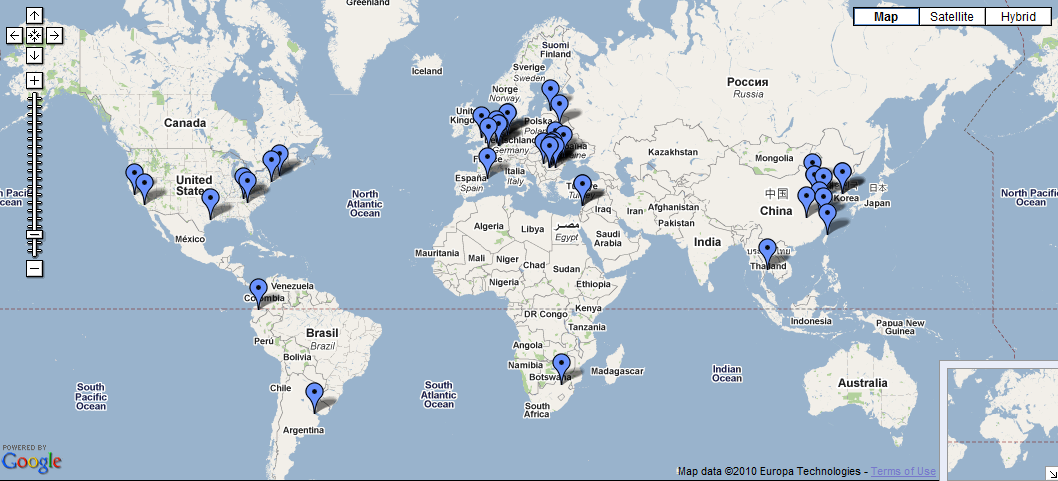
\includegraphics[width=\textwidth]{bin/ssh-geoip.png}\end{center}
    \caption{Map of origins of successful SSH logins}
    \label{pic:ssh-geoip}
\end{figure}
These addresses can then be used with a GeoIP database to look up the location which the network of the address is assigned to.
That has been done in \autoref{pic:ssh-geoip} using a GeoIP tool with a local GeoIP database.
The GeoIP data has to be taken with a grain of salt though.
Firstly, the database might not be correct, simply because network address allocation might have been changed over the recent months\footnote{One could check whether coresponding RIPE entries have been updated though}.
Secondly, the attacker may very well have used a proxy to tunnel the connection through.

There is nothing we can do about proxied connections but we can try to revert the GeoIP database to the state of when the honeypot traffic was captured: January 2009.
Knowing people in the industry, we were able to get network allocation information for the first quarter of 2009.
This information was used to ``update'' the local GeoIP database to make it reflect the earlier network topology.

\begin{figure}
    \begin{center}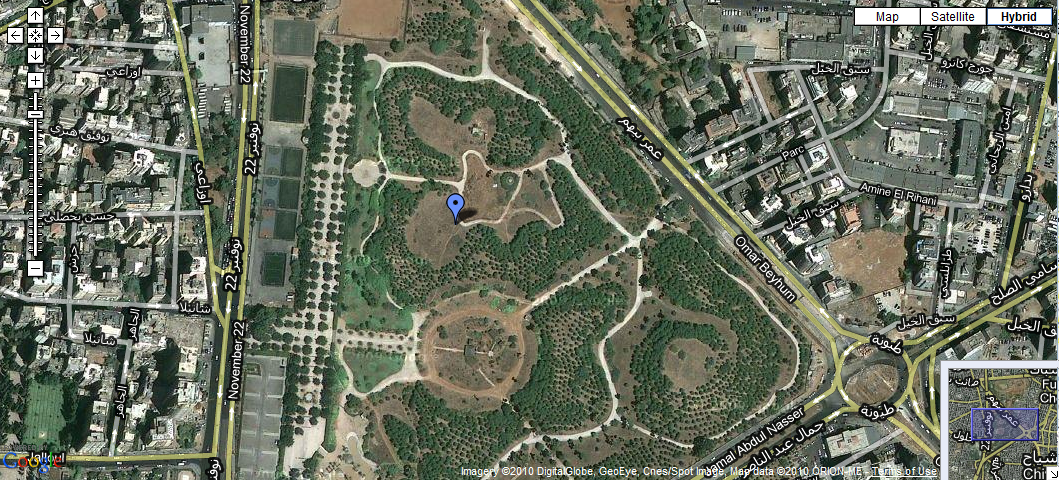
\includegraphics[width=\textwidth]{bin/ssh-geoip-iran.png}\end{center}
    \caption{Lonely hacker sitting in a park in Iran}
    \label{pic:iranian-hacker}
\end{figure}


As already mentioned, SSH is the protocol of choice for logging in to the honeypot so it comes as no surprise that it shows up as the most used protocol in the protocol breakdown.
However, SSH traffic was caused by the attackers trying to brute force SSH accounts on other machines.
This can be seen either in a Snort log mentioned below or in the serial I/O database:

\begin{verbatim}
2009-01-15 00:15:51|ssh-scan
[...]
2009-01-27 17:27:09|#######################################
2009-01-27 17:27:10|###  Just another ssh brute tool  ###
2009-01-27 17:27:10|###     sunny rain & sunny days     ###
2009-01-27 17:27:10|###        here comes the sun      ###
2009-01-27 17:27:10|./a: line 12:  1547 Segmentation fault  ./pscan2 \$1
\end{verbatim}
So a tool searching for username/password combinations was eventually run.
However, the tools were obviously either written poorly or the attackers did not know how to handle them.
In the serial I/O output given above, the most likely self-written tool crashed right away.
This might indicate the level of experience of the attackers.






Another interesting fact we found was that the attacker obtained information about the installed CPU.
While that is a pretty normal thing to do, we found the results doubtful:
\begin{verbatim}
2009-01-15 00:04:03|model name
2009-01-15 00:04:04|: Pentium II (Klamath)
2009-01-15 00:04:04|stepping
2009-01-15 00:04:04|: 3
2009-01-15 00:04:04|cpu MHz
2009-01-15 00:04:05|: 2788.439
2009-01-15 00:04:05|cache size
2009-01-15 00:04:05|: 2048 KB
\end{verbatim}
A Pentium II Klamath, released more than ten years ago in 1997, never had almost 3GHz nor 2MB Cache\footnote{cmp. \url{http://en.wikipedia.org/wiki/Pentium_II\#Klamath}}.
So the CPU string must have been overwritten by the Honeypot administrator.


To get an idea of how compromised the honeypot was, we identified to number of user accounts that were broken into.
The list of user account was obtained \texttt{grep}ping through the serial I/O database for strings that match a regular bash pattern, namely ``username@hostname''.
The compromised users are
\begin{inparaitem}
    \item ales
    \item ftpuser
    \item gabriela
    \item test
    \item virgin
    \item sales
    \item service
    \item test
    \item virgin
    \item visa
    \item vpn
    \item webmaster
\end{inparaitem}.
Also the \emph{root} account was pwned by the attacker.
She used an account, which she broke into (gabriela), and elevated her privileges using \texttt{sudo} (on 2009-01-15 10:07:52).

It is also noteworthy, that the first malicious activity took place on  Jan 14 17:46:06, just 20 minutes after the honeypot was put online.
The accout ``sales'' was broken into via SSH from  219.146.252.203, which is most likely located in Qingdao, China.





\section{Slammer Worm} \label{sec:slammer}

During a group meeting, we reasoned that a NOP\footnote{\url{http://en.wikipedia.org/wiki/NOP}} slide would be present in a piece of shell attack code and so a search through the network pcap file for a sequence of NOPs was performed.
A tool called \texttt{ngrep}\footnote{\url{http://ngrep.sourceforge.net/}} was used to search for this byte sequence.

\begin{verbatim}
ngrep -q -t -I jubrowska-capture_1.cap -X '0x9090909090'
\end{verbatim}

This returned a number of matches like the following.
\begin{verbatim}
U 2009/01/25 15:19:56.970303 194.225.233.248:2347 -> 212.110.251.3:1434
  .......................................................................
  .......................B.........p.B.p.B......h...B.....1...P..5..P..Qh
  dllhel32hkernQhounthickChGetTf.llQh32.dhws2_f.etQhsockf.toQhsend..B.E.P
  P.E.P.E.P..P...B....=U..Qt.....B....1.QQP.........Q.E.P.E.P..j.j.j..P.E
  .P.E.P.......<a...E...@...........).....E.j..E.P1.Qf..x.Q.E.P.E.P....
\end{verbatim}
A google search with a portion of the printable characters indicated that this was probably the SQL Slammer worm.
Now knowing our target, we furthur refined our search using the slammer signature \texttt{0401010101010101} obtained online from Cisco.\footnote{\url{http://www.cisco.com/global/EMEA/sitewide_assets/pdfs/tdm/threat/sqlsw_wp.pdf}}

\begin{verbatim}
ngrep -q -t -I jubrowska-capture_1.cap -X '0401010101010101' | less
\end{verbatim}

We found a total of 104 matches for our match expression in the 700 megabyte pcap file.

Doing that sort of matching manually is a tedious and error prone task.
So we tried to use an Intrusion Detection System (IDS) to do an automated detection of malicious traffic.
We ran Snort against the pcap file and interestingly enough it did not show the Slammer worm propagation attempts on our first try.
We had to modify Snorts configuration to include the ``virus'' rules (which did not work out of the box) before Snort finally detected the malicious payloads. We generated the the snort log file as follows:

\begin{verbatim}
snort -r /home/anthony/uni/forensics/jubrowska-capture_1.cap \
    -c /root/snort/snort.bleeding.conf -A console > console-alerts
\end{verbatim}

During the analysis of the Snort logs which contained 832127 log entries, we noted that only 22976 entries related to a mixture of port scans, and worms.
While the remaining 809151 entries related to SSH in some way.
An example of some of the log entries in the snort scan can be seen below.

\begin{verbatim}
01/23-11:02:31.001196  [**] [1:2500264] BLEEDING-EDGE COMPROMISED
    Known Compromised or Hostile Host Traffic (265) [**]
    [Priority: 0] {TCP} 83.7.245.204:22 -> 212.110.251.3:37761
01/23-11:02:31.026947  [**] [1:2001219] BLEEDING-EDGE Potential SSH Scan
    [**] [Classification: Attempted Information Leak] [Priority: 2]
    {TCP} 212.110.251.3:57172 -> 83.7.246.104:22
\end{verbatim}

The first log entry highlights that some known compromised traffic was seen in the pcap file.
The second entry highlights a potential SSH scan.
%\FIXME{Maybe map the target IP addresses No time to do this.}




\section{DAVIX Scripts}  \label{sec:davix}
At various stages during the analysis, we made use of the scripts included in the DAVIX image.
These were useful as a summary of the events in the pcap files, though on their own were of limited use.
There were, however, some interesting features that they helped us to reveal.

Many of the scripts proved useless in this particular instance.
For example, the script to display HTTP traffic gave no important information as there was barely any HTTP traffic at any stage of the capture.

Conversely, the script (\texttt{006\_activity\_connections\_tcp\_ports.sh}) to map out TCP traffic was far more useful.
The script extracts information on TCP between IPs in the capture and renders the result as a map in Afterglow.
We used this tool to examine each section of the capture.
For the most part the results seemed relatively normal, however we did find an unusual surge of traffic in the ninth section.

\begin{figure}
    \begin{center}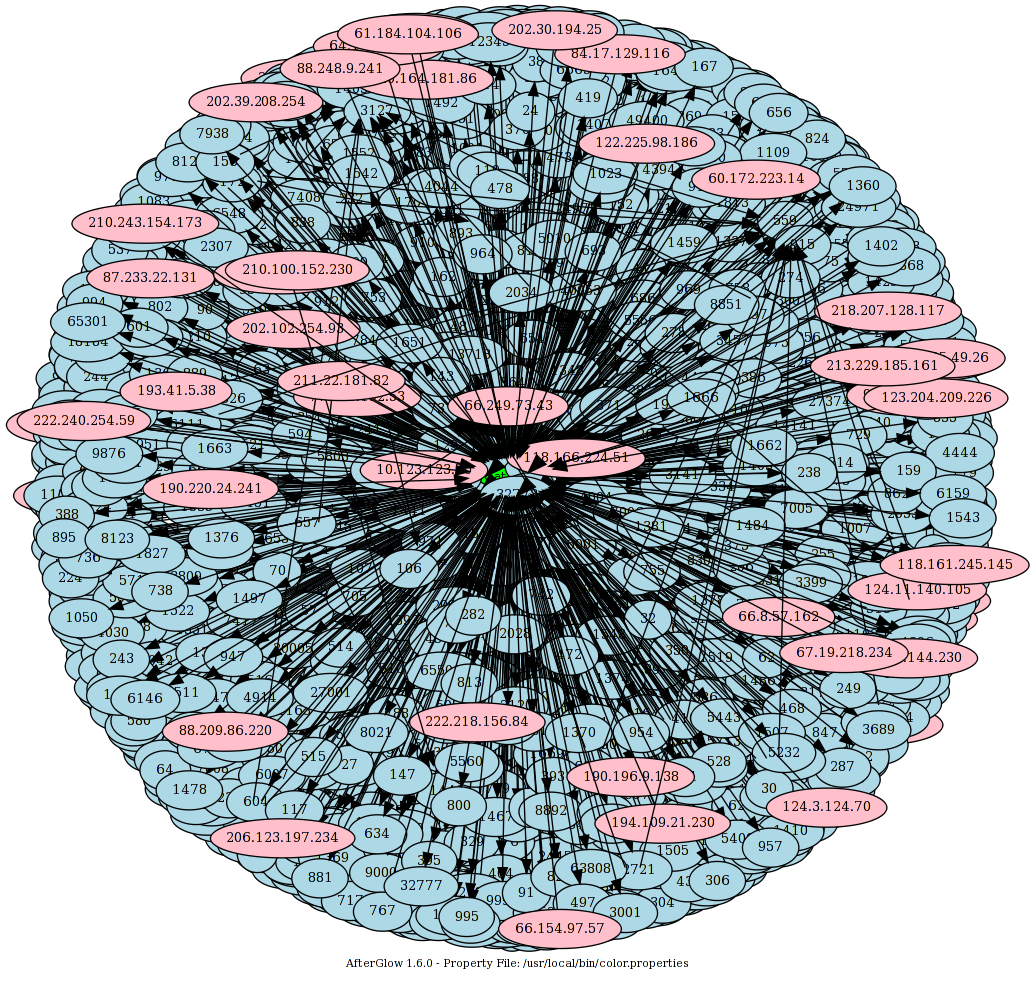
\includegraphics[width=\textwidth]{bin/09_messy.png}\end{center}
    \caption{Surge of TCP Traffic}
    \label{pic:messy_chart}
\end{figure}

Using the script \texttt{012\_activity\_tcpdstport\_r.sh} we were able to plot all the destinations of the TCP traffic to a chart in R.
At four points in this chart we can see vertical lines, indicating a surge in TCP traffic across many ports.
We can see that there is far more activity around the lower ports and it eases off towards the higher ones.
The nature of these lines, combined with the observations made earlier, would indicate that a port scan is taking place.

\begin{figure}
    \begin{center}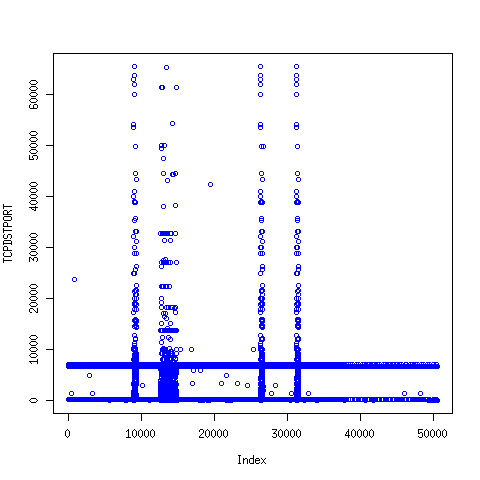
\includegraphics[width=\textwidth]{bin/09_tcp_r.png}\end{center}
    \caption{TCP Port Activity, a close up of \autoref{pic:dest-ports-over-time}}
    \label{pic:tcp_r}
\end{figure}

There are also two heavy blue lines across many of the plots generated by this script.
One is just above 0, so it would make sense to assume that this is port 80 and what we are seeing is standard network traffic.
The second is a bit below 10000.
Given that we know there was a lot of IRC traffic during the capture, this is likely port 6667 as this is usually used for IRC.

Another tool which was somewhat useful was the script for mapping IP addresses to their appropriate MAC addresses.
However, some modification was needed to maximise its usefulness.
One problem, for example, was that so many IPs were used during the capture that Afterglow would run out of memory and crash when trying to render some of the more complex parts of the capture file.
We managed to fix this by applying a subnet filter to any IP addresses collected, therefore cutting the amount of nodes needed to be rendered to just a fraction of what it was. The filter was implemented by replacing the line:

\verb#cat d_ip_mac.csv | sort | uniq > d_ip_mac_distinct.csv#

with:

\begin{verbatim}
cat d_ip_mac.csv | sed -e s'/212\.110\.251\.3/Honeypot/g'|
    sed -e s'/208\.67\.222\.222/Gateway/g' |
    sed -e s'/\.[0-9]*\.[0-9]*\,/\.0\.0\,/g'|
    sort | uniq > d_ip_mac_distinct.csv
\end{verbatim}

This also renamed the IPs \texttt{212.110.251.3} to ``Honeypot'' and \texttt{208.67.222.222} to ``Gateway''.
This served two purposes; Firstly, it meant that the Gateway and Honeypot were easy to find amongst all the numbers in the diagram.
Secondly, it prevented these two important IPs from being removed by the filter.
We also edited the \texttt{color.properties} file associated with Afterglow to give each important element their own colour.

\begin{figure}
    \begin{center}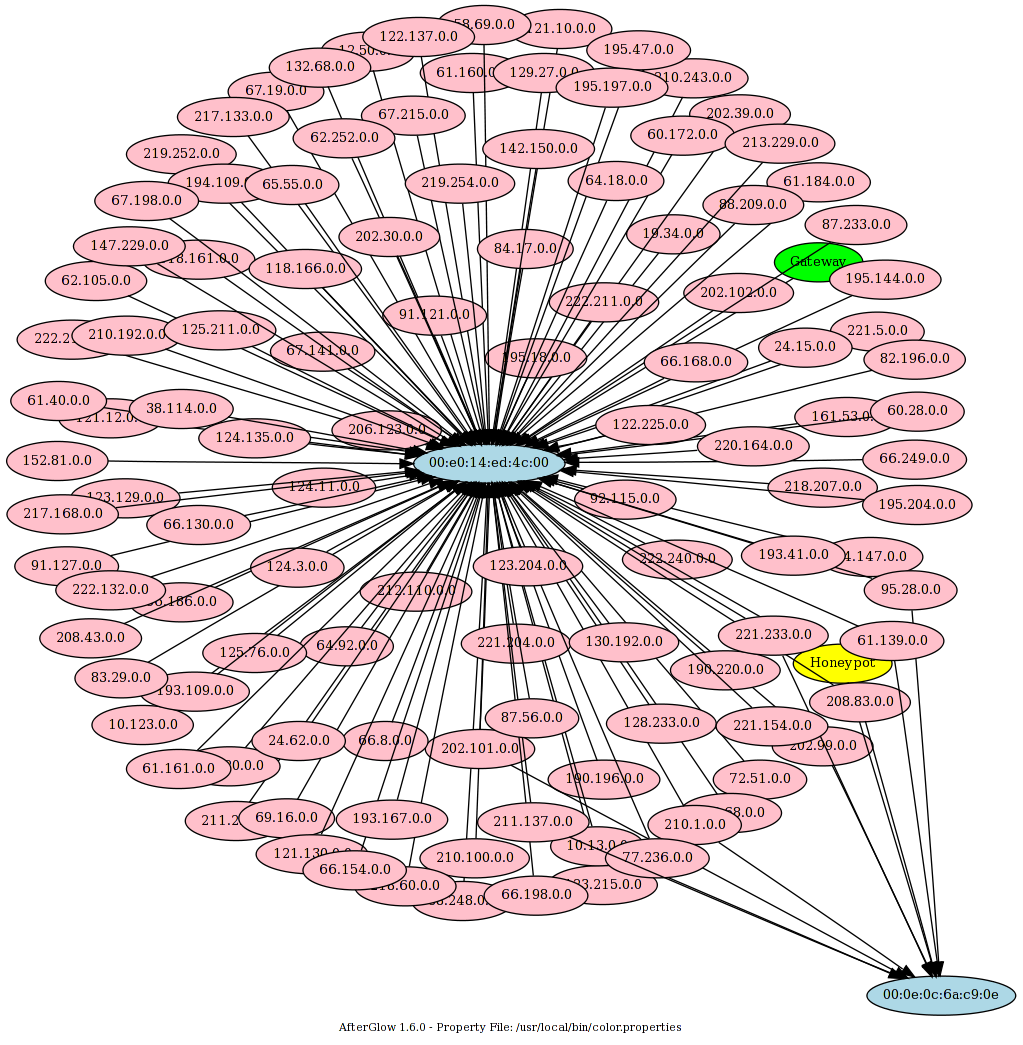
\includegraphics[width=\textwidth]{bin/colourmap.png}\end{center}
    \caption{IP to MAC mappings}
    \label{pic:colourmap}
\end{figure}






\section{IRC Traffic} \label{sec:irc-traffic}
We did some analysis on the IRC traffic contained in the pcap file using \texttt{ngrep} which outputs everything as standard ASCII text by default.

\begin{verbatim}
ngrep -q -I jubrowska-capture_1.cap PRIVMSG | less
\end{verbatim}

Below you can see a small portion of the IRC traffic.
Getting Google Translate\footnote{\url{http://translate.google.com/}} to translate this text revealed it to be Romanian or some language close to this.
Another interesting observation is that the attackers were talking in an IRC chatroom (Channel) \texttt{\#malldova}.
Although we could follow the conversation being made via IRC\footnote{We consider it an interesting question legal and moral whether this conversations have to be treated as private communication} we could not really make sense out of it, because we do not speak Romanian or Moldovian.
We were, however, able to extract some parts which talked about a city in Moldovia.
By further observing the nicknames the attackers chose and the way they talk, we could probably identify the actual persons that launched the attacks.


\begin{verbatim}
T 208.83.20.130:6667 -> 212.110.251.3:46937 [AP]
  :Alejik!AleG_20@1albaiulia.users.undernet.org PRIVMSG
  #CaNaL+ :eu si eri am intrat si tu pleci si azi tot asa :) nu e bine ..

T 195.47.220.2:6667 -> 212.110.251.3:59407 [AP]
  :D_12!~D12@D12UP.users.undernet.org PRIVMSG #CaNaL+ :_AngeloS_..
\end{verbatim}



As indicated in \autoref{sec:intro}, IRC packets was by far the most dominant type of captured traffic.
Interestingly, the massive number of IRC packets was generated in just a fifth of the overall packet capture as per \autoref{pic:dest-ports-over-time}.
This fact can be explained by looking at the serial I/O database (cmp.\, \autoref{sec:http-traffic} as well as the captured packets.
The attacker downloaded and ran \emph{EnergyMech}, an ``Open source IRC bot written in C. Includes many useful features''\footnote{\url{http://www.energymech.net/}}.
The captured packets show that the IRC bot was constantly trying to reconnect to the UnderNet IRC network.
This also explain the massive number of DNS queries, because the bot resolved the IP addresses for the IRC network before trying to connect to it.
The reconnections were caused by the attackers not being able to properly configuring their software.
The bot tried to log in to the IRC service but the chosen nicknames were taken so that the server denied access.
Reconnection attempts of the bot resulted in it being blocked because the reconnects were tried to quickly.











\section{Conclusion} \label{sec:conclusion}

We spent a lot of time researching and evaluating tools that could visualise the massive amount of data in the jubrowska pcap file.
The potential tools for visualising data were assessed and critiques were given.
Most of the tools did not satisfy us because they were either not properly network aware or could not cope with our big amount of data.

Also, a general overview over the given network traffic capture, as well as the serial I/O database was given.
We identified IRC, DNS and SSH as the most spoken protocols.
SSH did not come as a surprise because it is the protocol of choice to connect to the honeypot as well as other target machines.
The DNS and IRC traffic were identified to be related in a way: The attackers were not able to configure their IRC bots properly which resulted in constant reconnects to different IRC servers.


Using the tools included in the DAVIX image we were able to visualise the network at various times during the trace. Peaks in TCP traffic at certain times and unusually heavy IRC activity led us to investigate further and uncover the nature of the attack.

Traffic relating to the Slammer worm was identified by first searching fot NOP slides and then later for the worm signature string.

Other types of traffic, including HTTP, SSH and IRC, was analysed and each investigation yielded information that is not only able to identify the attack but also to potentially pinpoint the attackers.
We thus found out that at least some of the attackers are most likely located in Moldova.

Surely, we could further investigate simply because the amount of data is huge.
Further analysis could produce more pictures that have a time dimension or create an animation of the changes of some visualised information.

%\appendix
%\pagebreak
% \nocite{*}
% \bibliographystyle{geralpha}
% \bibliographystyle{apasoft}
% \bibliographystyle{cell}
%\bibliographystyle{apalike}
% Well, you the forensics.bib. Either just create an en empty one or clone the Mercurial repository:
% hg clone https://hg.cryptobitch.de/ss10-ca643-forensic
% and work insides the Labs directory.
% If you have changes, first pull latest changes to make sure your changes apply cleanly to the most recent version:
% hg pull && hg merge
% If there are conflicts, you might want to have kdiff3 or meld installed.
% After having merged changes (check with hg heads), do a
% hg bundle /tmp/mychanges.bundle
% and send me the bundle file.
% To create changes, simple edit the file in question, save, and do a "hg ci".
%\bibliography{forensics}

\section*{License}
This work is licensed to the public under the Creative Commons Attribution-Non-Commercial-Share Alike 3.0 Germany License.
\begin{center}
\includegraphics{bin/by-nc-sa-eu.png}\end{center}


\end{document}

